\documentclass[preprint,12pt]{elsarticle}
\usepackage[margin=1in]{geometry} 
\usepackage{graphicx}
\usepackage{amsmath,amsthm,amssymb,amsfonts, fancyhdr, color, comment, graphicx, environ}
%\usepackage[style=ieee, citestyle=numeric-comp, backend=biber]{biblatex}
%\addbibresource{library.bib}
\usepackage{xcolor}
\usepackage{mdframed}
\usepackage{svg}
\usepackage{verbatim}
\usepackage[shortlabels]{enumitem}
\usepackage{indentfirst}
\usepackage{hyperref}
\usepackage[utf8]{inputenc}
\usepackage{amsmath}
\usepackage{float}
\usepackage{subfig}
\usepackage[T1]{fontenc}
\renewcommand{\footrulewidth}{0.8pt}
%\usepackage{subcaption}
\hypersetup{
    colorlinks=true,
    linkcolor=blue,
    filecolor=magenta,      
    urlcolor=blue,
}
\providecommand{\keywords}[1]
{
  \small	
  \textbf{\textit{Keywords---}} #1
}
\author{}
\date{}

\journal{Engineering Fracture Mechanics}
\begin{document} 
\begin{frontmatter}

	\begin{abstract}
		\input{abstract}
		
	\end{abstract}
	\begin{keyword}
		Interpretable Machine learning \sep GPSR \sep semi-elliptical surface crack \sep mechanics based training	
	\end{keyword}
	
\end{frontmatter}

\section{Introduction}
Finite element analysis (FEA) is highly effective at calculating stress intensity factors (SIFs) for cracks in arbitrary geometries. However, despite its accuracy, FEA has notable limitations. One significant drawback is its demanding computational requirements, as well as the need for a skilled analyst to achieve reliable results. These factors can lead to substantial time and resource investments, especially when numerous calculations are required, such as those for fatigue and uncertainty assessment. To address these challenges, many engineers in industry often rely on handbook solutions. These solutions offer a practical way to estimate SIFs for common, simplified crack scenarios, and when applied correctly, they can yield very accurate results. Additionally, they entail significantly reduced computational costs compared to FEA.


The Raju Newman equations are widely used set of handbook equations that provide predictions for SIFs under various crack shapes and loading conditions \cite{RNeqnsbook}. These handbook solutions are user-friendly, given their straightforward polynomial forms. However, their ease of use sometimes leads to their application in situations that do not align with the assumptions and limitations of the original idealized model, resulting in inaccurate predictions. This research specifically focuses on the case of a semi-elliptical surface crack in a finite plate subjected to mode I tension. Raju and Newman have an equation designed for this particular crack scenario. Since the introduction of the Raju Newman equations for a semi-elliptical surface cracks alternative models have been proposed that allow for more complex loading conditions such as the models created by \cite{Wang1995, Pommier1999}. The model created by Wang and Lambert allows for linear stress functions \cite{Wang1995}. Pommier, et al. created a model that could predict SIFs under polynomial stress fields \cite{Pommier1999}.

 To prevent the improper use of SIF equations, it is crucial to build a more extensive database of SIF solutions. Machine learning (ML) can play a pivotal role in automating the creation of these SIF solutions. ML enables the development of models for more complex crack scenarios, going beyond the scope of current handbook solutions, which primarily cover idealized cases. Notably, ML has been successfully employed to produce highly accurate SIF solutions, as documented in studies such as in \cite{Zhang2023, Sobotka2022, Keprate2017, Xu2022, Seghier2020}. The advantage of ML over other techniques, like those found in \cite{RNeqnsbook, Pommier1999, Wang1995}, is its ability to be trained relatively quickly, resulting in very accurate models. This, in turn, facilitates the creation of more surrogate models. However, it's worth noting that many commonly used ML algorithms generate "black-box" models, which lack interpretability. In engineering, interpretability is crucial because engineers need to trust and explain their designs, which black-box models do not readily allow. This is why handbook solutions, such as those in \cite{RNeqnsbook}, continue to be used since they inherently offer interpretability.

This paper specifically studies the case of a semi-elliptical surface crack in a finite plate subjected to mode I tension, a common crack found in pressure vessels. An existing handbook solution by \cite{RNeqnsbook} covers this case. However, more accurate models have been developed using machine learning (ML) techniques, as demonstrated by \cite{Keprate2017, Xu2022, Seghier2020}. These ML models, utilizing methods like Gaussian processes regression and neural networks, offer higher accuracy but produce less interpretable "black-box" models. Notably, the ML models mentioned could predict SIFs at only a single point along the crack front, whereas the Raju-Newman equations can estimate SIFs across the entire crack length.

While ML models provide improved predictive capabilities, their lack of interpretability can be a drawback in certain contexts, especially when it comes to explaining and trusting the predicted SIF. The interpretability of the Raju and Newman equations gives engineers a clear understanding of how SIFs are derived, aiding decision-making and instilling confidence in the results. These equations systematically break down the crack case into subfunctions, each contributing differently to the final SIF predition. For instance, in the case of the semi-elliptical crack, they modify the analytical solution to the embedded ellipse with boundary correction functions, enhancing the inherent explainability of an analytical solution.

This research will utilize an interpretable machine learning code Bingo, developed by researchers at NASA and the University of Utah \cite{Randall2022}. Bingo generates closed-form mathematical expressions to predict SIFs along the entire crack length, offering improved accuracy and simplicity compared to the Raju-Newman equations while preserving interpretability. Thanks to the closed-form nature of Bingo's models, they can be easily integrated into existing Linear Elastic Fracture Mechanics (LEFM) software applications like NASGRO, AFGROW, and SMART|DT \cite{nasgro, afgrow, smartdt}. Closed form solutions can also be inverted to solve for applied stress for use in a constant SIF test.

\subsection{Background}
In linear elastic fracture mechanics (LEFM), the precise solution for the Stress Intensity Factor (SIF) along an elliptical crack in an infinite volume is given by the equation:

\begin{equation} \label{eqn:K_embedded_ellipse}
    K_{ee} = \sigma \frac{\sqrt{\pi a}}{E} \left( \sin^2 \phi + \frac{a^2}{c^2} \cos^2 \phi \right)^{1/4}, \text{where } a \le c, 
\end{equation}

where $a$ represents the length of the minor axis of the ellipse, $c$ represents the length of the major axis, $\sigma$ is the far-field stress, and $E$ is the complete elliptic integral of the second kind. This expression is only valid when $a \leq c$. In the context of a semi-elliptical surface crack, the values of $a$ and $c$ differ from the minor and major axes, instead representing the crack depth and half-crack surface length, respectively, as illustrated in figure \ref{fig:crack_params} \cite{tada1985}. To accommodate cases where $a/c$ will exceed 1, Raju and Newman employed a modified version of equation \ref{eqn:K_embedded_ellipse}. This modification, detailed in equation \ref{eqn:fphi}, allows for the use of all values of $a/c$.
\begin{figure}%
    \centering
    \subfloat[\centering Crack dimensions]{{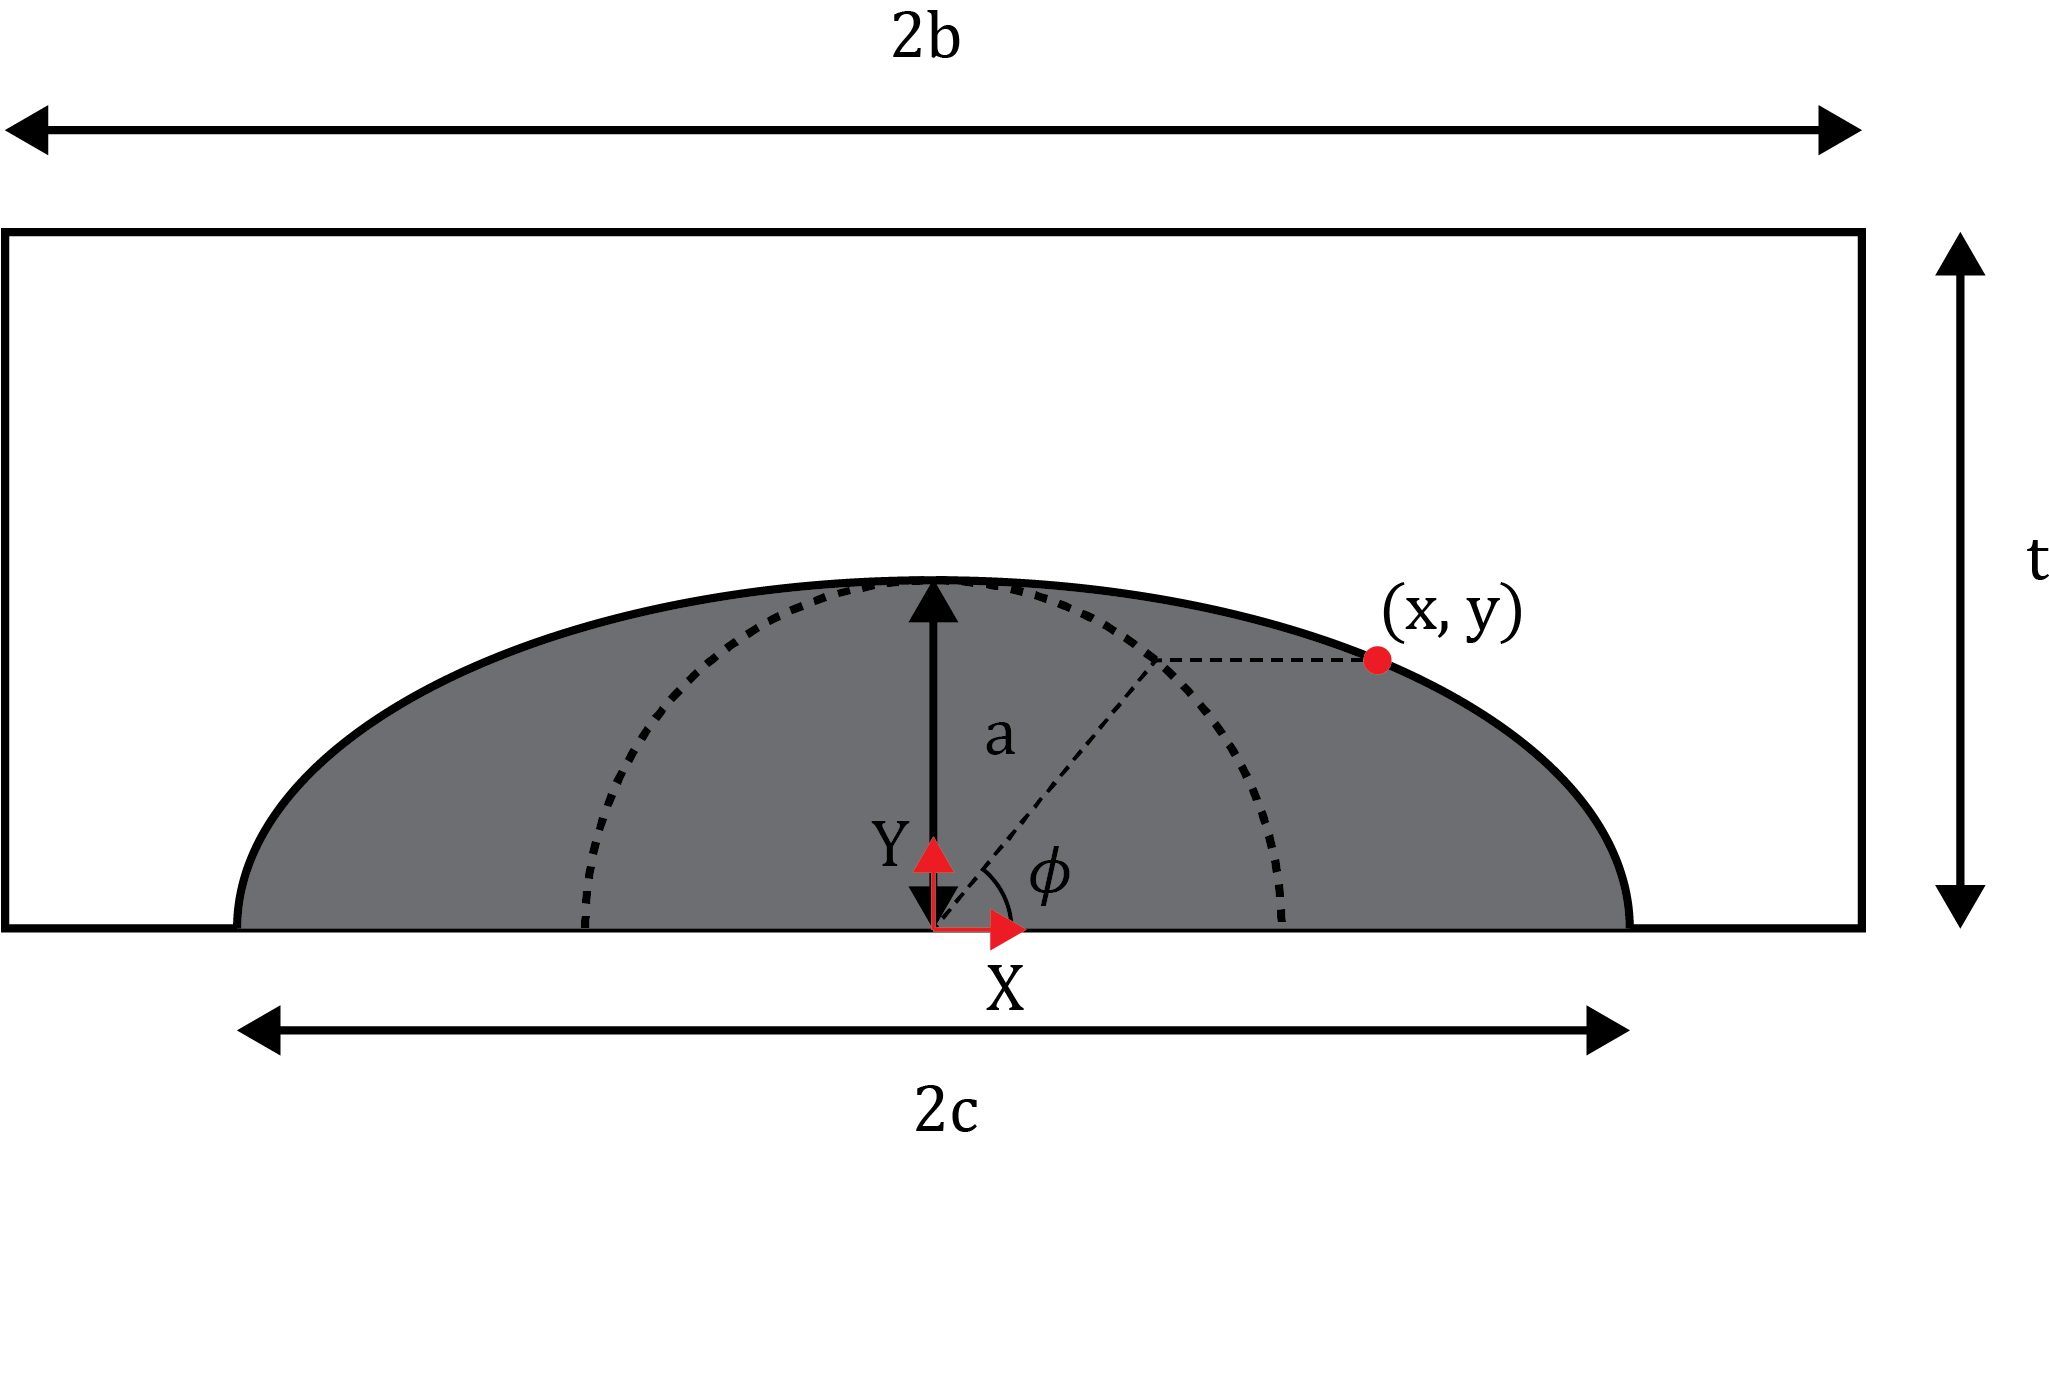
\includegraphics[width=0.5\textwidth]{geometry_figures/params.png} }}%
    \qquad
    \subfloat[\centering Ellipse dimensions]{{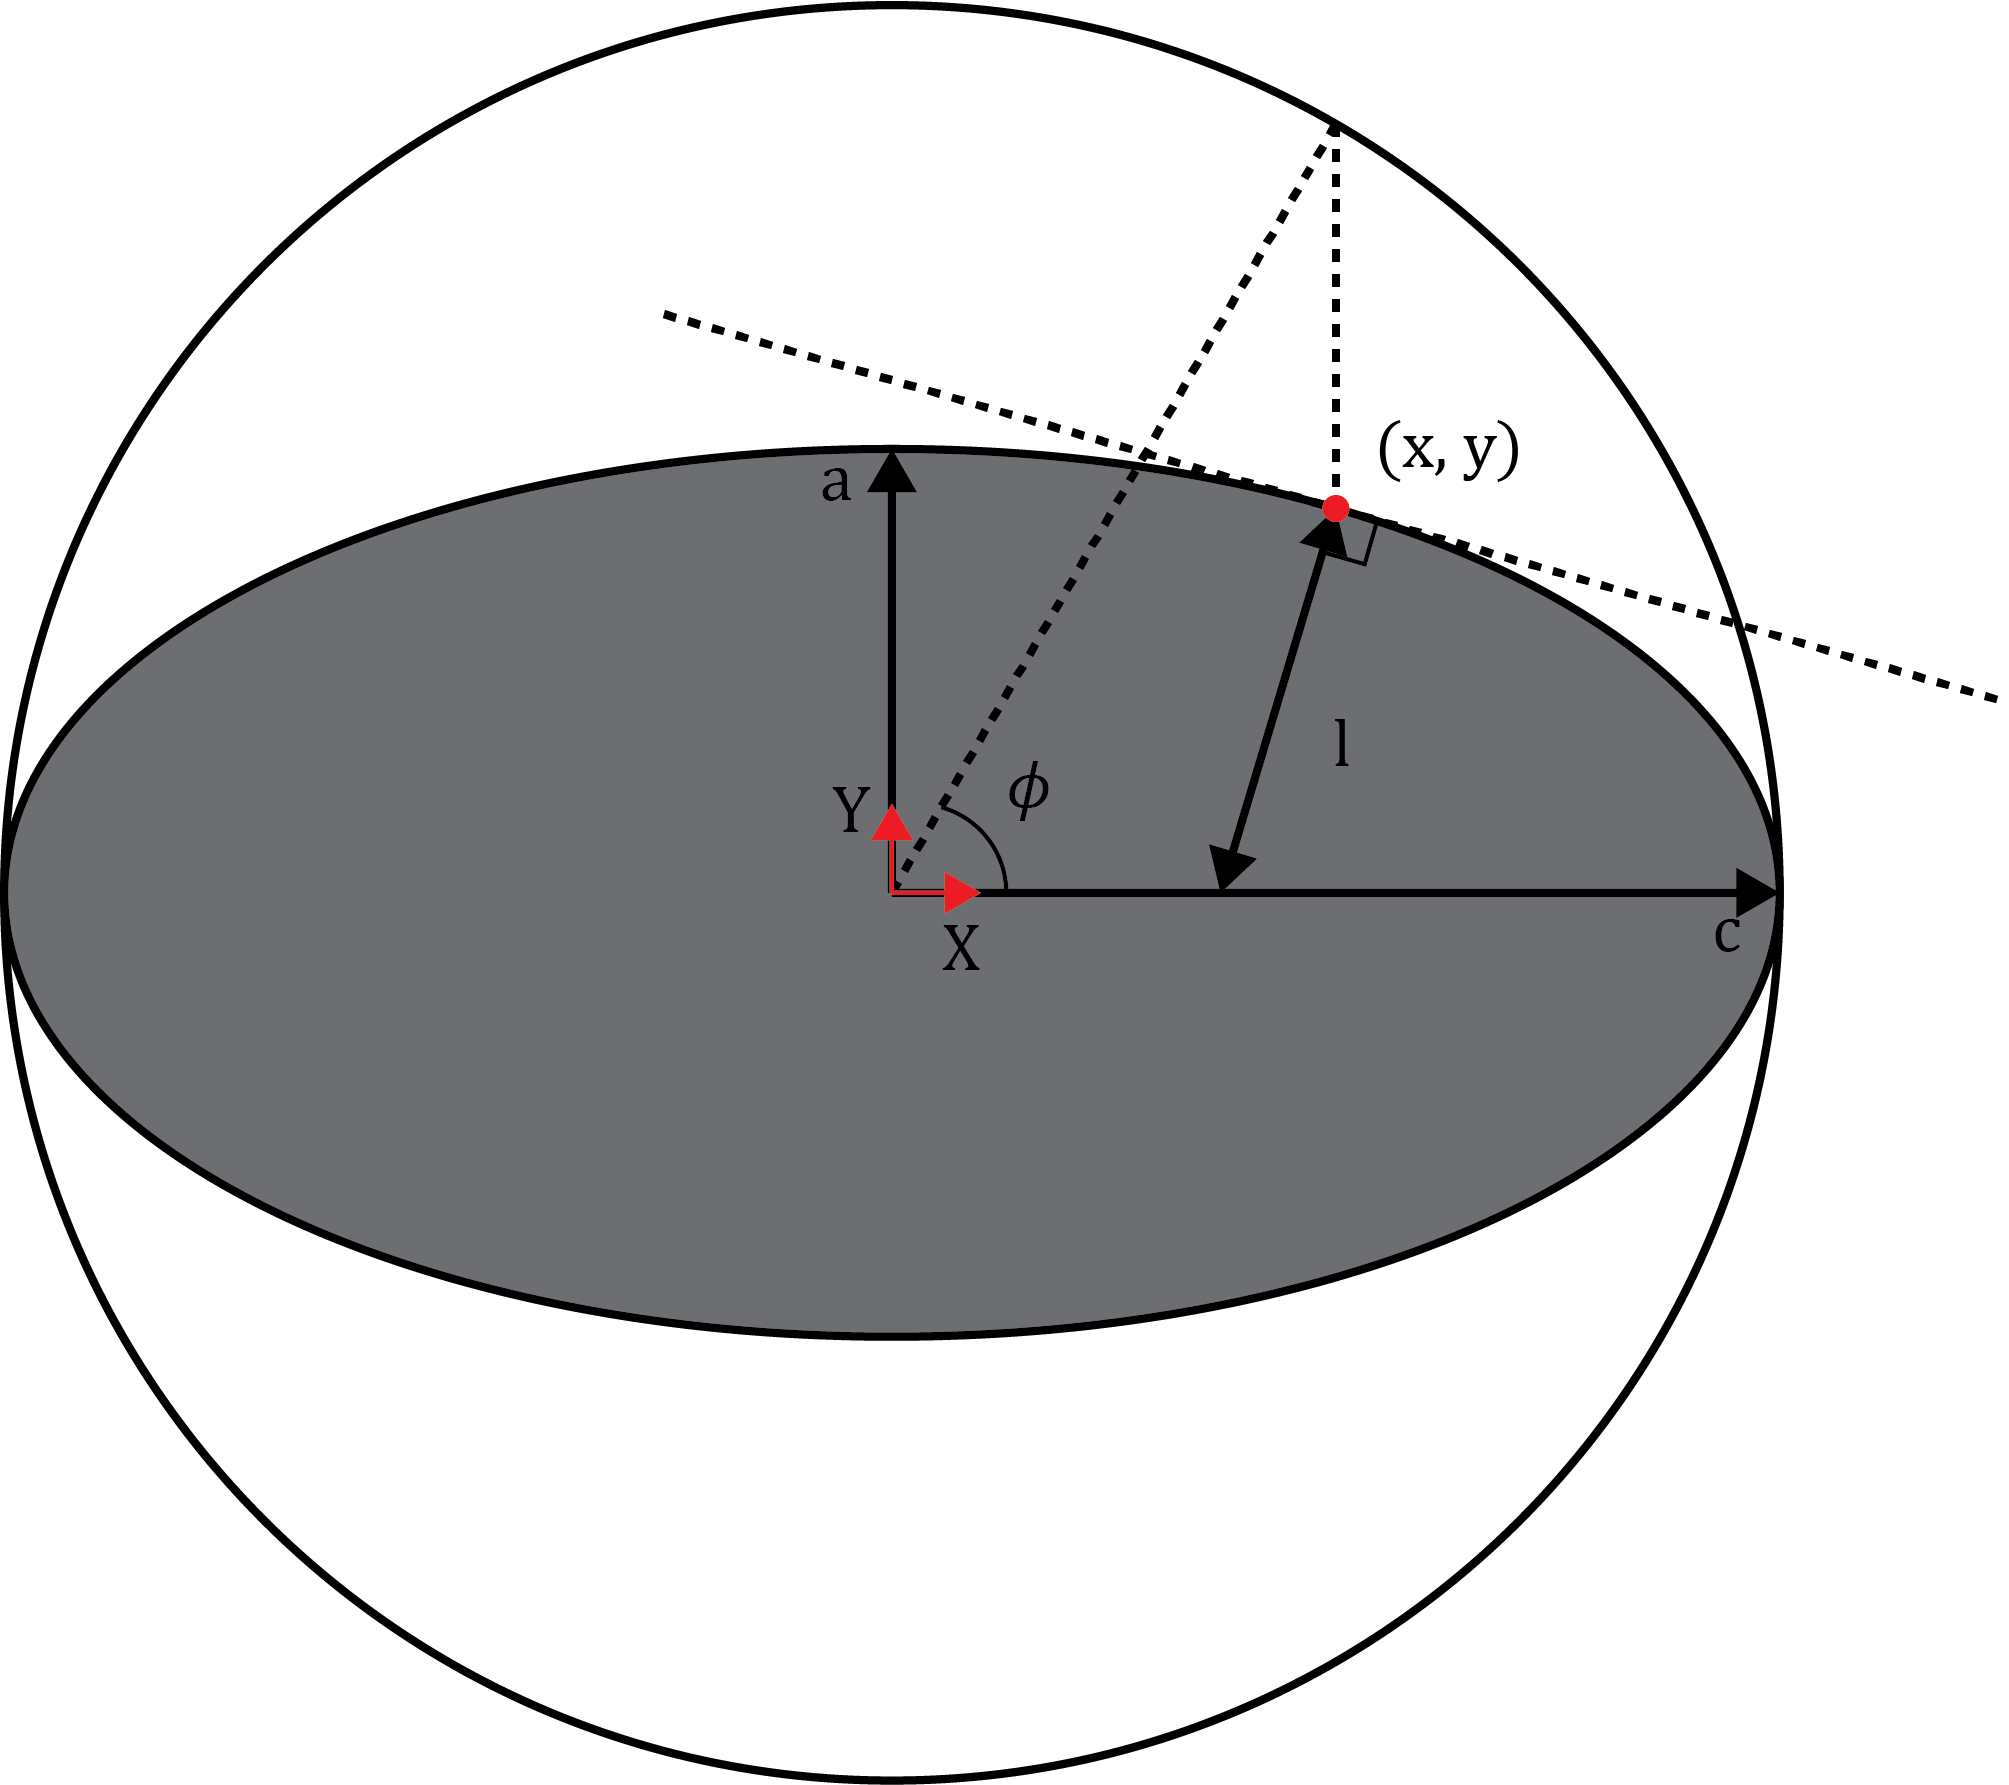
\includegraphics[width=0.5\textwidth]{geometry_figures/Ellipse.png} }}%
    \caption{(a) Crack parameters with $a$ being the crack depth and $2c$ being the surface crack length. (b) $\phi$ is defined by the angle to the inscribed circle projected to the ellipse. $l$ is defined as the distance perpendicular to the tangent line from the point of interest to the nearest axis.}%
    \label{fig:crack_params}%
\end{figure}
\begin{equation} \label{eqn:fphi}
f_{\phi} = \begin{cases}
      \left[\left(\frac{a}{c}\right)^2 \cos^2\phi + \sin^2\phi\right]^{1/4} & \text{if } \frac{a}{c} \le 1 \\
      \\
      \left[\cos^2\phi + \left(\frac{c}{a}\right)^2\sin^2\phi\right]^{1/4} & \text{if } \frac{a}{c} > 1,
    \end{cases}
\end{equation}
 which is piece-wise, resulting in equation \ref{eqn:K_embedded_ellipse_fphi}

\begin{equation} \label{eqn:K_embedded_ellipse_fphi}
    K_{ee} = \sigma \frac{\sqrt{\pi a}}{E} f_{\phi}.
\end{equation}

Equation \ref{eqn:K_embedded_ellipse_fphi} is identical to equation \ref{eqn:K_embedded_ellipse} when $a/c \le 1$. Using equation \ref{eqn:K_embedded_ellipse_fphi} and multiplying by the correction factors $f_w$, $M$, and $g$ Raju and Newman found equation \ref{eqn:RN_K}
 \begin{equation} \label{eqn:RN_K}
     K = \frac{\sqrt{\pi a}}{E} f_{\phi} f_w M g,
 \end{equation} 

which is able to predict SIFs along the length of semi-elliptical surface crack in a finite plate.

The finite width correction factor $f_w$, defined in equation \ref{eqn:RN_fw}
\begin{equation} \label{eqn:RN_fw}
    f_w = \sqrt{\sec\left(\frac{\pi c}{2b}\sqrt{\frac{a}{t}}\right)},
\end{equation}
 is a 3D extension for the equation developed in \cite{brown1966}. The finite width correction factor accounts for the finite width and thickness of the plate when $a/c = 1$ and $\phi = \pi/2$. The thickness of the plate is denoted as $t$ and the half-width of the plate is denoted as $b$ \ref{fig:crack_params}. The function $M$ accounts for changes is SIF due to the aspect ratio of the crack at the point along the crack where $\phi = \pi/2$ and is given by \ref{eqn:RN_M}
\begin{equation} \label{eqn:RN_M}
    M = M_1 + M_2\left(\frac{a}{t}\right)^2 + M_3\left(\frac{a}{t}\right)^4
\end{equation}
\begin{equation} \label{eqn:RN_M1}
    M_1 = \begin{cases}
    1.13 - 0.09\left(\frac{a}{c}\right) & \text{if } \frac{a}{c} \le 1 \\
    \\
    \sqrt{\frac{c}{a}}\left(1 + 0.04\frac{c}{a}\right) & \text{if } \frac{a}{c} > 1
    \end{cases}
\end{equation}
\begin{equation} \label{eqn:RN_M2}
    M_2 = \begin{cases}
    -0.54 + \frac{0.89}{0.2+\left(\frac{a}{c}\right)} & \text{if } \frac{a}{c} \le 1 \\
    \\
    0.2\left(\frac{c}{a}\right)^4 & \text{if } \frac{a}{c} > 1
    \end{cases}
\end{equation}
\begin{equation} \label{eqn:RN_M3}
    M_3 = \begin{cases}
    0.5 - \frac{1}{0.65+\frac{a}{c}} + 14\left(1-\frac{a}{c}\right)^{24} & \text{if } \frac{a}{c} \le 1 \\
    \\
    -0.11\left(\frac{c}{a}\right)^4 & \text{if } \frac{a}{c} > 1.
    \end{cases}
\end{equation}
The function g corrects for free surface effects and is denoted by equation \ref{eqn:RN_g}
\begin{equation} \label{eqn:RN_g}
    g = \begin{cases}
    1 + \left[0.1 + 0.35\left(\frac{a}{t}\right)^2\right]\left(1 - \sin\phi\right)^2 & \text{if } \frac{a}{c} \le 1 \\
    \\
    1 + \left[0.1 + 0.35\left(\frac{c}{a}\right)\left(\frac{a}{t}\right)^2\right]\left(1 - \sin\phi\right) & \text{if } \frac{a}{c} > 1.
    \end{cases}
\end{equation}
The function $g$ is sinusoidal, having a value of 1 at $\phi = \pi/2$.  By using this methodical approach of breaking down the problem into sub-functions that each account for a different aspect of the crack, allowed Raju and Newman to develop accurate equations that build upon the explainablity from the analytical solution of the embedded ellipse. 

\section{Methods}
\subsection{Computational Fracture Mechanics}

The stress intensity factors used in this research were simulated using finite element analysis (FEA) using FRANC3D and Abaqus software \cite{f3d, Abaqus}. Abaqus served as the primary tool for creating the geometry, initial mesh discretization, application of BCs, and solution. FRANC3D was employed for tasks related to crack insertion and SIF computation. Abaqus' Python interface was used to generate the model geometries.

A local-global sub-modeling approach was employed within FRANC3D which involved dividing the geometry into two components: the global model, which encompassed the boundary conditions, and the local model, containing the region where the crack would be inserted. The local model is used in FRANC3D, where the crack is inserted using a crack front template consisting of rings of hexagonal elements, with an inner ring of quarter-point elements surrounding the crack front, allowing for SIF computations Fig. \ref{fig:f3d_mesh}. After crack insertion the local model was re-meshed, preserving the nodal locations on the cut faces (i.e. local-global boundary) for later coherency with the global model. The complete model, with the inserted crack, was subsequently solved using Abaqus. This process is illustrated in Fig. \ref{fig:f3d_abq_flow}.



\begin{figure}
  \centering
  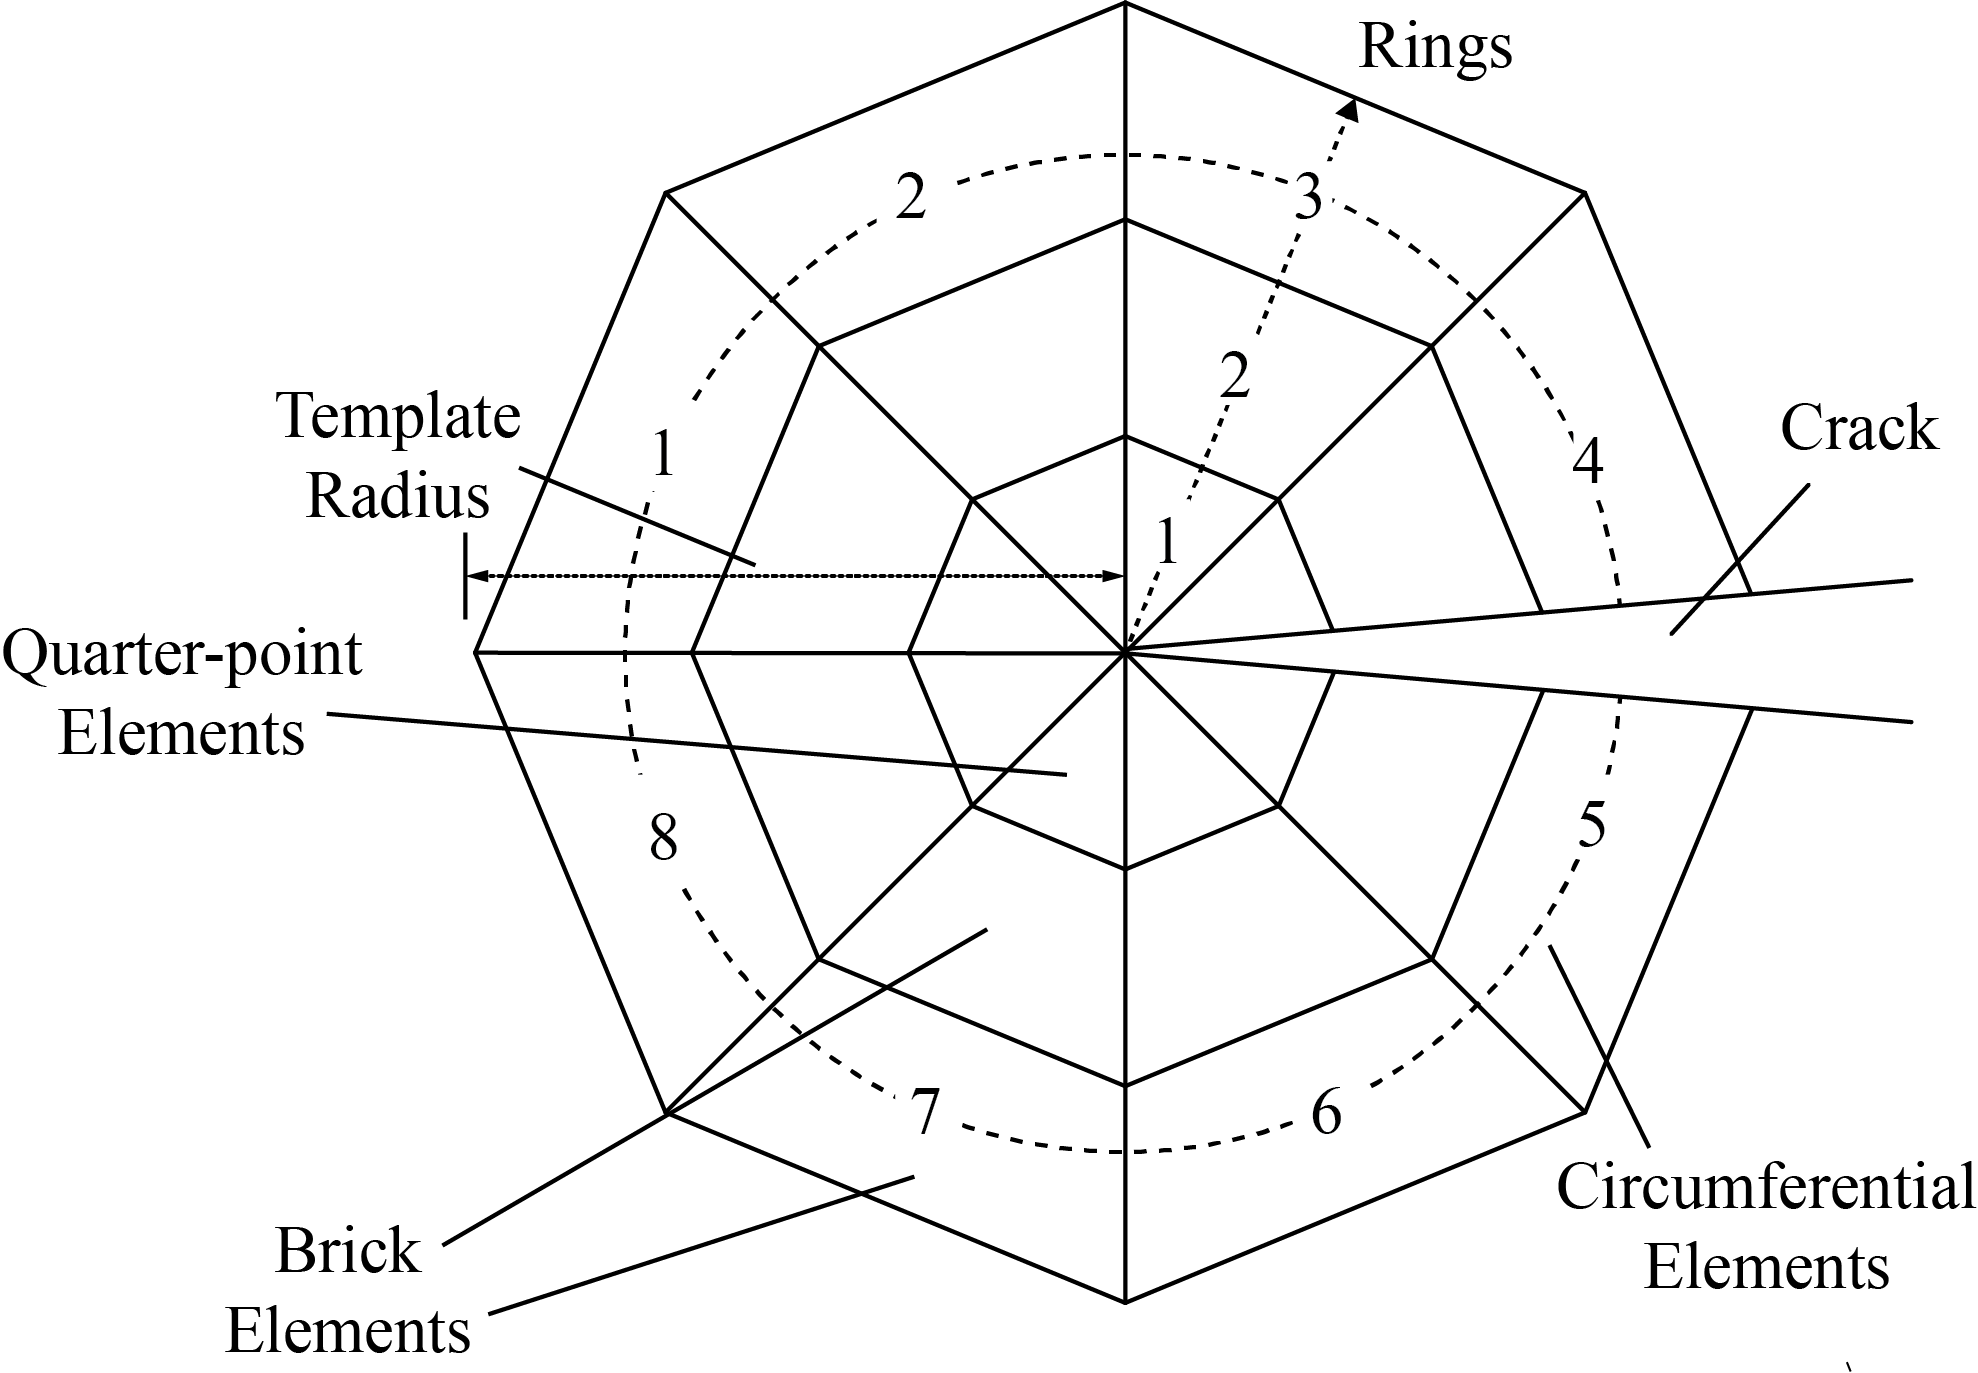
\includegraphics[width=0.8\textwidth]{geometry_figures/f3d_crack.png}
  \label{fig:f3d_mesh}
  \caption{FRANC3D crack mesh containing 8 circumferential elements and 3 rings. The template radius is the radius of an inscribed circle}
\end{figure}

Integral methods are geometrically more accurate than displacement methods, such as displacement correlation, for the computation of SIFs. The J-integral, developed by Rice \cite{Rice1968}, is a commonly used method for SIF calculation. However, it has a limitation, it cannot separate the SIFs into the three cracking modes, except for very simplified crack geometries, as noted by Banks-Sills et al. \cite{Banks-Sills2005}. Banks-Sills et al. developed the M-Integral formulation to overcome this limitation allowing for the calculation of accurarate SIFs for all three cracking modes \cite{Banks-Sills2005}

\begin{comment}

To address this limitation, the M-integral offers a solution by using a combination of two SIFs: one representing the true SIF and the other an arbitrary solution. By employing this approach, it becomes possible to extract each SIF corresponding to the three cracking modes, as explained by \cite{Banks-Sills2005}. The M-integral is defined as follows:

\begin{equation}\label{eqn:M-Integral}
    M^{(1, 2)} = \int_\Gamma \left(W^{(1,2)}n_1 - T^{(1)}_i \frac{\partial u^{(2)}_i}{\partial x_1} - T^{(2)}_i \frac{\partial u^{(1)}_i}{\partial x_1} \right) \, \text{d}s,
\end{equation}

Here, $T_i = \sigma_{ij} n_j$ represents the traction vector, $W = 1/2 \sigma_{ij} \epsilon_{ij}$ stands for the strain energy density, and the superscripts 1 and 2 correspond to the two superposed solutions.
\end{comment}

\subsection{Genetic Programming Based Symbolic Regression}
% look at previous papers to write this Karl, Donovan, Geoff plasticity paper
% https://arxiv.org/abs/2304.01117

Symbolic Regression (SR) is a machine learning technique aimed at discovering closed-form analytical expressions that model training data and known physics \cite{Karl,  Hongsup}. Presently, the most effective optimization approach for SR is genetic programming (GP) \cite{GPSR-comp}. The implementation of genetic programming based symbolic regression (GPSR) employed in this research is an open-source Python package, Bingo \cite{Randall2022}. Bingo enables learning real-valued mathematical expressions represented as acyclic graphs (Agraphs). The equation's complexity is determined by the number of nodes in the Agraph, Fig. \ref{fig:agraph} shows an Agraph for the equation $C_0 X_0 + C_1 X_1$, that has a complexity of 7 corresponding to the 7 nodes in the Agraph. The training begins with an initial assortment of randomly generated equations, varying in complexity. During each generation, equations undergo randomized evolutions, employing a combination of crossover and mutation. Crossover entails exchanging nodes from two Agraphs along with their associated branches and leaves, generating two evolved equations. Mutation introduces random changes to nodes in the Agraph as shown in Fig. \ref{fig:agraph_cross_mut} \cite{Schmidt2007}. After crossover and mutation has occurred the equations are ranked based on a defined fitness function e.g. MAE, RMSE, etc. The most fit equations are then used in the next generation where the cycle continues until a fitness threshold or maximum number of generations has been satisfied. 

\begin{figure}
    \centering
    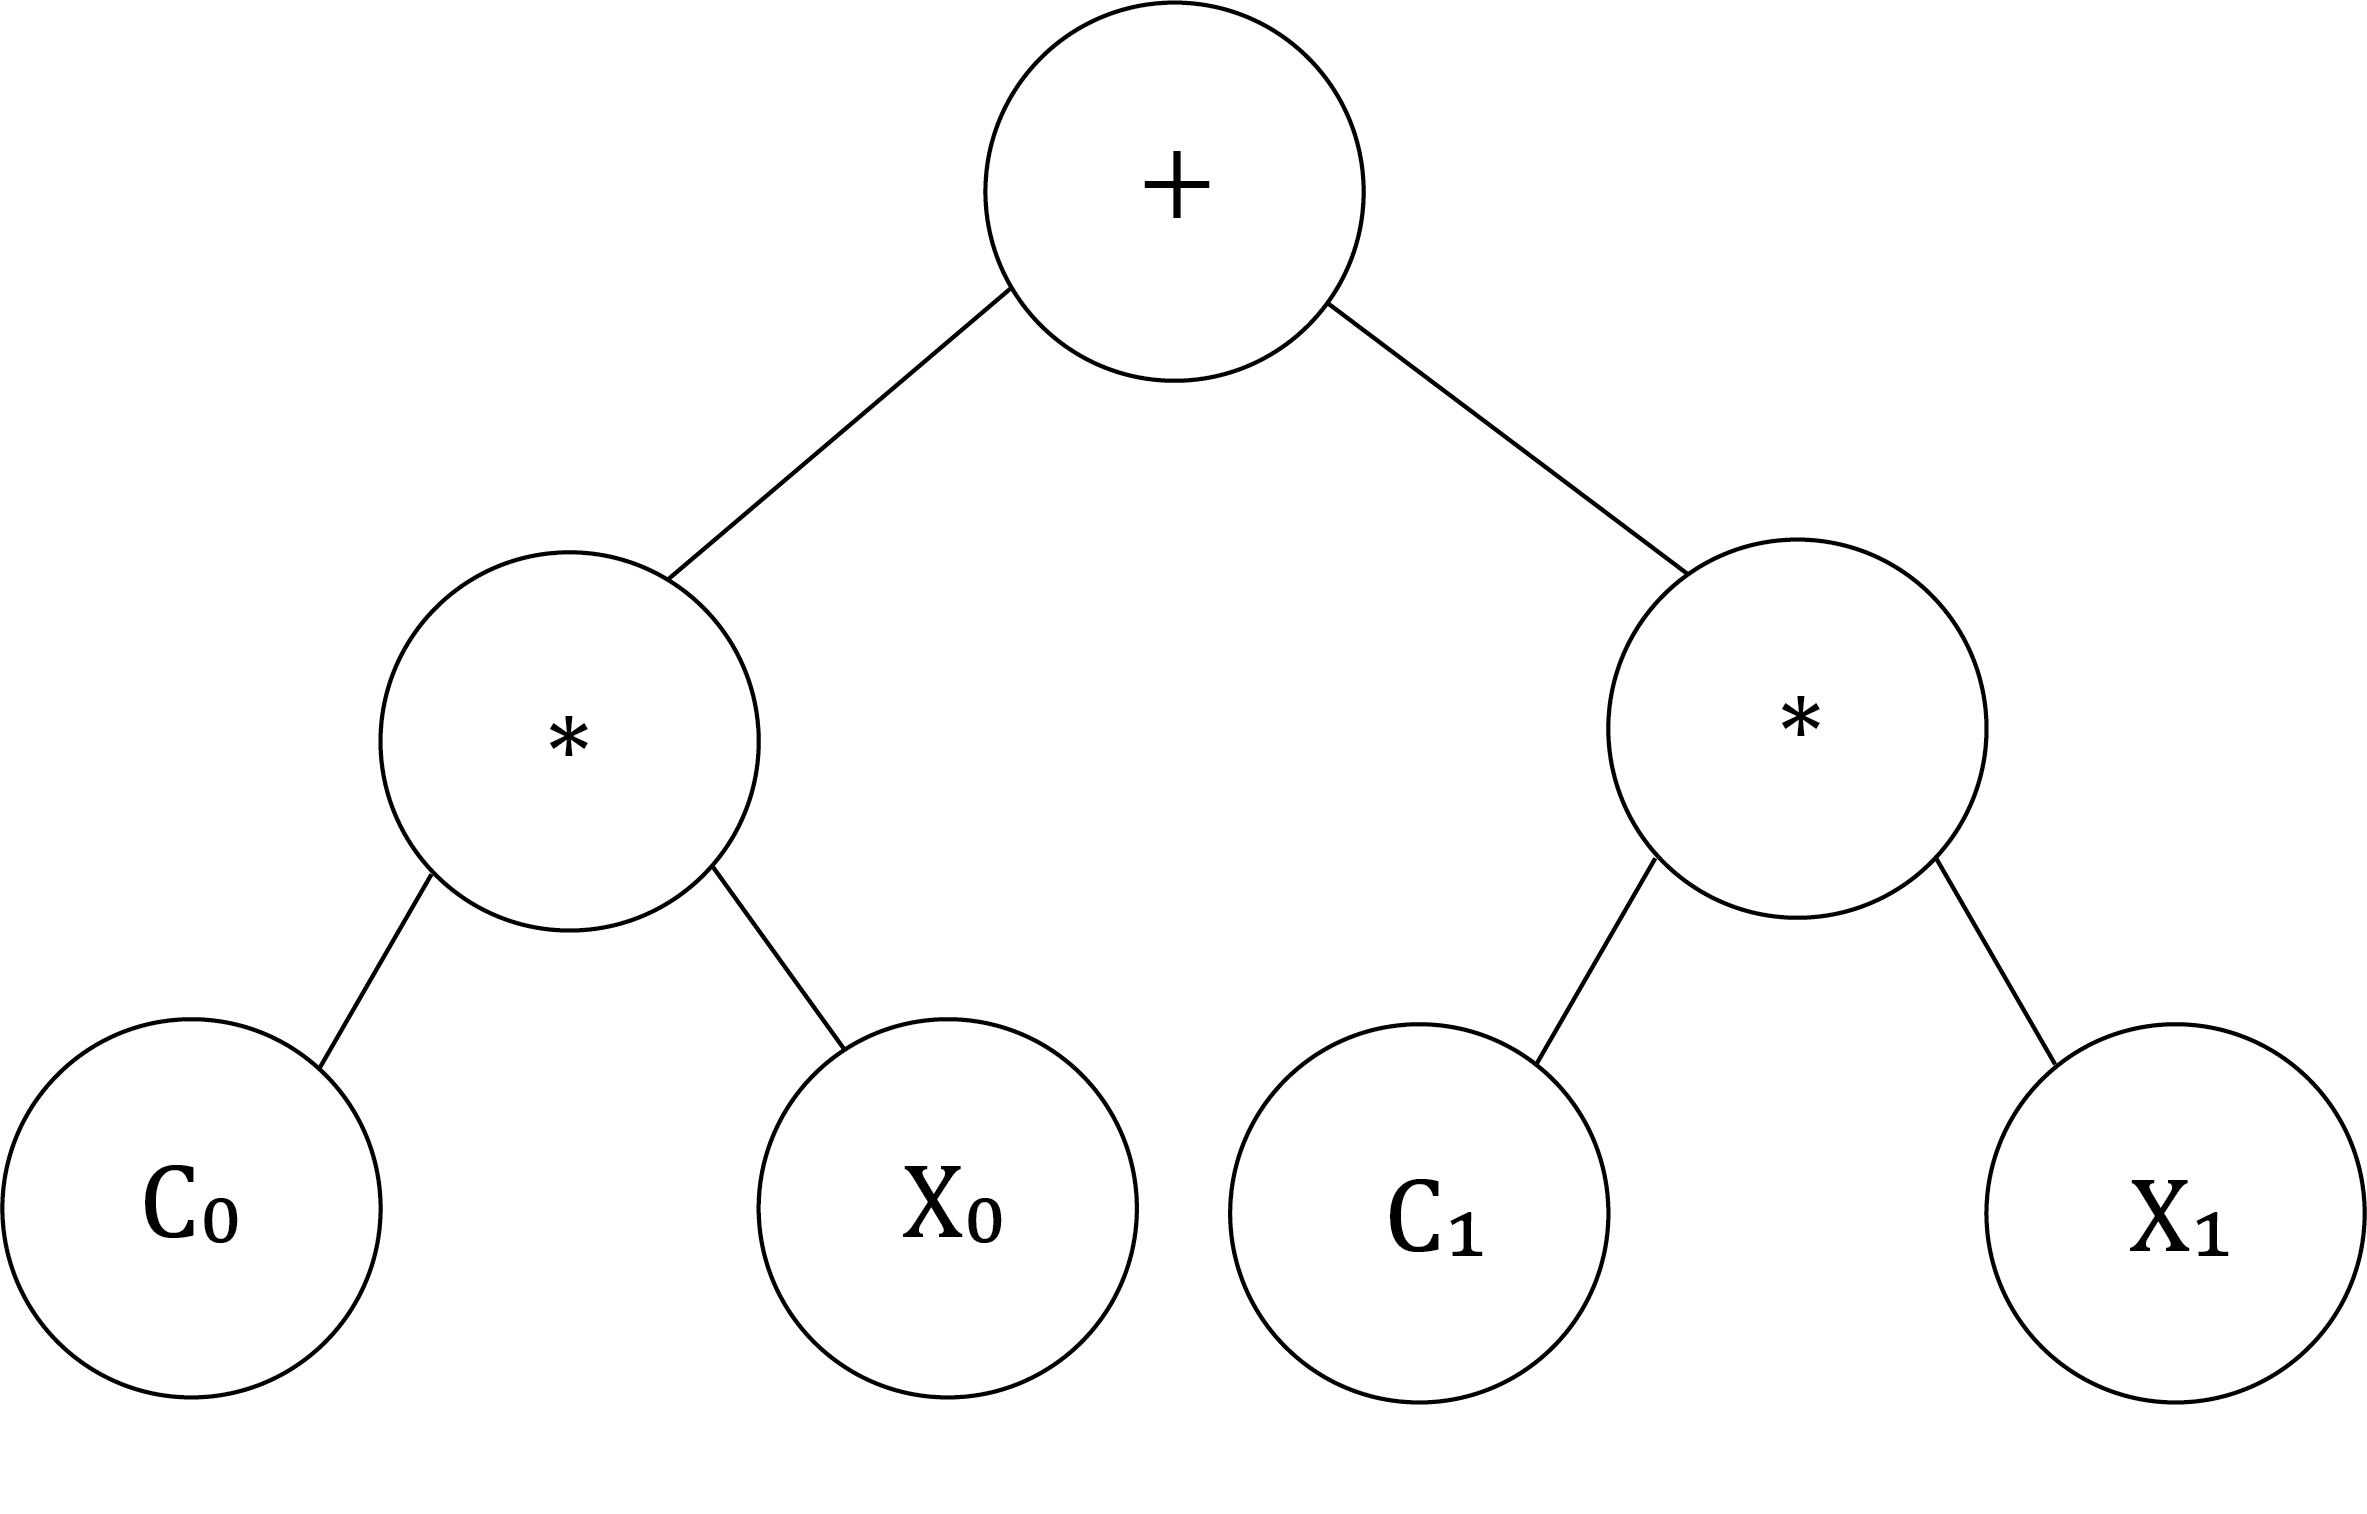
\includegraphics[width=0.6\textwidth]{geometry_figures/agraph.png}
    \label{fig:agraph}
    \caption{Example Agraph for for equation; $C_0 X_0 + C_1 X_1$, where the complexity is the sum of the nodes in this case 7.} 
\end{figure}


\begin{figure}
    \centering

    \begin{minipage}{\textwidth}
        \centering
        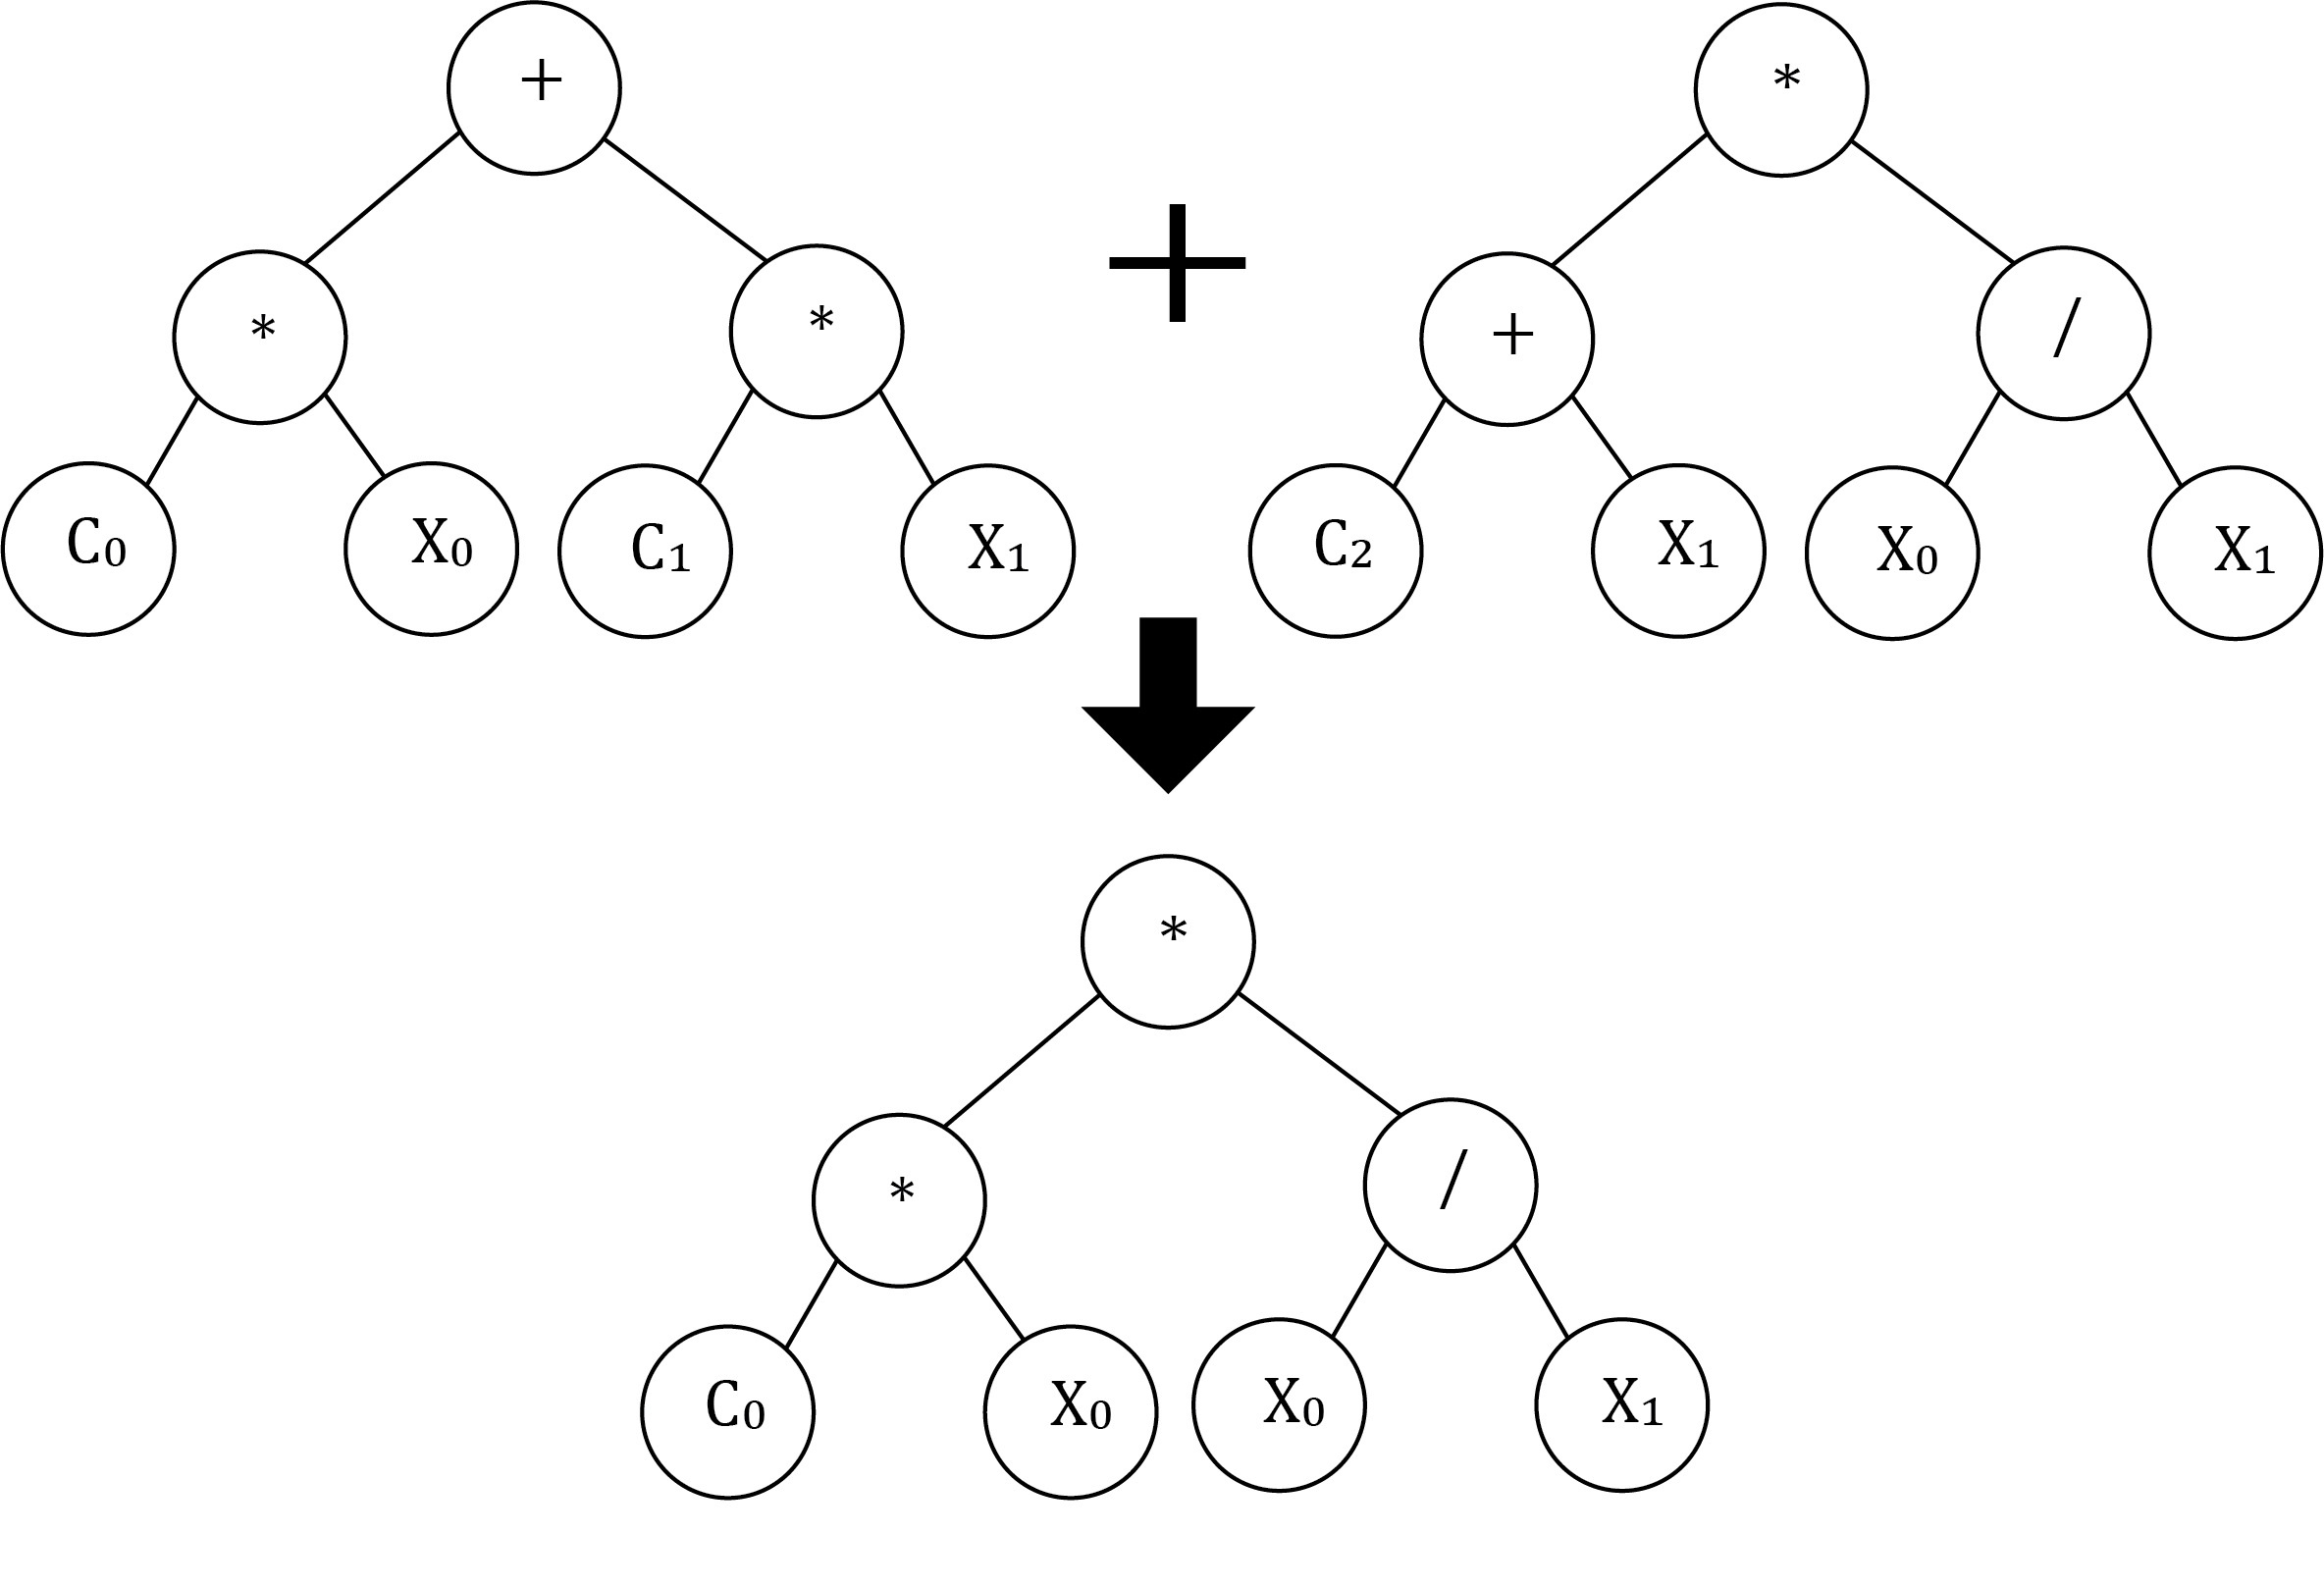
\includegraphics[width=0.8\linewidth]{geometry_figures/agraph-crossover.png}
        \caption*{(a)}
    \end{minipage}
    
    \begin{minipage}{\textwidth}
        \centering
        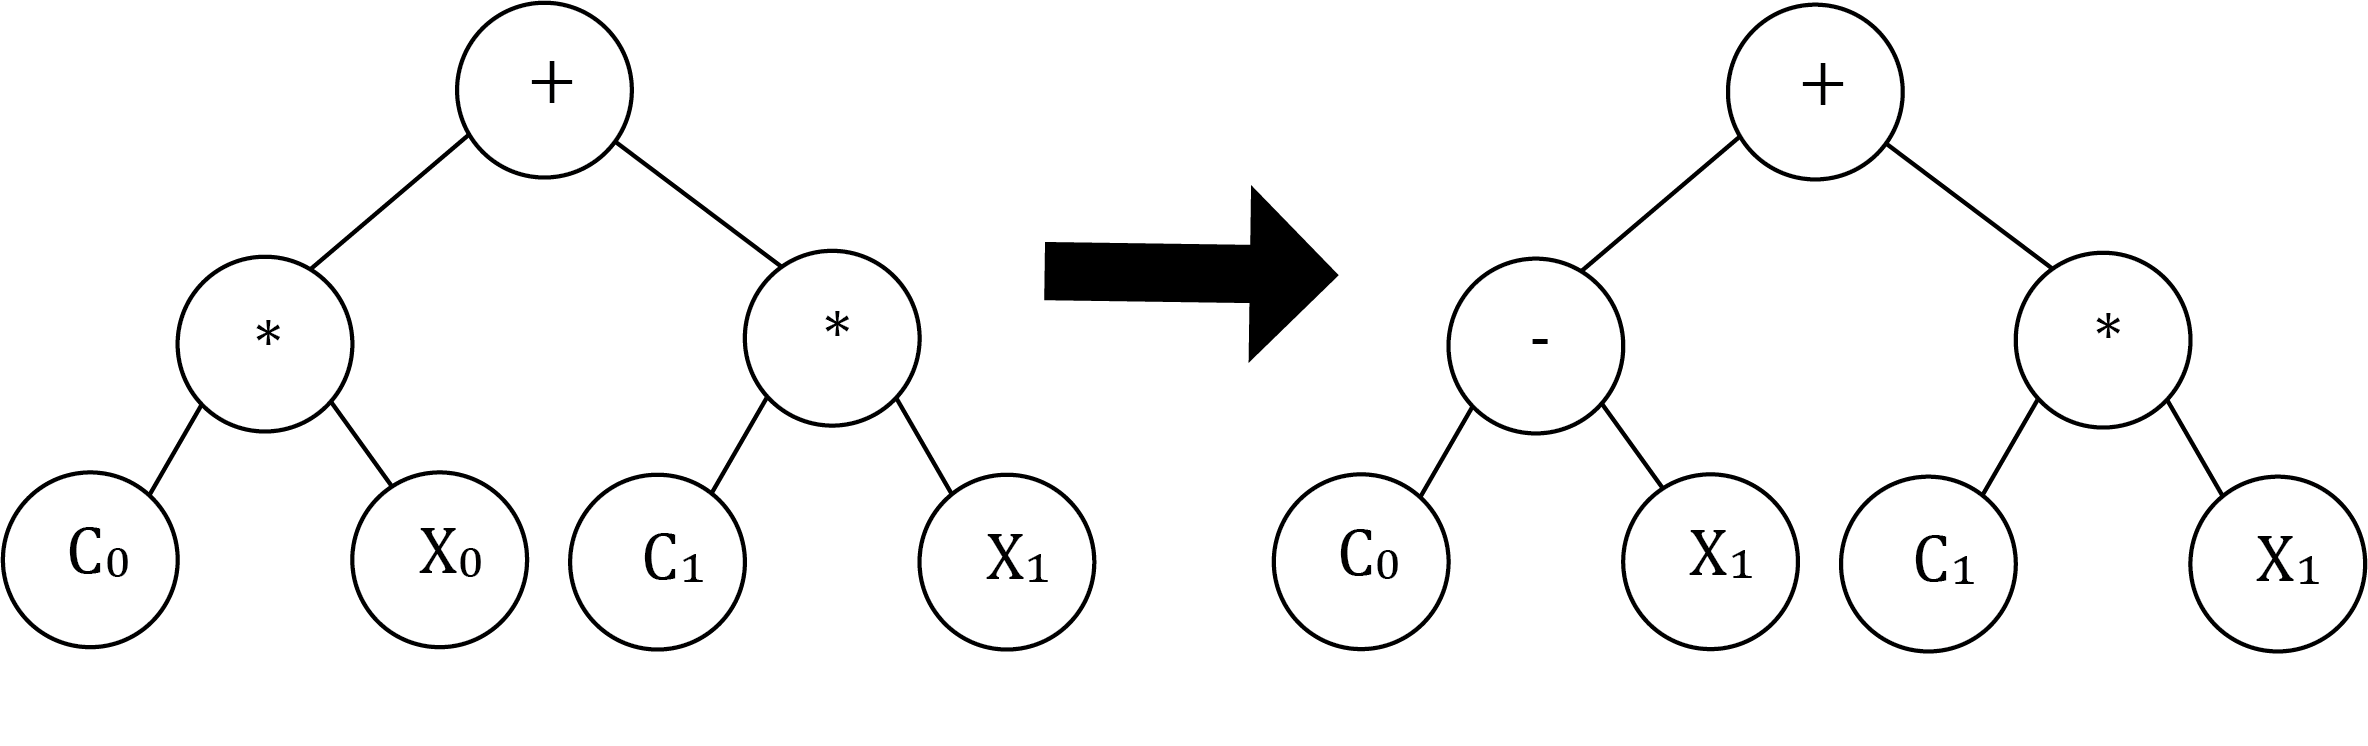
\includegraphics[width=0.8\linewidth]{geometry_figures/agraph-mutation.png}
        \caption*{(b)}
    \end{minipage}
    
    \caption{(a) crossover, where two parent graphs combine features to create a child graph. (b) where part of a graph is randomly changed creating a new graph.}
    \label{fig:agraph_cross_mut}
\end{figure}




The most fit equations, at various complexity values, from the final population are taken and presented as a Pareto front Fig. \ref{fig:perato-front}. Equations with high complexity have better fitness values; however, they often have reduced interpretabiliy from the engineer's perspective. Equations with low complexity tend to be easily interpreteble at the expense of decreased fitness. Lacking additional criteria, a user must decide what equation is the best for the application. Typically, there is a point at which increasing the complexity yields little gain on fitness Fig. \ref{fig:perato-front}, which serves as a balance between accuracy and complexity. ***anotate plot****

\begin{figure}
    \centering
    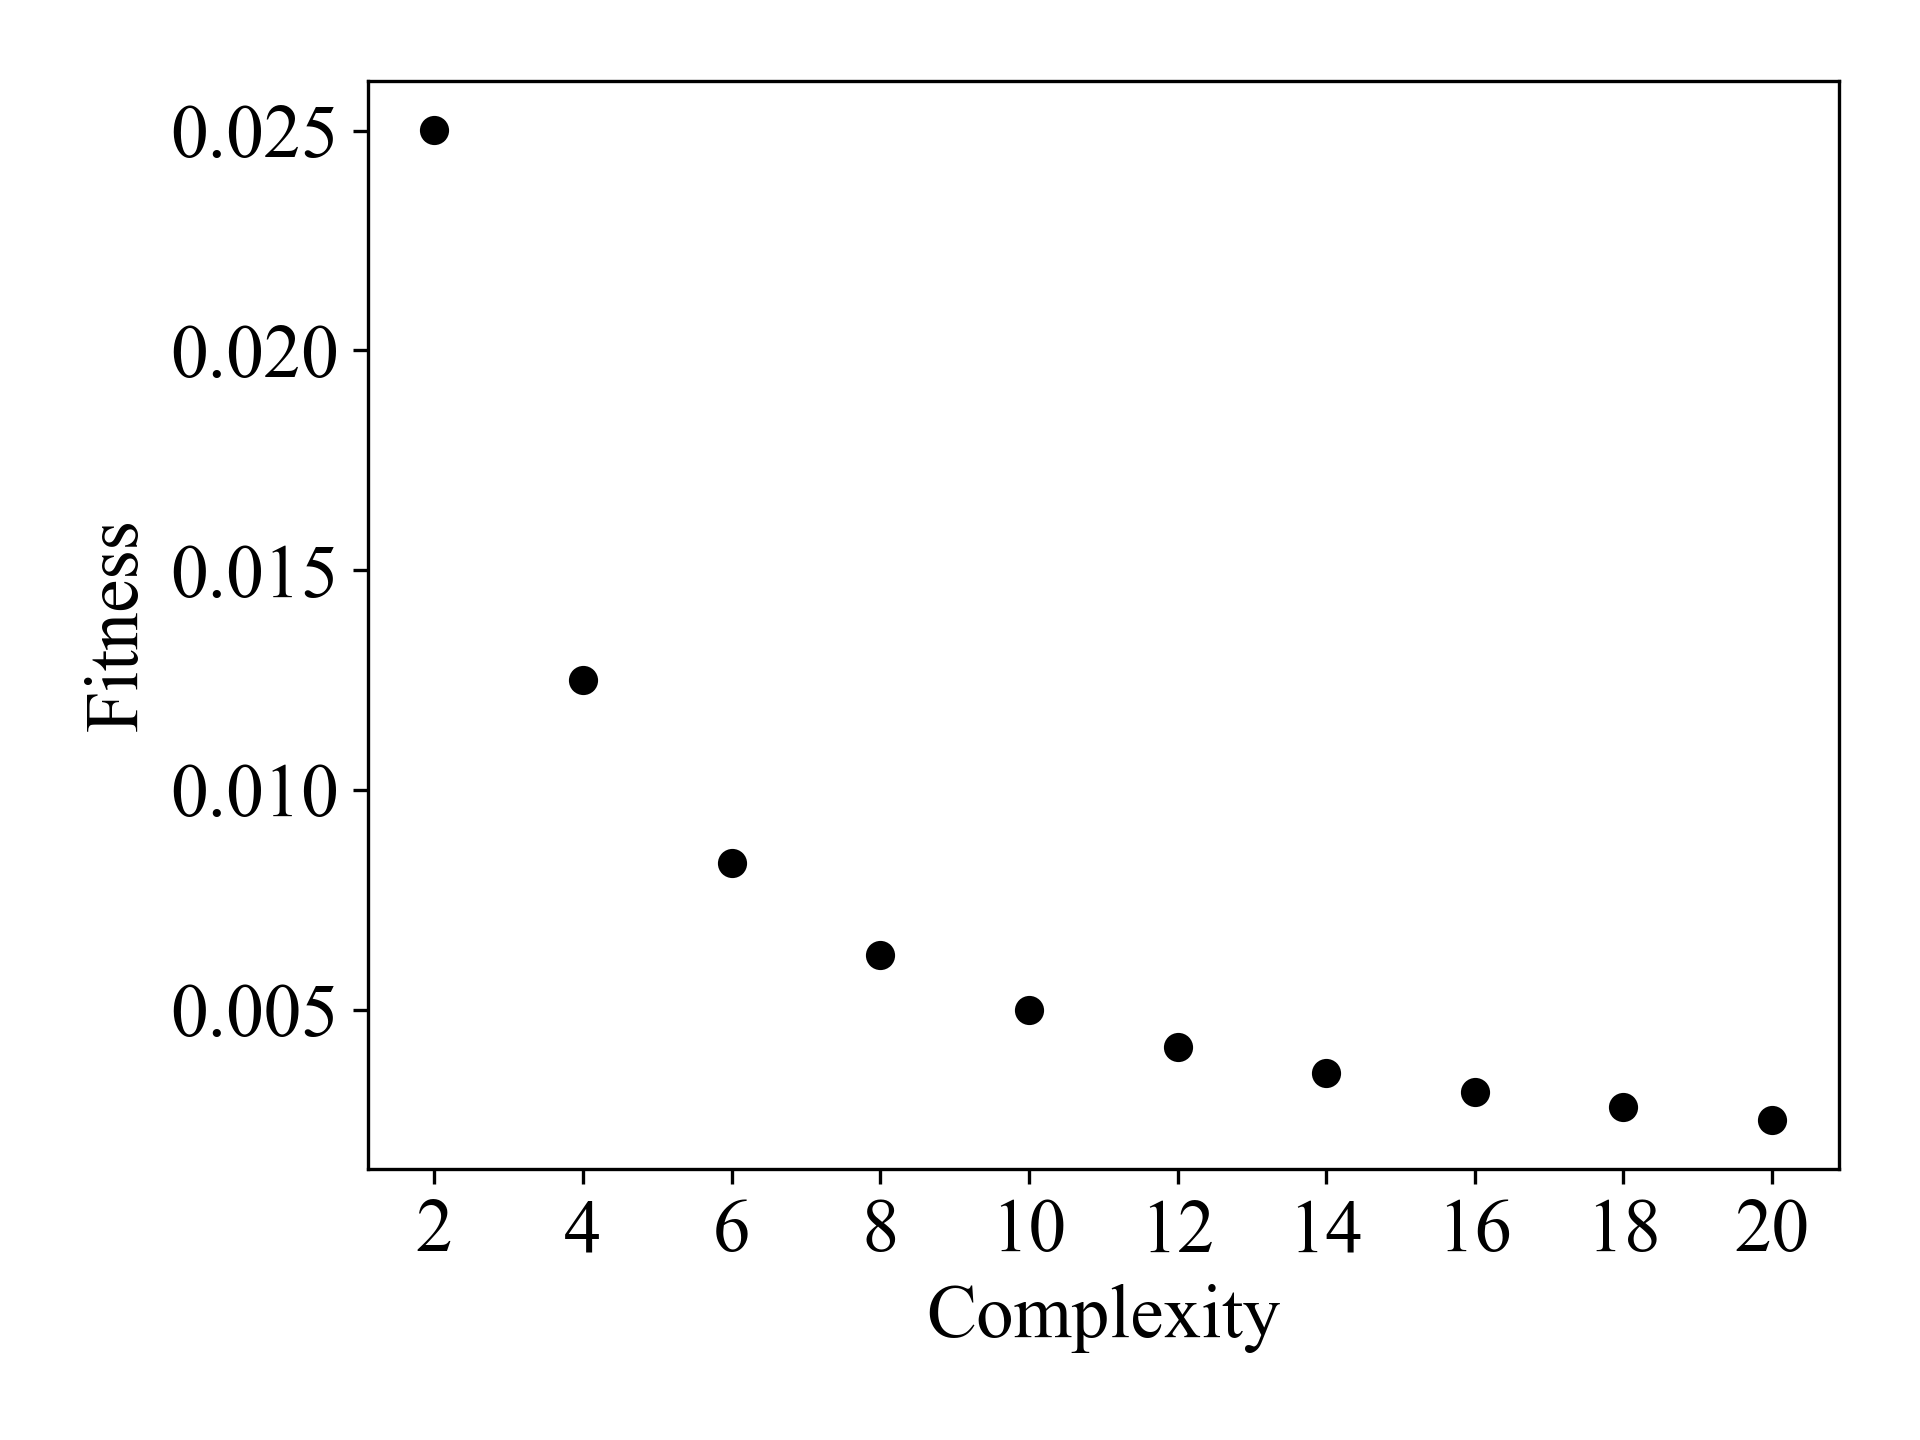
\includegraphics[width=0.6\textwidth]{Figures/dummy_pareto_front.png}
    \label{fig:perato-front}
    \caption{Example Pareto front where the horizontal axis is the model complexity and the vertical axis is the model fitness. Each point on the graph represents a different model in the population.} 
\end{figure}




 
\section{Numerical Experiments}



\subsection{Training Data Generation}

The finite element models were designed to be as consistent as possible with the work presented in \cite{RNeqnsbook}, while using modern computational tools. Using similar boundary conditions (BCs) allows for the comparison between GPSR and the equations created in \cite{RNeqnsbook}. The cracked finite element models are entirely defined by the variables $a$, $c$, $b$, $t$, $h$, and $u$ shown in figure \ref{fig:model_params}. The far field stress $\sigma$ is extracted from the reaction forces at the top and bottom surfaces. The variables $a$ and $c$ are crack parameters and the variables $b$, $t$, and $h$ define the geometry of the plate.

\begin{figure}%
    \centering
    \subfloat[\centering Applied boundary conditions]{{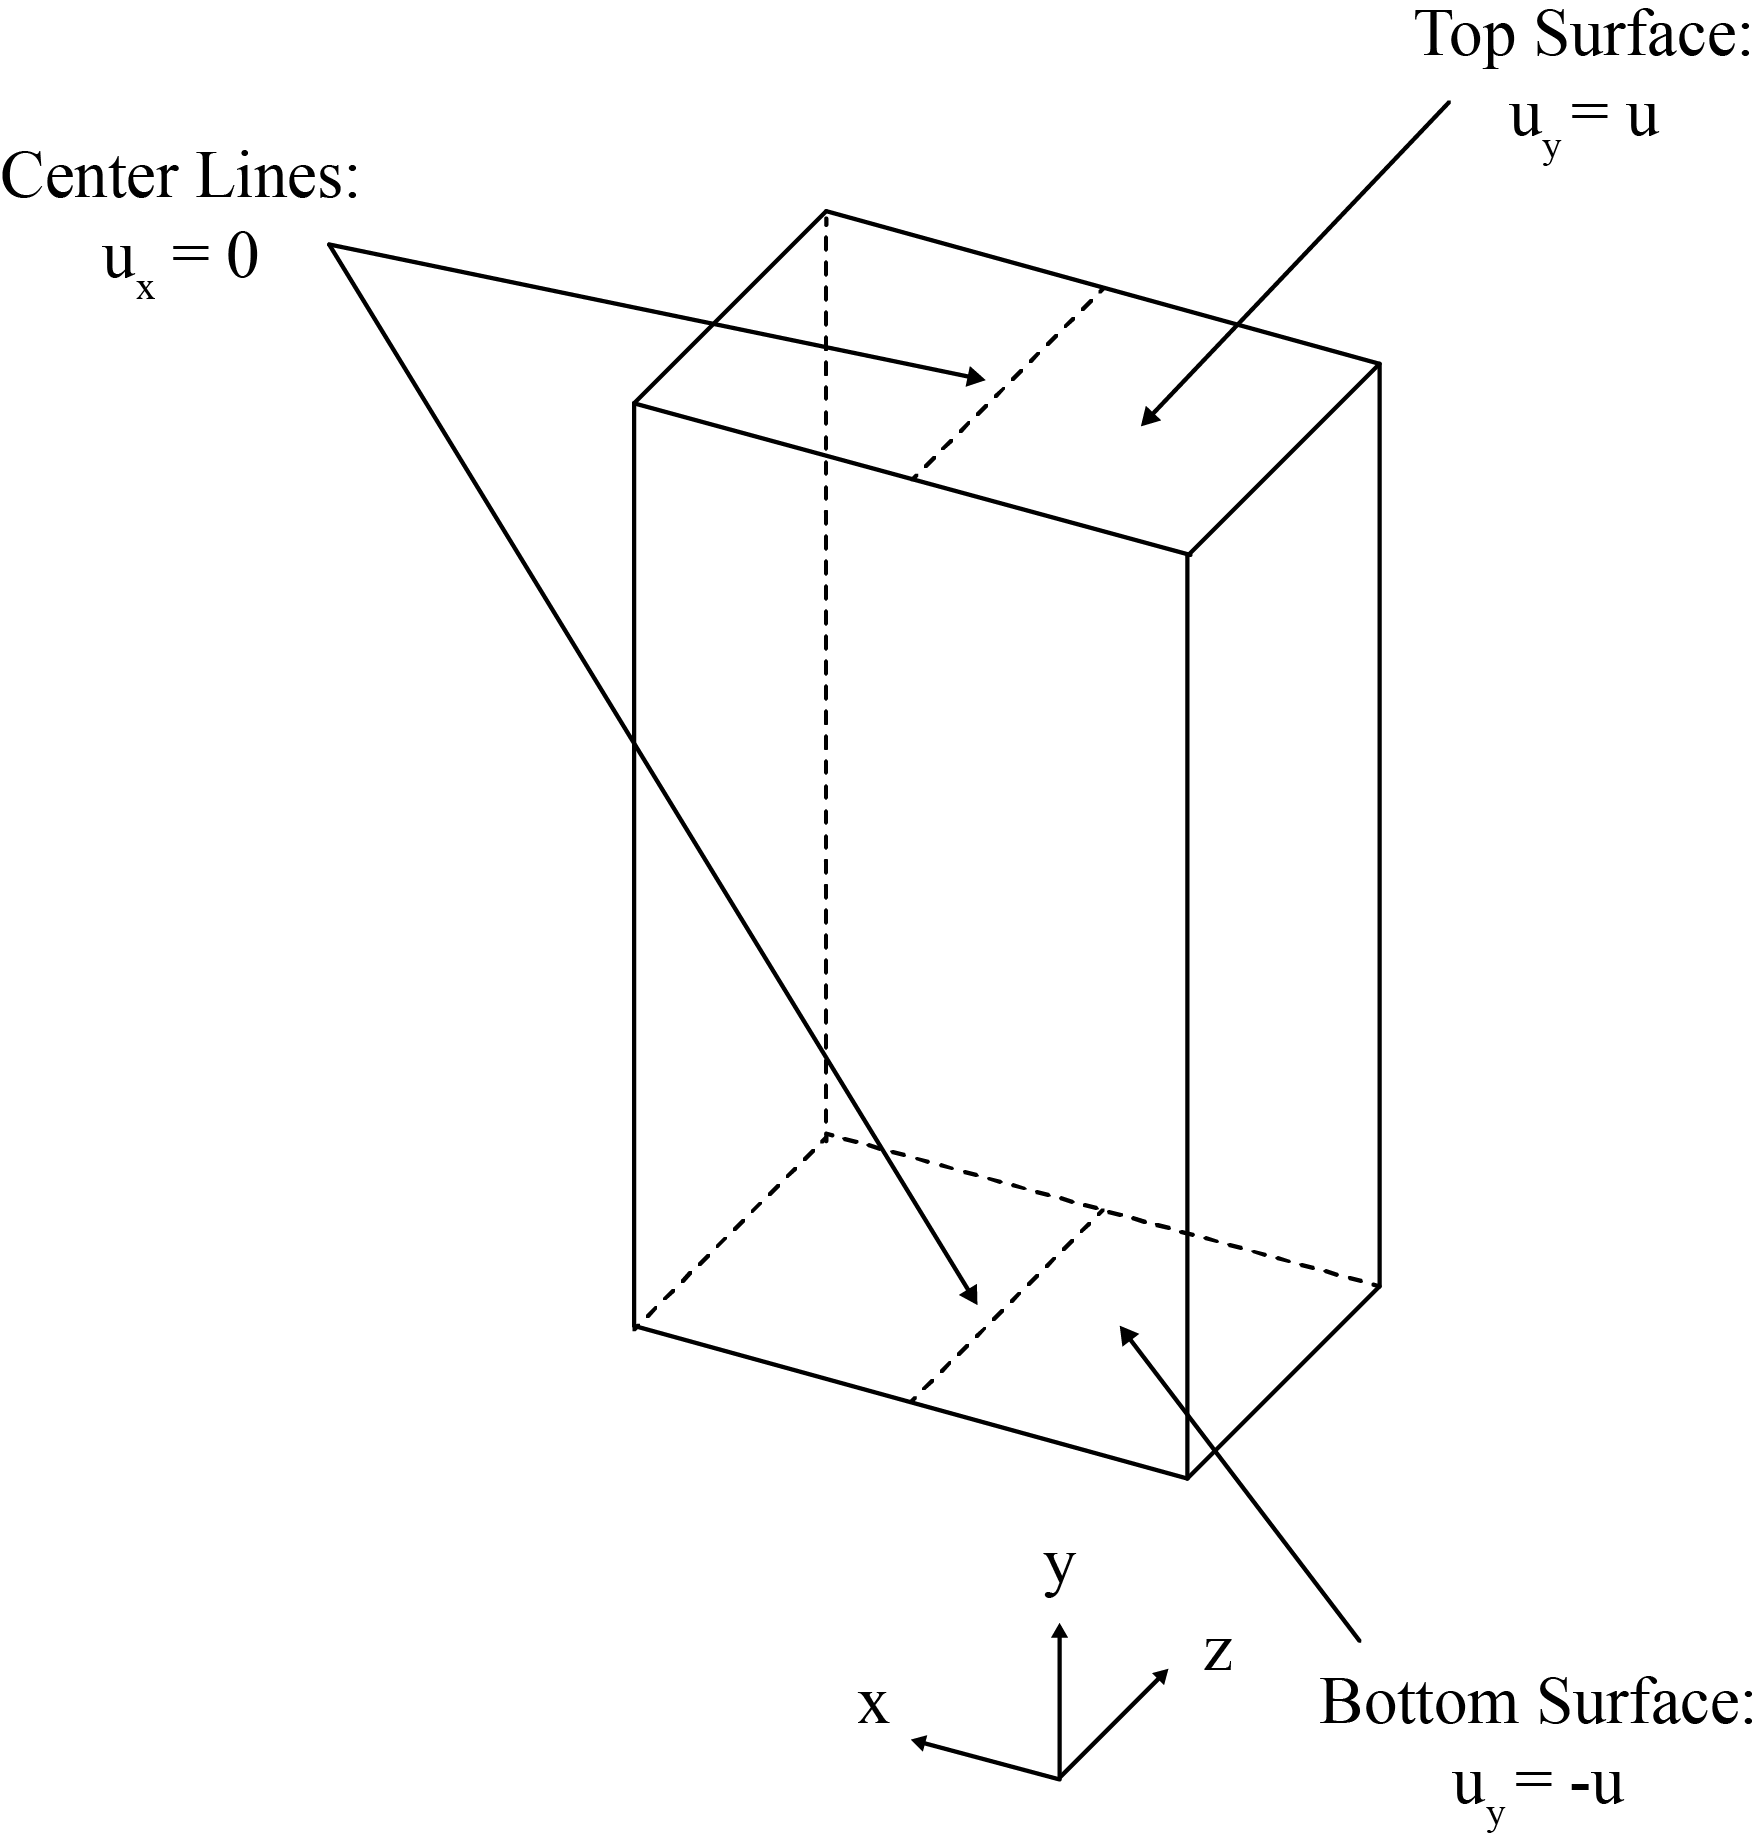
\includegraphics[width=0.6\textwidth]{geometry_figures/BCs.png} }}%
    \qquad
    \subfloat[\centering Model geometry]{{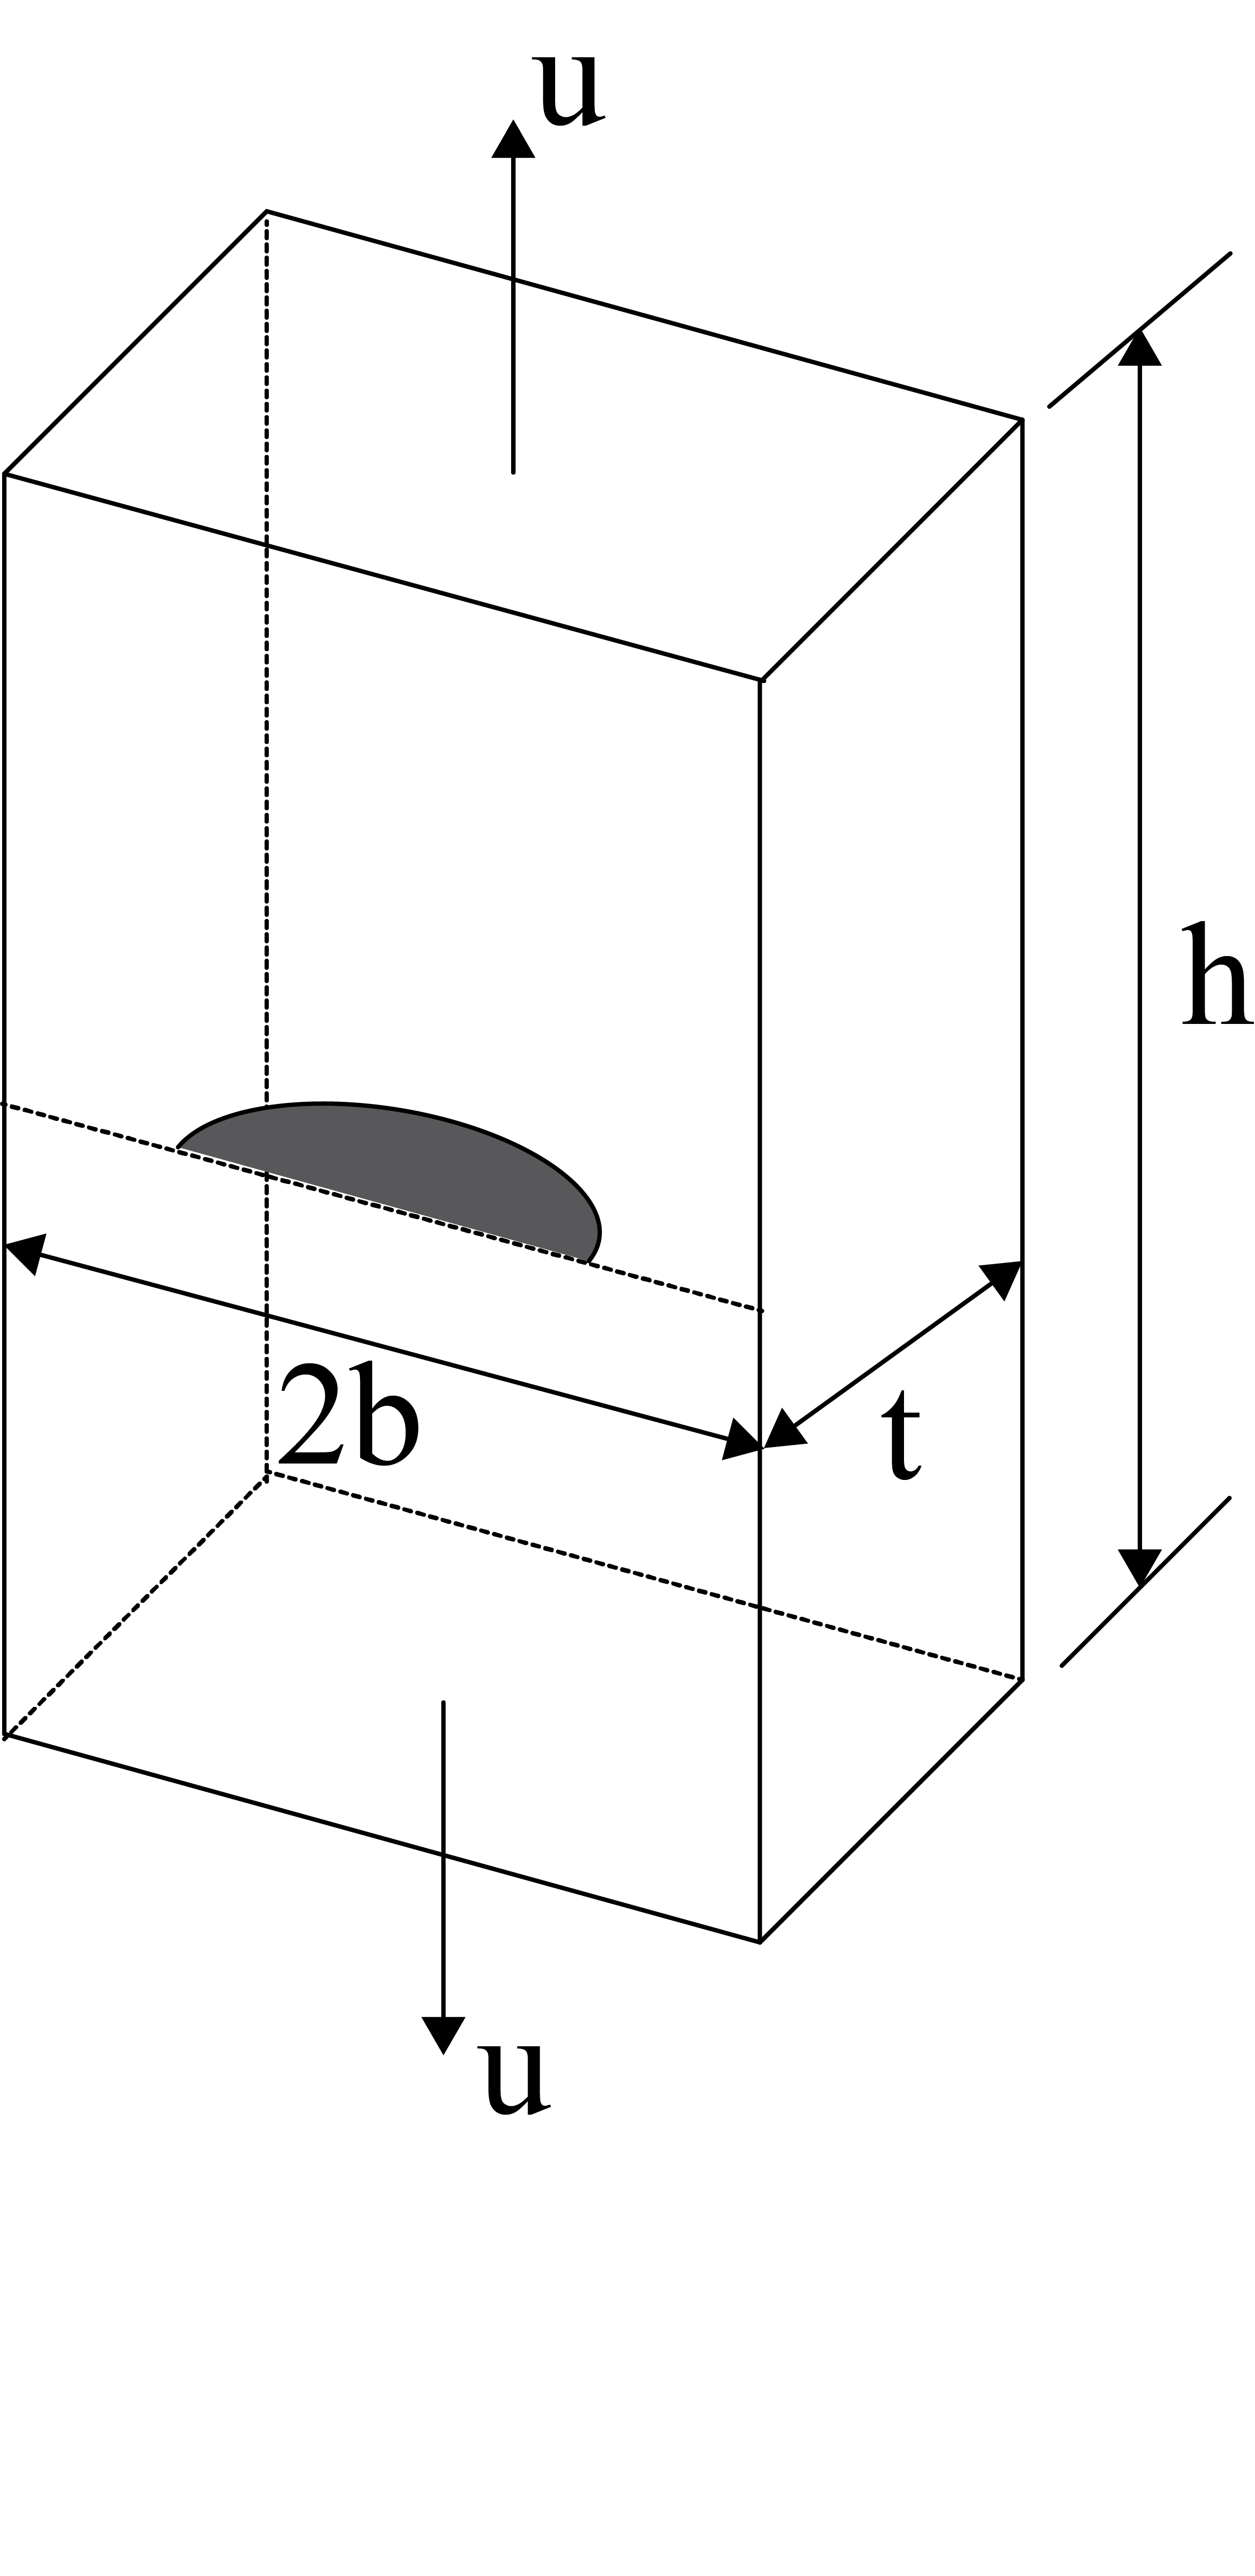
\includegraphics[width=0.3\textwidth]{geometry_figures/Geom.png} }}%
    \caption{(a) Top and bottom surfaces with displacement in $+y$ and $-y$ respectively. The center lines of the top and bottom faces are held $0$ in $x$. (b) Model geometry plate hight: $h$, plate width: $2b$, and plate thickness: $t$.}%
    \label{fig:model_params}%
\end{figure}
	
%uncracked model
In \cite{RNeqnsbook}, Raju and Newman neglected effects due to finite height by assuming the height of the plate to be large relative to the thickness of the plate. To be consistent with this assumption, a constant value of $h/t = 64$ was chosen to remove any effects due to the height of the plate as shown in figure \ref{fig:h_convergence}. As stated previously the BCs of the models were made to match the models from \cite{RNeqnsbook} without overly constraining the model as depicted in figure \ref{fig:model_params}. A constant displacement of $u = 0.001$ units was applied on the top and bottom surfaces in the direction of the surface normals. Additionally the center-lines of the top and bottom surfaces were held fixed in the x-direction to removed rigid body motion. 
\begin{figure}
    \centering
    \subfloat[\centering Convergence of $h/t$]{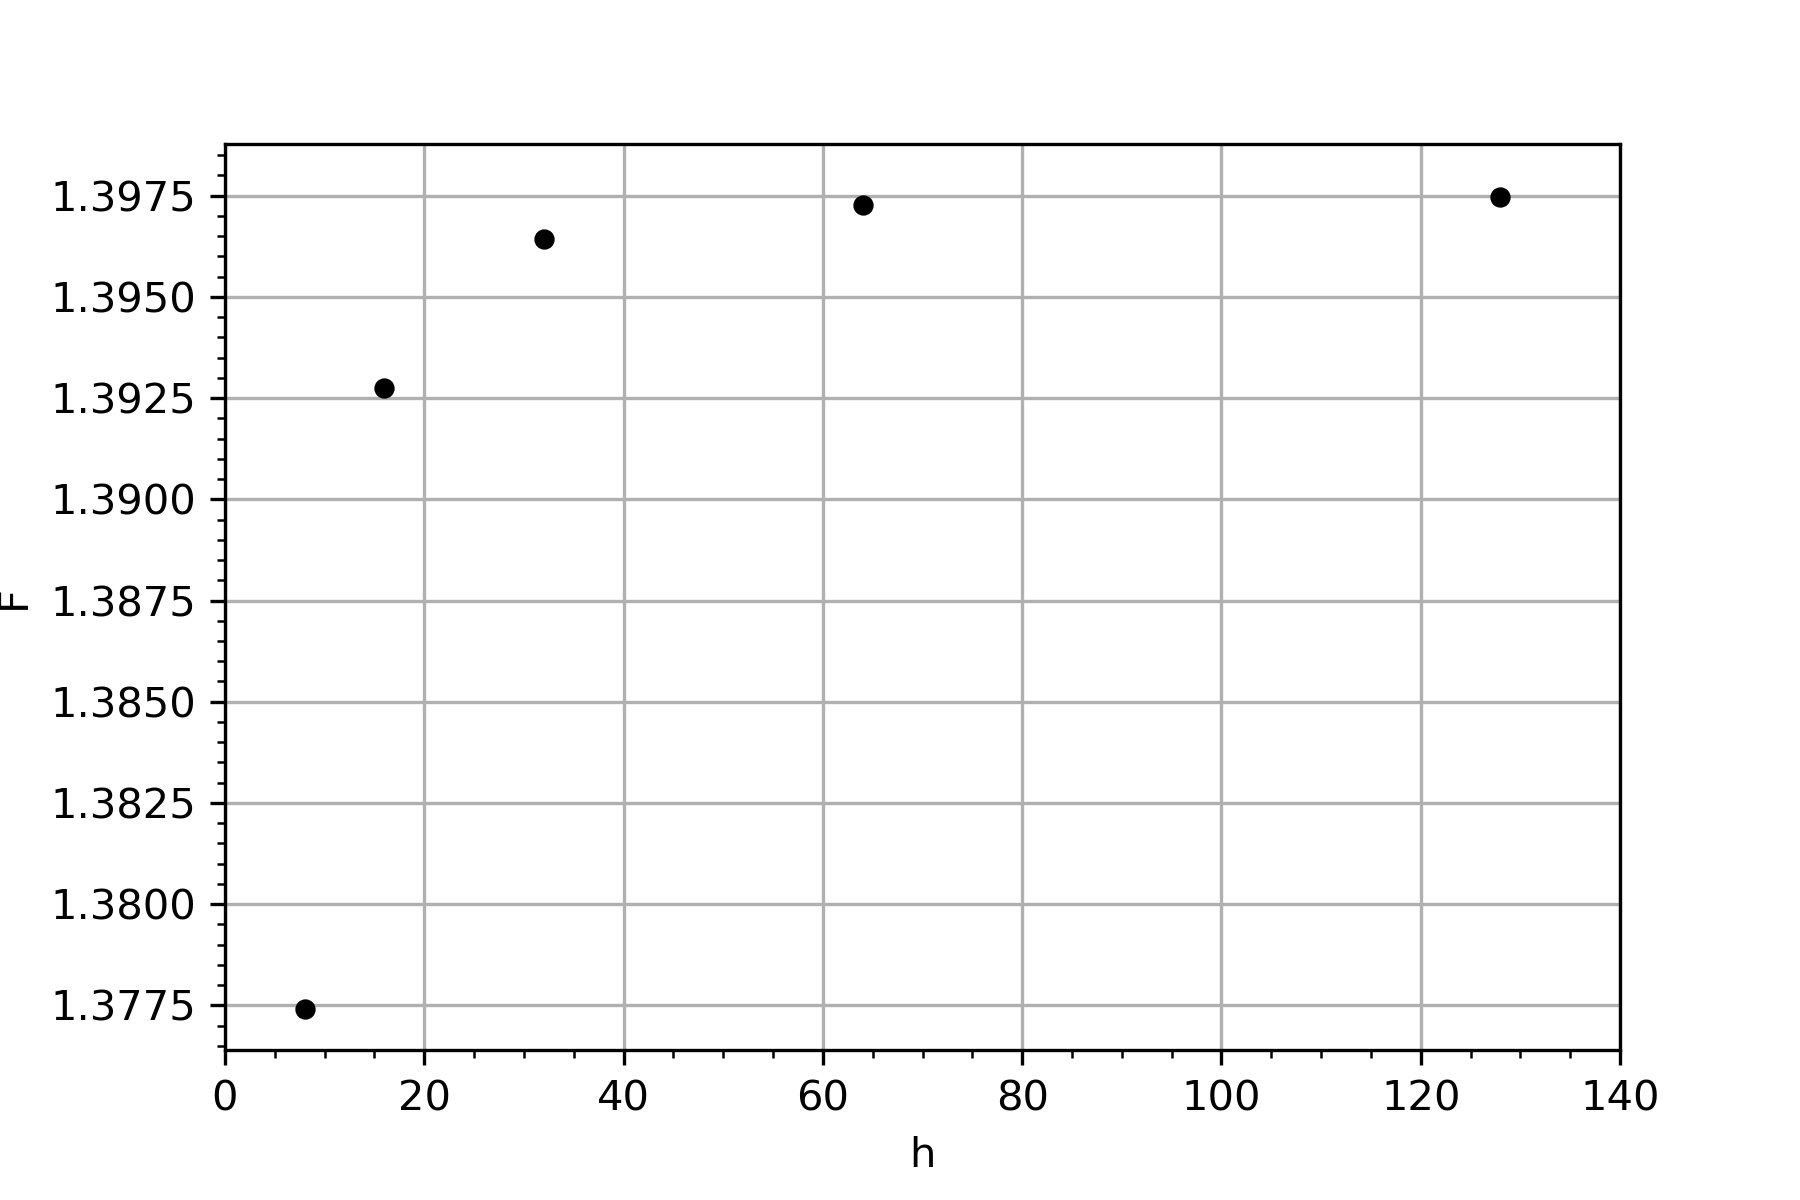
\includegraphics[width=0.45\textwidth]{Figures/h_convergence.png}\label{fig:h_convergence}}%
    \qquad
    \subfloat[\centering Convergence of $c/b$]{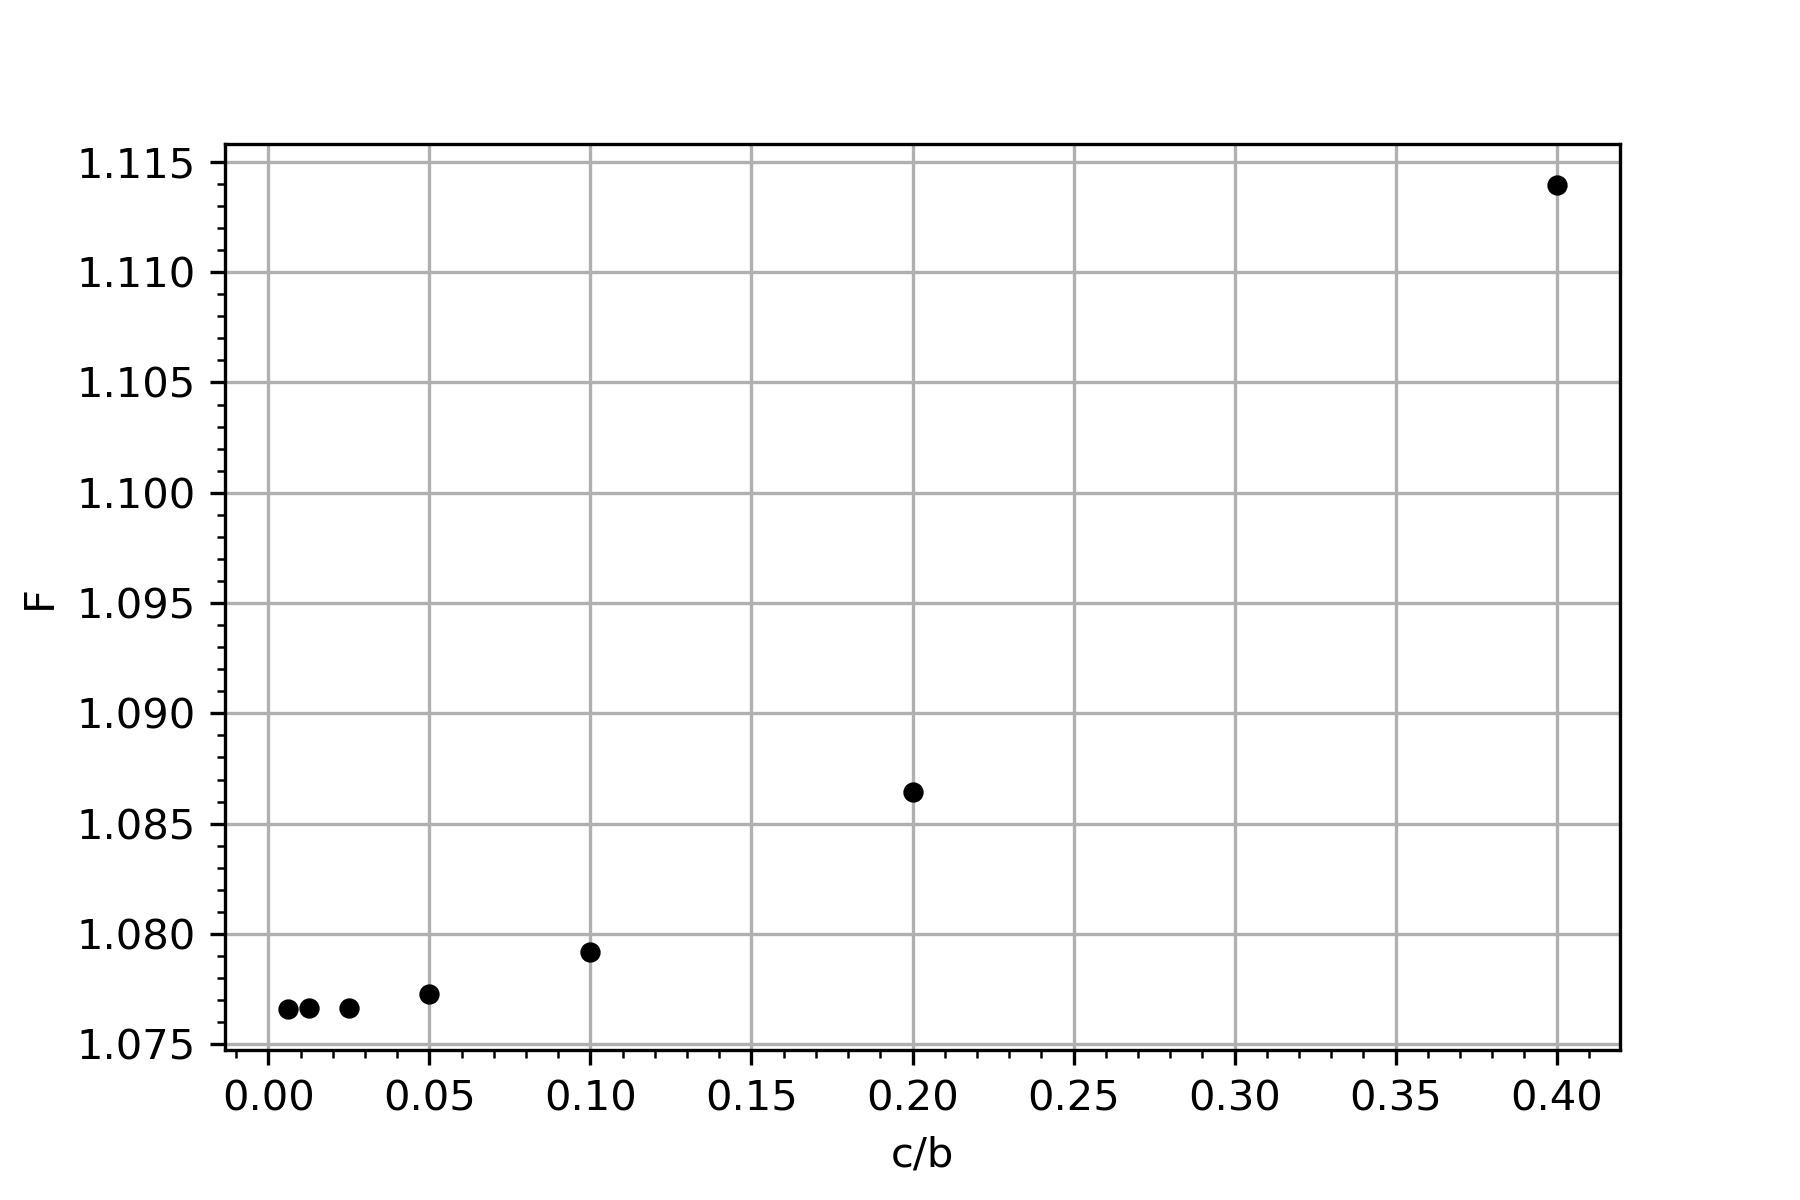
\includegraphics[width=0.45\textwidth]{Figures/cb_convergence.png}\label{fig:cb_convergence}}
    \caption{(a) The convergence of $h/t$ is plotted using the mean boundary correction factor. (b) The convergence of $c/b$ is plotted using the mean boundary correction factor.}
    \label{fig:convergence_plots}
\end{figure}

\begin{table}[]
\centering
\begin{tabular}{|l|l|l|l|}
\hline
\textbf{Feature} & \textbf{min} & \textbf{step} & \textbf{max} \\ \hline
a/c              & 0.2          & 0.05          & 2            \\ \hline
a/t              & 0.2          & 0.05          & 0.8          \\ \hline
c/b              & 0.01         & 0.05          & 0.4          \\ \hline
$\phi$           & 0            & $\pi / 150$  & $\pi$        \\ \hline
\end{tabular}
\caption{Max and min values for each of the features used when creating the cracked FE models}
\label{table:feat_range}
\end{table}


The crack mesh created by FRANC3D is shown in \ref{fig:f3d_crack}. The mesh contains a ring of quarter points elements around the crack front followed by rings of brick elements. The parameters for the crack mesh are the template radius which specifies the size of each element; the number of rings of elements around the crack; and the number of circumferential elements in each ring. Instead of using a fixed template radius a number of elements along the entire crack was specified. This produced better results with varying crack aspect ratios. The best SIF values were computed with 300-600 elements along the crack, 8 rings of elements, and 14 circumferential elements per ring as shown in table \ref{table:optimized_vals}. The average SIF value for each model is relatively insensitive to the crack mesh, however certain crack geometries display numerical noise for certain crack mesh sizes as shown in figure \ref{fig:crack_mesh_convergence}. The models that displayed the most numerical noise for the most crack sizes were the models with values close to the following: $a/c = 0.5$, $a/t = 0.6$, and $c/b = 0.2$. The crack mesh parameters were chosen based off of these models and then applied to the rest of the models. Before running the entire data-set, a random sample of 10\% of the total models was computed to check for convergence. After convergence was confirmed on those models the entire data-set was computed. 

\begin{figure}
    \centering
    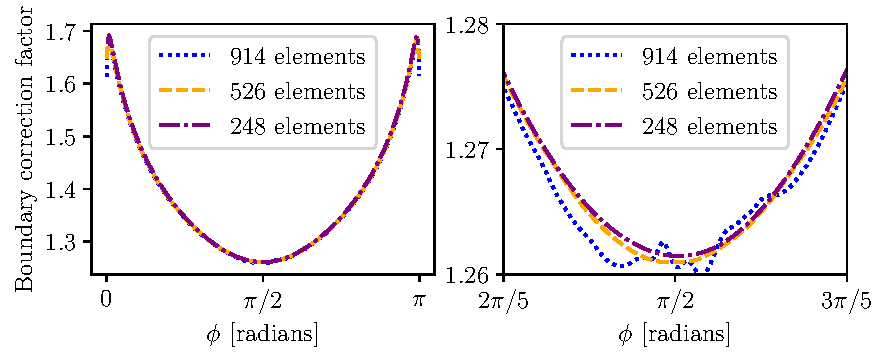
\includegraphics[width=\textwidth]{Figures_pdf/numerical_noise.pdf}
    \label{fig:crack_mesh_convergence}
    \caption{(left) entire SIF plot for differing number of elements along the crack front. (right) plot zoomed in at $\pi/2$ to highlight numerical noise with high element count.}
\end{figure}



The converged values are tabulated in table \ref{table:optimized_vals}
\begin{table}[]
\centering
\begin{tabular}{|l|l|}
\hline
Thickness                   & 1         \\ \hline
h/t                         & 64        \\ \hline
Global seed                 & max(0.25, min(b/50, 0.5))      \\ \hline
Local seed                  & 0.25      \\ \hline
Number of rings             & 8         \\ \hline
Number of circumferential elements             & 14        \\ \hline
Number crack front elements & $\sim$300 \\ \hline
\end{tabular}
\caption{Optimized model and mesh values}
\label{table:optimized_vals}
\end{table}




After the converged model parameters were found all 2500 of the models were run to calculate 300-450 SIFs per model. Figure \ref{fig:selected_sifs} shows the calculated SIF values from a few of the models compared to the SIFs calculated from \cite{RNFEM}.  

\begin{figure}
    \centering
    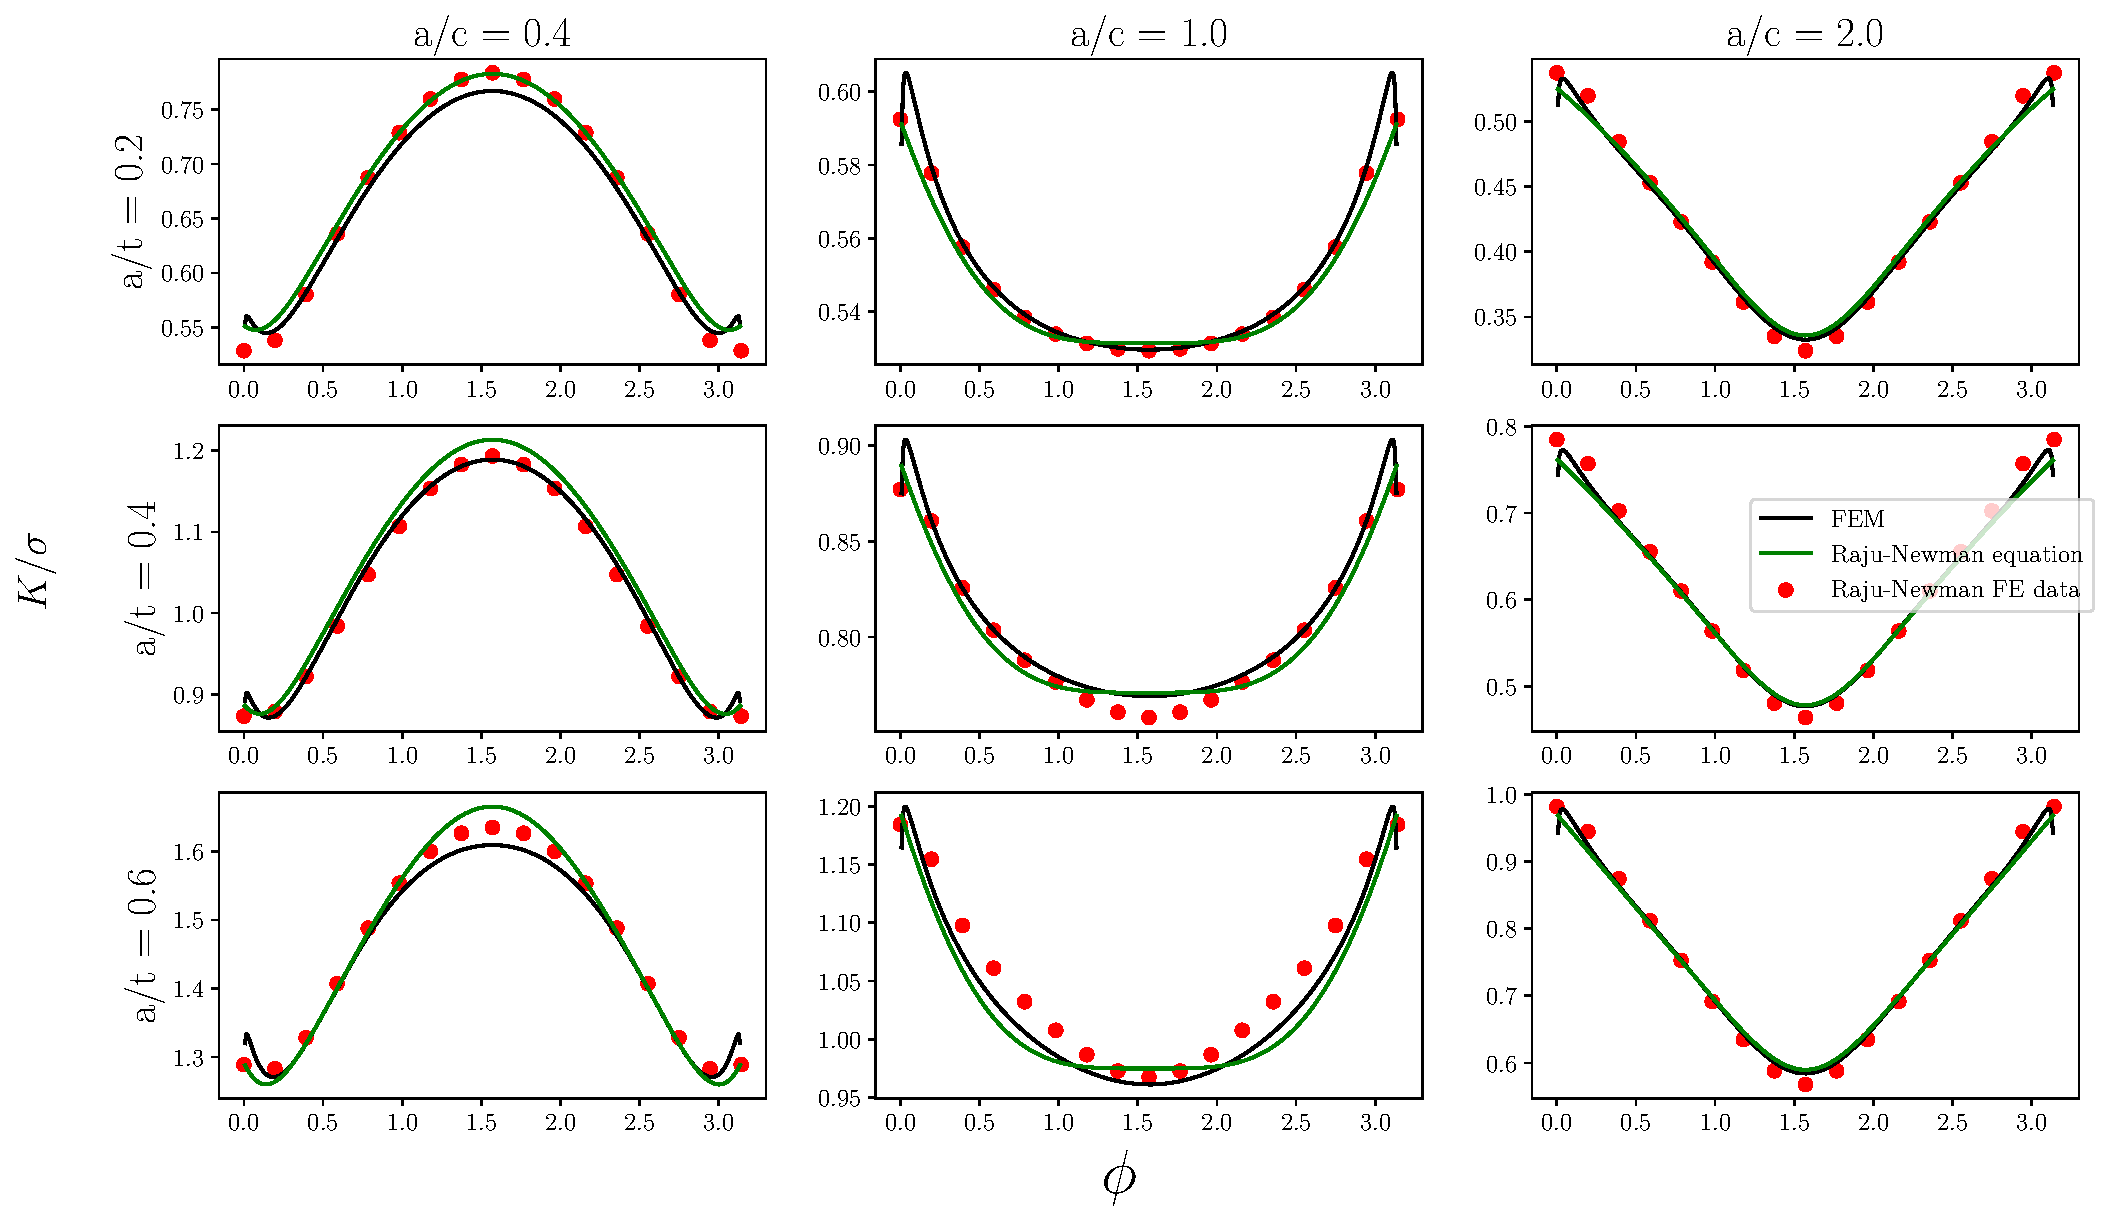
\includegraphics[width=\textwidth]{Figures_pdf/K_data.pdf}
    \label{fig:selected_sifs}
    \caption{SIF values from a selection of models plotted with the Raju-Newman equation.}
\end{figure}

%%%%%%%%%%%%%%%%%%%

\subsection{Training Data Subdivision}

The 2500 models were used for training and model selection, While a additional isolated set of 400 models were generated for testing to allow for better generalization error predictions. Instead of directly training on the SIF data extracted from FRANC3D this paper uses a mechanics based approach to simplify the training process which increases the explainablity of the final SIF model. The approach used in \cite{RNeqnsbook} was used to break the model for $K$ into two parts: the known part and the learned part. The known part includes equation \ref{eqn:K_embedded_ellipse}, which is the solution to the embedded ellipse in an infinite volume. The learned part of the equation is the boundary correction factor which is comprised of three sub-functions $f_w$, $M$, and $g$ each accounting for a different deviation from the infinite case. The finite width correction factor $f_w$ accounts for the effect of finite width and thickness at the center of a semi-circular crack. The $M$ equation expands on $f_w$ by accounting for the aspect ratio of the crack. The two functions $f_w$ and $M$ together comprise the boundary correction factor for the center of a semi-elliptical crack in a finite plate. Finally the $g$ equations takes this correction at the center and applies it to the rest of the crack allowing for SIFs to be predicted along the entire length of the crack. GPSR is especially suited for this process as it finds closed form equations which can conform exactly to the known limits of each of the boundary correction terms significantly increasing interpretability.

Two modifications were made to the approach used in \cite{RNeqnsbook} to make the training process easier and the resulting models more interpretable. The first is the method to modify the embedded ellipse equation to allow for $a/c > 1$. This was done by using the function $l$ from \cite{tada1985} and modifying it to allow for  $a/c > 1$ as shown in equation \ref{eqn:l}


\begin{equation} \label{eqn:l}
l = a \left( \frac{c}{\alpha} \right)^2 \sqrt{\left( \frac{a}{c} \right)^2 \cos^2 \phi + \sin^2 \phi},
\end{equation}

where $a$ is the crack depth, $c$ is half-crack surface length, and $\alpha$ is the length of the major axis of the ellipse. The function $l$ is a sort of pseudo radius which is a measure of the perpendicular distance from the tangent line at the point of interest to the nearest axis seen in figure \ref{fig:crack_params}. The benefit of modifying the embedded ellipse equation by using equation \ref{eqn:l} is that it removes the need for any piece-wise functions (like those use in \cite{RNeqnsbook}), as the that is all handled by the variable $\alpha$. This reduces the number of models that have to be trained from five as in \cite{RNeqnsbook} to three, one for each of $f_w$, $M$, and $g$. This reduces training time and lowers the complexity of the final $K$ solution resulting in a more interpretable equation. 

The second modification is the formulation of $f_w$, while Raju and Newman used a 3D modification of a finite width correction factor for a 3d through crack from \cite{brown1966}, this work will create a finite width correction factor specifically for the case of a semi-elliptical surface crack. To be able to use the process outlined in \cite{RNeqnsbook} The $f_w$ function was created as similarly as possible to the one use by Raju and Newman in order to be able to use their method of breaking down the equation. This means that $f_w$ will still be a finite width and thickness correction when $\phi = \pi/2$ and $a/c = 1$. 

When $\phi = \pi/2$ and $a/c = 1$ the value of $K$ converges to the embedded ellipse equation as $a/t$ and $c/b$ go to zero as seen in figure \ref{fig:fw_convergence}. This results in $f_w$ being defined as equation \ref{eqn:fw_parameter_def}

\begin{figure}
    \centering
    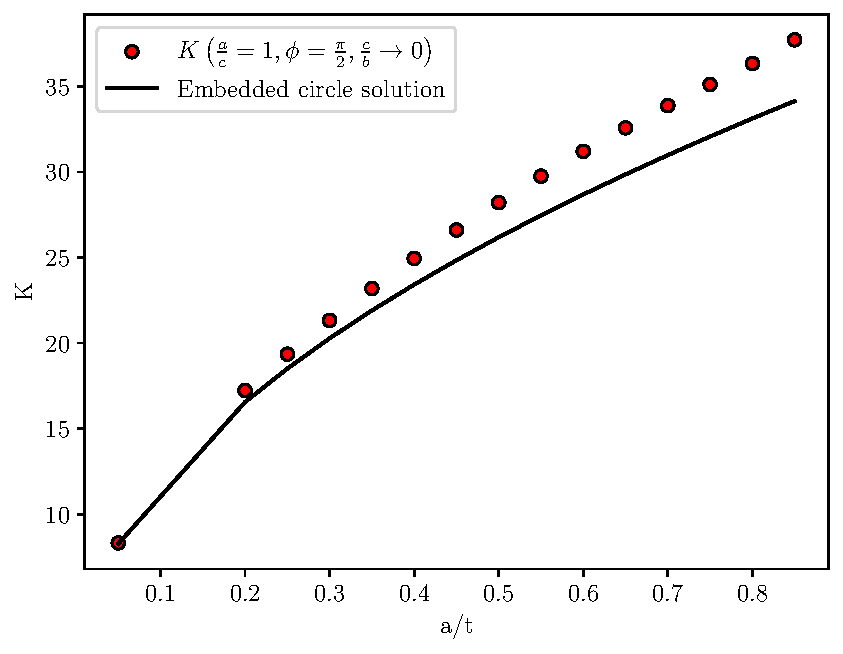
\includegraphics[width=\textwidth]{Figures_pdf/fw_convergence.pdf}
    \label{fig:fw_convergence}
    \caption{Comparison of K from the center of a surface crack and the solution to an embedded circle crack in an infinite volume as a function of a/t where c/b = 0.01, which has been determined to be close to 0 \ref{fig:convergence_plots}}
\end{figure}


\begin{equation} \label{eqn:fw_parameter_def}
    f_w\left(\frac{c}{b}, \frac{a}{t}\right) = \frac{K\left(\frac{a}{c} = 1, \phi = \frac{\pi}{2}\right)}{\sigma \frac{2}{\pi} \sqrt{\pi a}},
\end{equation}

resulting in $f_w$ correcting for finite width and thickness effects. The final equation for $K$ will be in the form of equation \ref{eqn:K_semi_with_l} 

\begin{equation} \label{eqn:K_semi_with_l}
    K = \sigma \frac{\sqrt{\pi l}}{E} f_w M g,
\end{equation}

where $f_w$, $M$, and $g$ are the boundary correction functions learned by Bingo and $\sigma \sqrt{\pi l}/E$ is the modified embedded ellipse solution. 


The process of extracting the training data from the SIF data calculated from the FE models is outlined here.
\begin{equation} \label{eqn:K_parameter_def}
    K\left(\frac{a}{c}, \frac{a}{t}, \frac{c}{b}, \phi, \sigma \right) = K_{ee} \left(
\frac{a}{c}, \sigma, \phi \right) f_w \left(\frac{a}{t}, \frac{c}{b} \right) M \left(\frac{a}{t}, \frac{a}{c} \right) g \left(\frac{a}{t}, \frac{a}{c}, \phi \right)
\end{equation}

The process of calculating the $f_w$ training data was previously shown in equation \ref{eqn:fw_parameter_def}. The next step is to extract the training data for $M$, which is computed similarly to $f_w$. The SIF data from FEA data is taken at $c/b = 0$ and $\phi = \pi/2$ then divided by equation \ref{eqn:K_embedded_ellipse} and equation \ref{eqn:fw_parameter_def} evaluated at $\phi = \pi/2$ resulting equation \ref{eqn:M_parameter_def} that is only a function of $a/c$ and $a/t$. 

\begin{equation} \label{eqn:M_parameter_def}
    M \left(\frac{a}{t}, \frac{a}{c} \right) = \frac{K_{FE}\left(\frac{c}{b} \rightarrow 0, \phi=\frac{\pi}{2}\right)}{f_w\left(\frac{c}{b} \rightarrow 0\right) K_{ee}\left(\phi = \frac{\pi}{2} \right)}.
\end{equation}

The final step is to extract the training data for $g$. This is done by taking SIFs from FEA at $c/b = 0$ and dividing by \ref{eqn:K_embedded_ellipse}, equation \ref{eqn:fw_parameter_def} and equation \ref{eqn:M_parameter_def}
\begin{equation} \label{eqn:g_parameter_def}
    g \left(\frac{a}{t}, \frac{a}{c}, \phi \right) = \frac{K_{FE}\left(\frac{c}{b} \rightarrow 0\right)}{K_{ee} f_w\left(\frac{c}{b} \rightarrow 0\right) M }.
\end{equation}

Forcing $g$ to only be defined at $c/b$ matches the Raju-Newman equations however it does not completely model $K$ if done this way. Additional models were trained where $g$ is allowed to be a function of $c/b$. 



\subsection{Training Bingo Models}

Due to the mechanics based approach of breaking down the SIF solution into multiple sub-functions, only a small portion of the full data space is required to train accurate models. The function $f_w$ is trained on the slice of the data where $a/c = 1$ and $\phi = \pi/2$. The function $M$ is trained on the slice of the data where $c/b = 0$ and $\phi = \pi/2$. With the function $g$ being trained on the slice of the data where $c/b = 0$. Reducing the data that each model is trained on reduced the space that is searched by bingo allowing less complex models. Figure \ref{fig:training_models_3d} gives a visual representation of this data reduction. In this figure each point represents a different FE model, each having many SIF values corresponding to each $\phi$ value along the crack. One of the simplifications Raju and Newman used when breaking up the SIF function, was to assume that all of the effects of $c/b$ could be predicted by the $fw$ equation, essentially neglecting any interaction between both $c/b$ and $\phi$. For the most part this is a good assumption as the models they created were very predictive. To be thorough an  additional set of Bingo models was trained that allowed $c/b$ to be used in the $g$ equation that would allow for the capture of any of these interactions involving $c/b$. These additional $g$ models were training using the entire dataspace defined by the FE models.

\begin{figure}
    \centering
    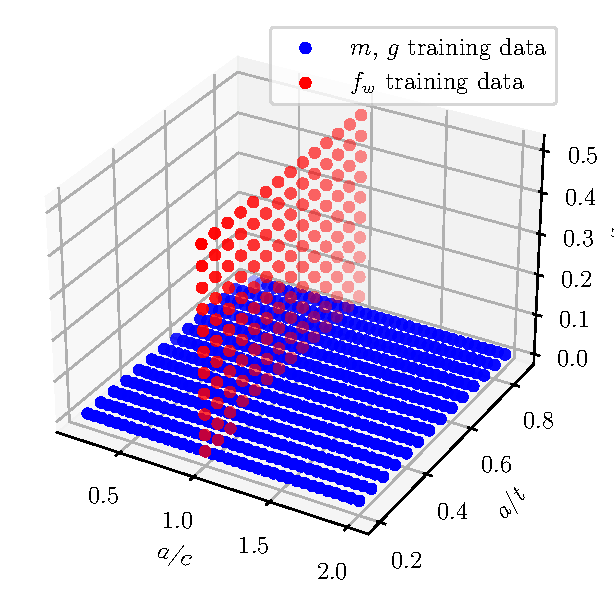
\includegraphics[width=\textwidth]{Figures_pdf/training_slices.pdf}
    \label{fig:training_models_3d}
    \caption{Visualization of the training data reduction allowed by the mechanics based approach. Each point represents a model in the training data-set. $f_w$ was trained when $\phi = \pi/2 \text{ and } a/c = 1$, $M$ was trained when $\phi=\pi/2 \text{ and } c/b = 0$, and $g$ was trained when $c/b = 0$ }
\end{figure}


During the training process, two techniques were employed to enhance the predictive ability and interpretability of the models. The first of these techniques involved the use of custom fitness functions to enforce the known constraints of each equation. These fitness functions assess the suitability of each candidate equation at the end of each training generation. The use of custom fitness functions ensures that all equations identified by the bingo algorithm adhere to the known limits of each equation, thereby improving interpretability. For instance, in equation \ref{eqn:fw_parameter_def}, as the values of $a/t$ and $c/b$ approach zero, the value of $f_w$ converges to 1. A fitness function that calculates the loss when this condition is met and assigns an infinite loss when it is not met enforces the equation's limits. Similar limit constraints apply to $M$ and $g$, such as $M(a/c = 1) = 1$ and $g(\phi = \pi/2) = 1$. The other method used to modify the training process was the addition of seed functions in the initial population. In the initial generation of the Bingo algorithm, a population of randomly generated equations is created. Using seeded equations allows the user to designate a fraction of these randomly generated equations as pre-set equations. This enables users to provide guidance to the algorithm. For example, upon visual examination of the training data for $g$, it was observed that $\left(1 - \sin\phi\right)^{a/t}$ appeared to fit the data well. Additional Bingo models were trained with this function seeded into the initial population. Other Bingo models were trained with only $1 - \sin\phi$ while other had no seeding at all. 


Training Bingo on the functions $f_w$ and $M$ was relatively fast only requiring 1-2 days due to the small training data-set, which only contained one data point per model when $\phi = \pi/2$. Additionally, these functions only required the discovery of relationships between two variables, namely, $c/b$ and $a/t$ for $f_w$, and $a/c$ and $a/t$ for $M$. However, training the function $g$ presented a different challenge due to the substantial increase in the number of data points as this function is now trained on every value of $\phi$ in each model. The Bingo algorithm tends to slow down as more data points are added. This results in a data-set comprising 300-400 data points per model, in contrast to the single data point per model for $f_w$ and $M$. To expedite the training of the $g$ function, two strategies were employed. The first involved down-sampling the $\phi$ data to reduce it to only 20 data points per model. The second strategy made use of a Bingo feature called the fitness predictor island (FPI). FPI aims to identify the optimal subset of the data that best represents the entire data-set. The size of this subset is determined by a hyper-parameter that specifies the fraction the subset. Even with theses two methods of reducing the number of data-points Bingo still took 5-7 days to train the $g$ models that did not contain $c/b$ and up to 13 days for the models that did contain $c/b$.


Once each training data-set has been computed bingo can be trained to find all three equations for $f_w$, $M$, and $g$ simultaneously. Multiple models were trained for each of the functions, due to the randomness of genetic programming this gave new equations that could be compared to one another to find the best combinations of $f_w$, $M$, and $g$ that predict SIF. The training process is done by first taking the SIF data computed from the FE model and then extracting the $f_w$, $M$, and $g$ training data-sets. Then bingo equations can be found for all three equations, these equation are then combined with the embedded ellipse solution from equation \ref{eqn:K_semi_with_l} to create a prediction for SIFS, this process is visualized in figure \ref{fig:training_flow}.

\begin{figure}
    \centering
    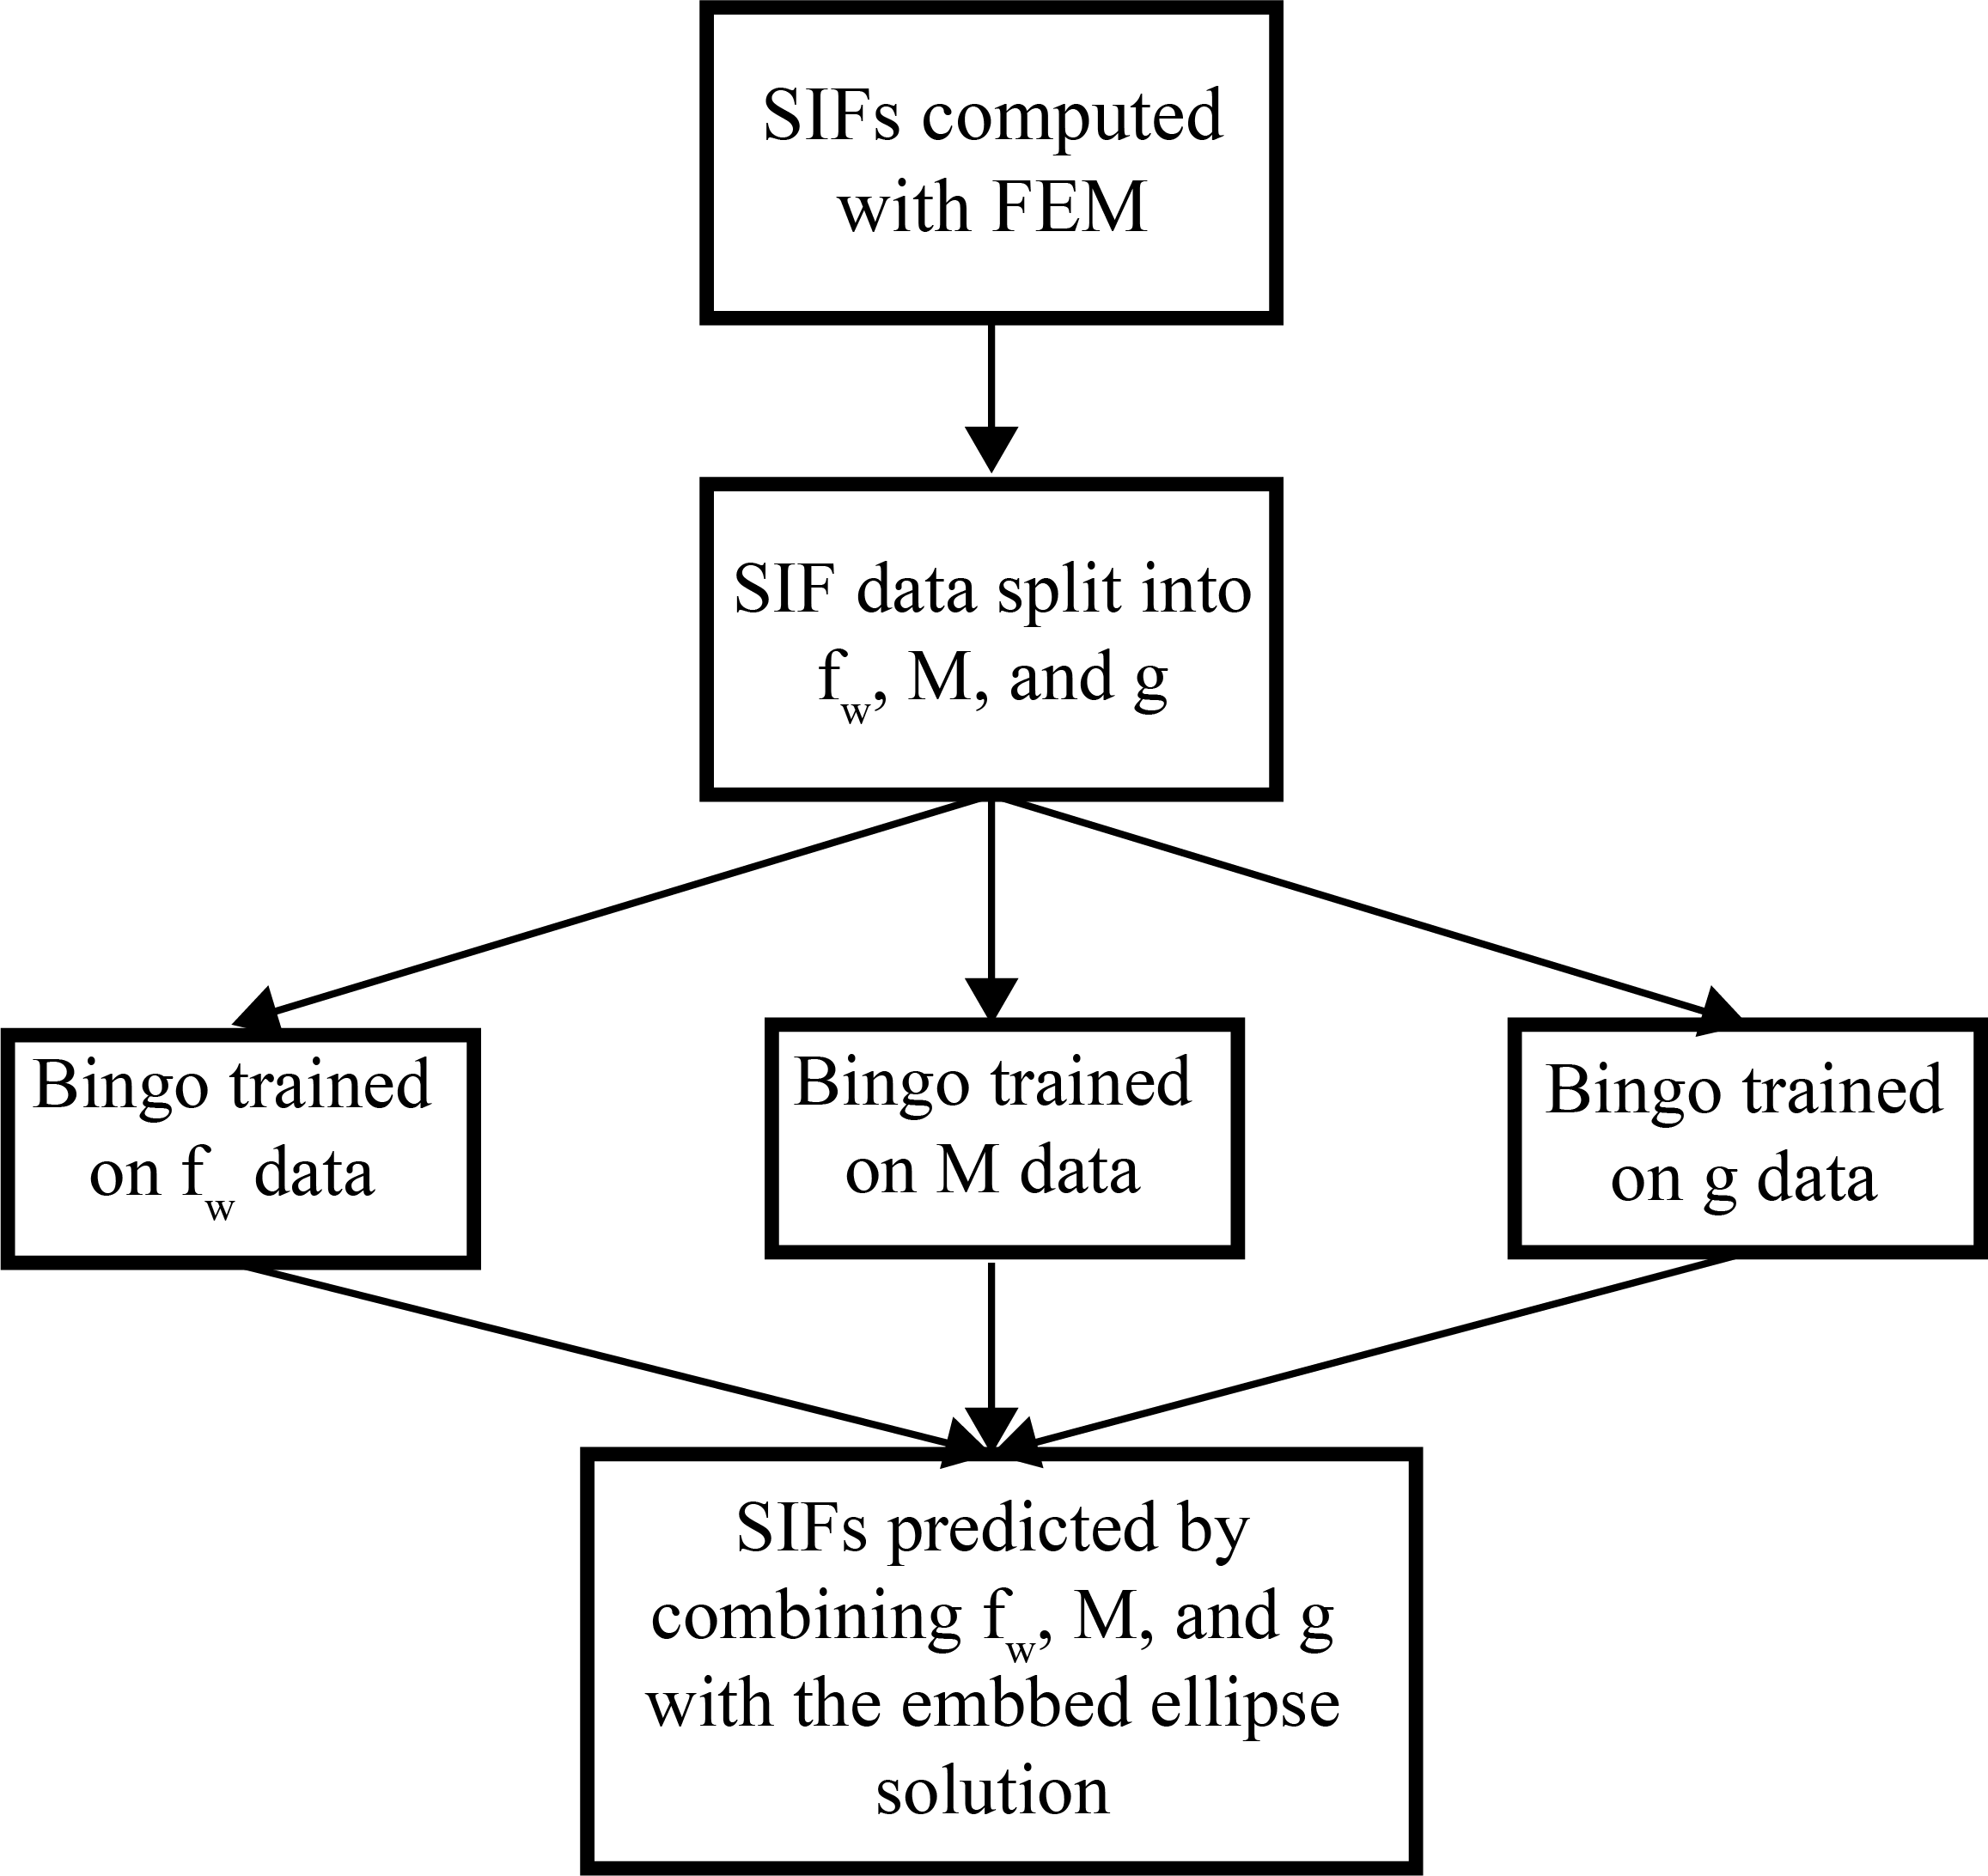
\includegraphics[width=\textwidth]{geometry_figures/training_flow.png}
    \label{fig:training_flow}
    \caption{Flow chart illustrating the training process of the three sub-functions $f_w$, $M$, and $g$}
\end{figure}





\section{Results}

After Bingo has been trained, it groups the best-performing equations into a Pareto front. In this graphical representation, the x-axis represents the complexity of each equation, while the y-axis signifies the fitness of each equation. Typically, models with lower complexity are more interpretable, but they may exhibit higher errors due to under-fitting. The Pareto front helps identify models that strike a balance between fitness and complexity.

The final SIF model can be selected in two ways. The first method involves selecting the equations for $f_w$, $M$, and $g$ individually and then combining them into a single SIF model. The alternative approach is to calculate all possible combinations of the candidate $f_w$, $M$, and $g$ equations to create a new Pareto front for the SIF models. This newly formed Pareto front is then used to choose the final model. Both of these methods aim to minimize complexity while ensuring fitness is at least as good as the equations from \cite{RNeqnsbook}.


Multiple equations were chosen for both of the model selection methods. This was done to create multiple comparison points between GPSR and the Raju-Newman equations. To lower the number of equations presented for the individual selection process the same $f_w$ (eqn \ref{eqn:Bingo_fw_common} and $M$ (eqn \ref{eqn:Bingo_M_common}) equations are used for all four models with only the $g$ equation changing.  

\begin{equation} \label{eqn:Bingo_fw_common}
    f_w = \sqrt{\frac{\sqrt{\frac{a}{t} + \cos\left(\frac{a}{t}\right)}}{\cos\left(\frac{c}{b}\right)}}
\end{equation}

\begin{equation} \label{eqn:Bingo_M_common}
    M = 1 + 0.06\left(\frac{a}{t}\right)^2\left(\frac{a}{c} - 1 \right) + \left(1 - \frac{c}{a} \right) \left(0.0069 \frac{c}{a} - 0.28 \frac{a}{t} \right)
\end{equation}


Using equation \ref{eqn:Bingo_g_matching_error} for $g$ creates a model for $K$ that has similar error to the Raju-Newman equation. Equation \ref{eqn:Bingo_g_matching_complexity} results in an a model with the same overall complexity as the Raju-Newman equation. 
The first model uses the data where $g$ was trained at $\frac{c}{b} = 0$ and 

Many Bingo runs were done with different parameters. The candidate equations can be selected from the combined Pareto front of all the bingo runs. 

Bingo equations are selected to compare with the Raju-Newman equations. First by matching the complexity of the equation and second by matching the error of the equations

the equations $f_w$ and $M$ have a smaller effect on the value of $KI$ than $g$, thus for consistency the same equations for $f_w$ and $M$ will be used for multiple models. Equation \ref{eqn:Bingo_g_matching_error} is the $g$ equation that produces a model with comparable error to the Raju-Newman equation. Equation \ref{eqn:Bingo_g_matching_complexity} results in a model with the same complexity as the Raju-Newman equation. Equation \ref{eqn:Bingo_g_matching_complexity_with_cb} also matches the overall complexity; however, the $g$ model was allowed to be trained on $c/b$. Equation \ref{eqn:Bingo_g_balance} has a balance of error and complexity. 

\begin{equation} \label{eqn:Bingo_g_matching_error}
    g = 1 + \frac{a}{t} \frac{1 - \sqrt{\sin \left( \phi \right)}}{\frac{a}{c} + 1}
\end{equation}

\begin{equation} \label{eqn:Bingo_g_matching_complexity}
\begin{gathered}
   g = 1 + 0.0316 \frac{a}{c} \left( \left( \sin\left(\phi\right) - 0.53 \right) \left( \left( \frac{a}{c} \right) ^ 1.54 - 1.18 \frac{a}{t} + 1.35 \right) - 2.6 \right) \left( \sin ^{\frac{a}{t} + 0.175}\left(\phi\right) - 1 \right) \\
   \frac{0.53 \left( \frac{a}{c} \right) ^ 1.54 - 0.625 \frac{a}{t} + 3.32}{\left( 0.739 \left( \frac{a}{c} \right) ^ 1.54 - 0.87 \frac{a}{t} + 1 \right) ^ 2} 
\end{gathered}
\end{equation}

\begin{equation} \label{eqn:Bingo_g_matching_complexity_with_cb}
    g = 1 + \frac{{\left({0.78}{\left({0.66}-{1.37} \sin{{\left({0.32}\frac{a}{{c}}\frac{a}{{t}}{\left(\frac{a}{{t}}-\frac{c}{{b}}\right)}-\frac{a}{{t}}+{1.76}\right)}}\right)}{\left( \sin{{\left(\phi\right)}}+{6.1}\right)}+{4.02}\right)}{\left( \sin{{\left(\phi\right)}}-{1}\right)}}{{{\left({0.656}-{1.37} \sin{{\left({0.32}\frac{a}{{c}}\frac{a}{{t}}{\left(\frac{a}{{t}}-\frac{c}{{b}}\right)}-\frac{a}{{t}}+{1.76}\right)}}\right)}{\left( \sin{{\left(\phi\right)}}+{6.1}\right)}}}
\end{equation}

\begin{equation} \label{eqn:Bingo_g_balance}
    g = 1 + \frac{0.4 \frac{a}{c}\left(1 - \sin\left(\phi\right) ^ \frac{a}{t} \right)}{\left( \frac{a}{c} \right) ^ 2 - \frac{a}{t} + 1}
\end{equation}

Figure \ref{fig:perato_front} shows the Pareto fronts for all 3 equations. The distributions of the errors for each of the four models along with with Raju-Newman equation are shown in figure \ref{fig:error_plots}. The parity plots for each model is also shown in figure \ref{fig:error_plots}.
\begin{figure}%
    \centering
    \subfloat[\centering Distributions of error]{{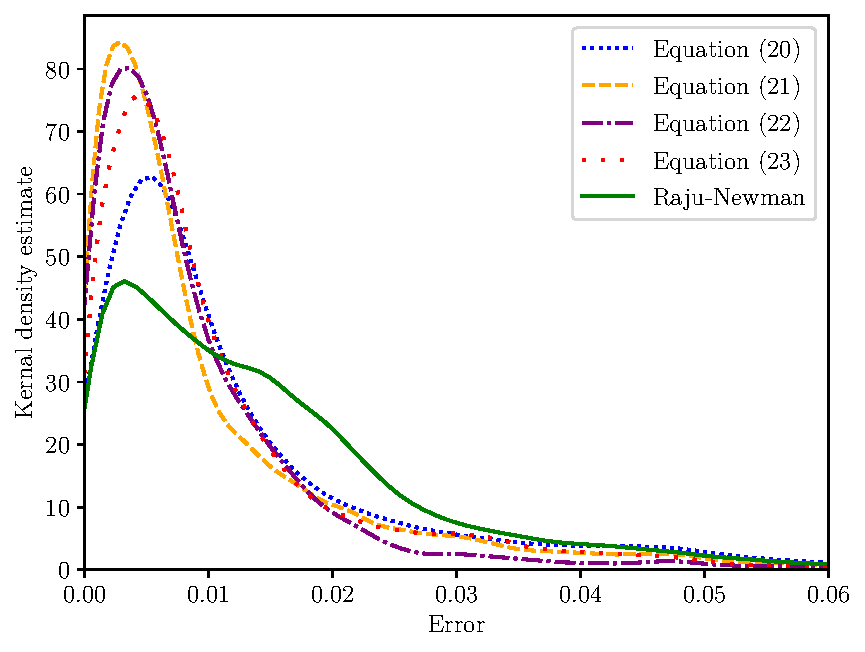
\includegraphics[width=0.45\textwidth]{Figures_pdf/kde.pdf} }}%
    \qquad
    \subfloat[\centering Parity plots]{{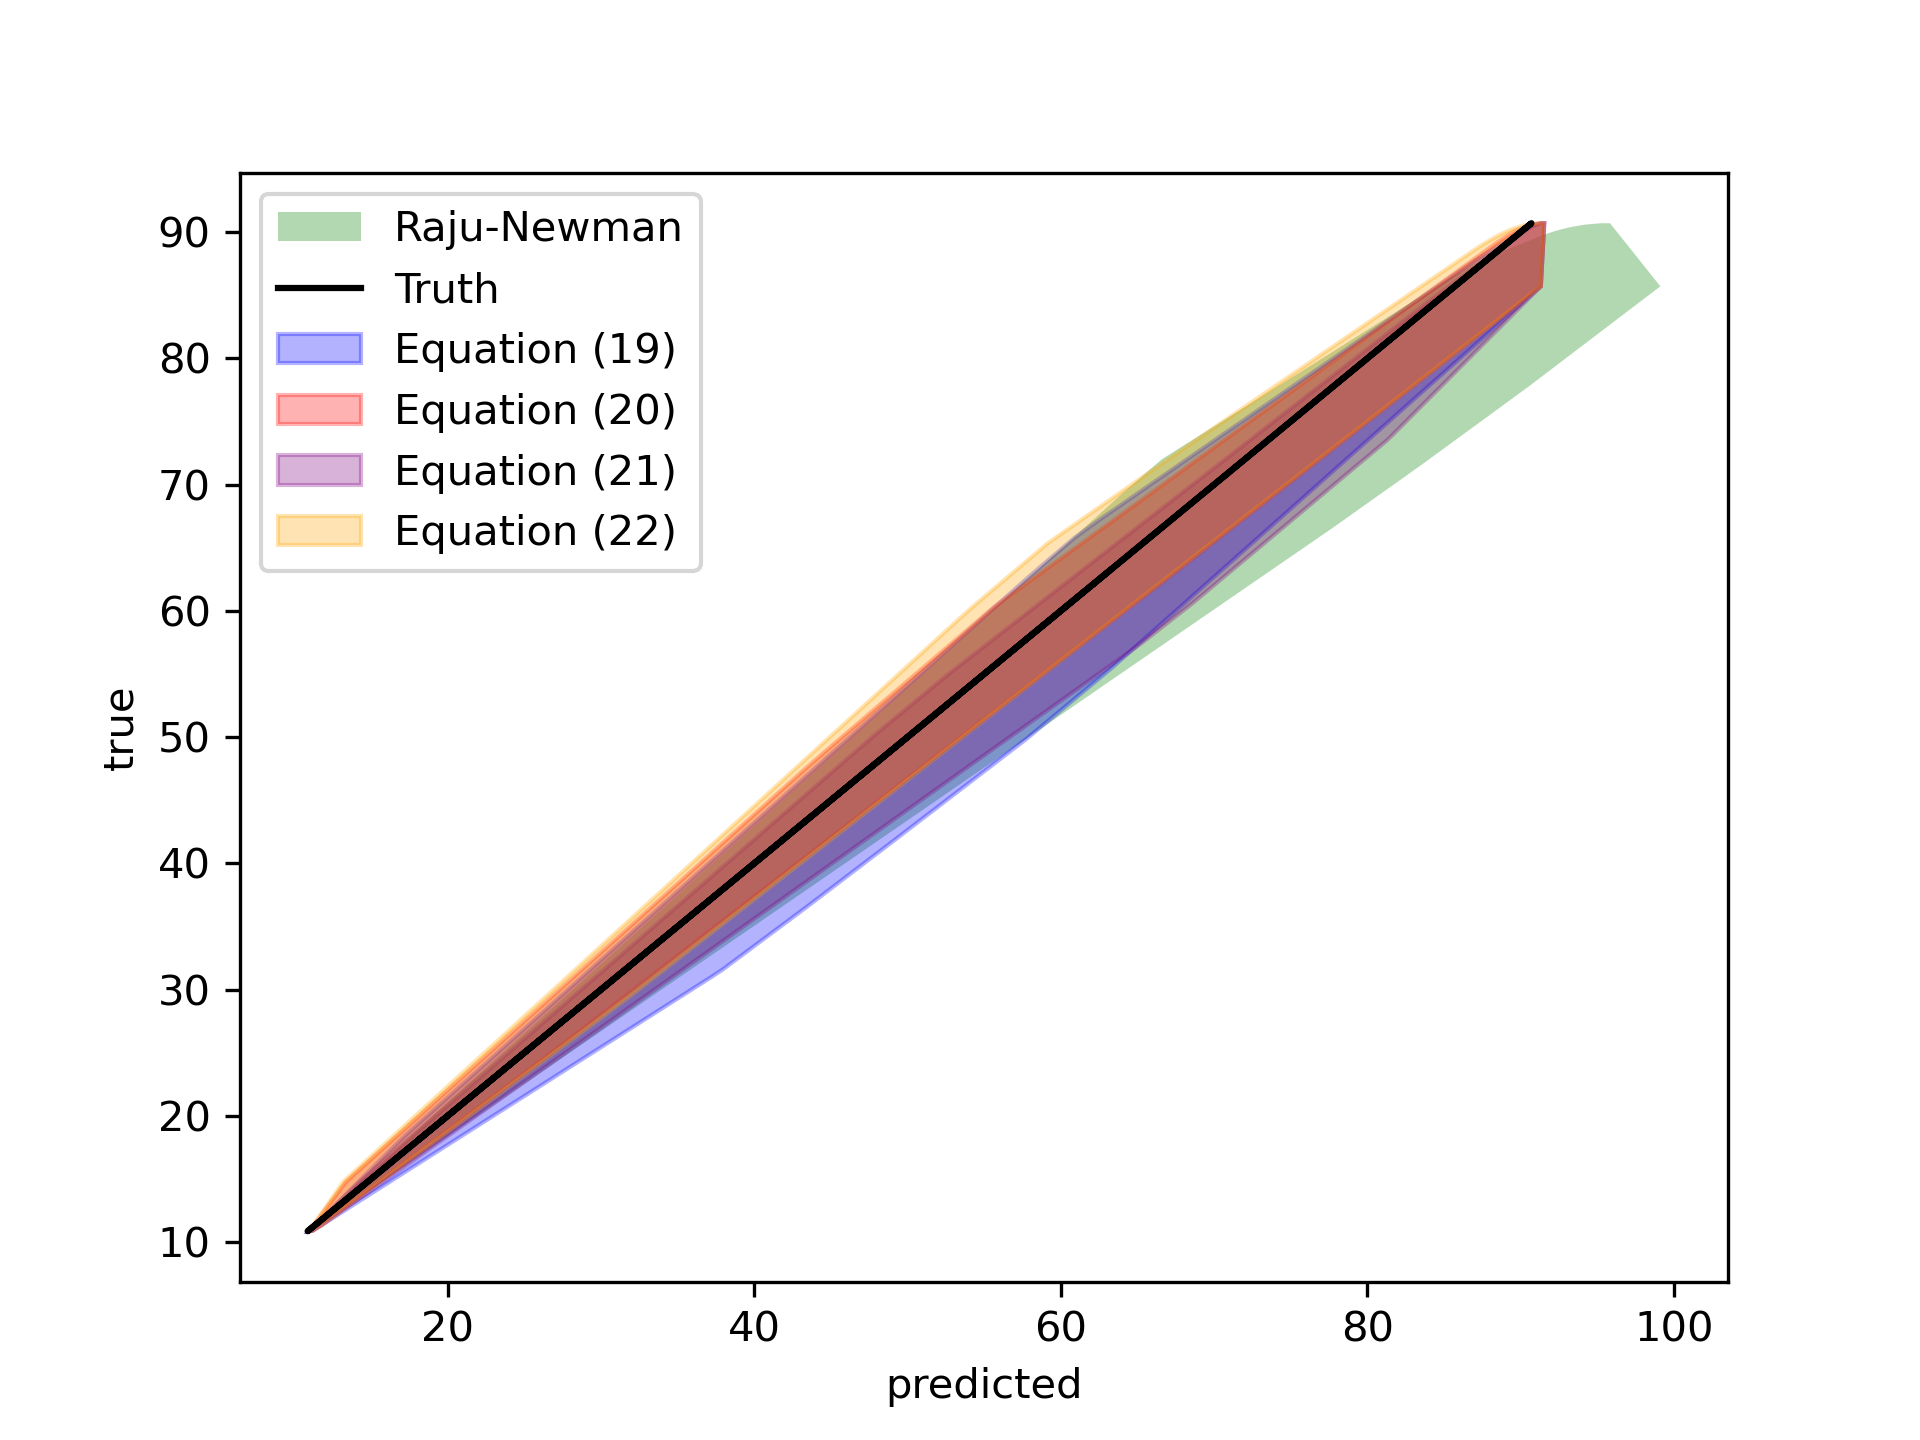
\includegraphics[width=0.45\textwidth]{Figures/parity_plot.png} }}%
    \caption{(a) Density plot for the errors of each of the equations. (b) Parity plot with each of the different equations.}%
    \label{fig:error_plots}%
\end{figure}

\begin{figure}
    \centering
    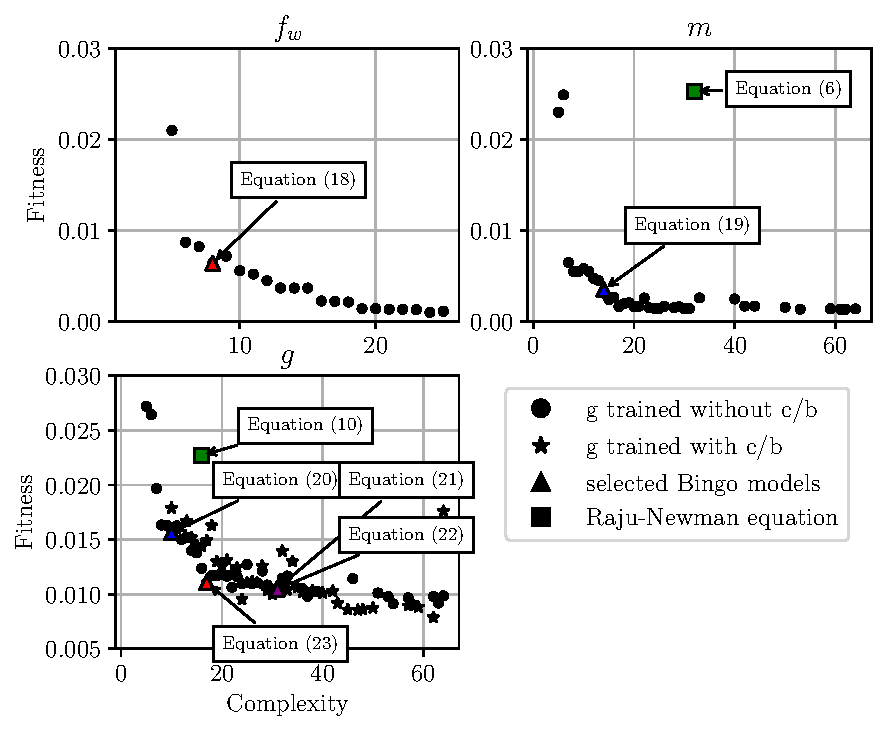
\includegraphics[width=\textwidth]{Figures_pdf/Pareto_fronts.pdf}
    \label{fig:perato_front}
    \caption{Pareto fronts for $f_w$, $M$, and $g$. $f_w$ and $M$ have the same equation for all four models. Both the Pareto fronts for $g$ with and without $c/b$ are shown} 
\end{figure}

\begin{figure}%
    \centering
    \subfloat[\centering Distributions of error]{{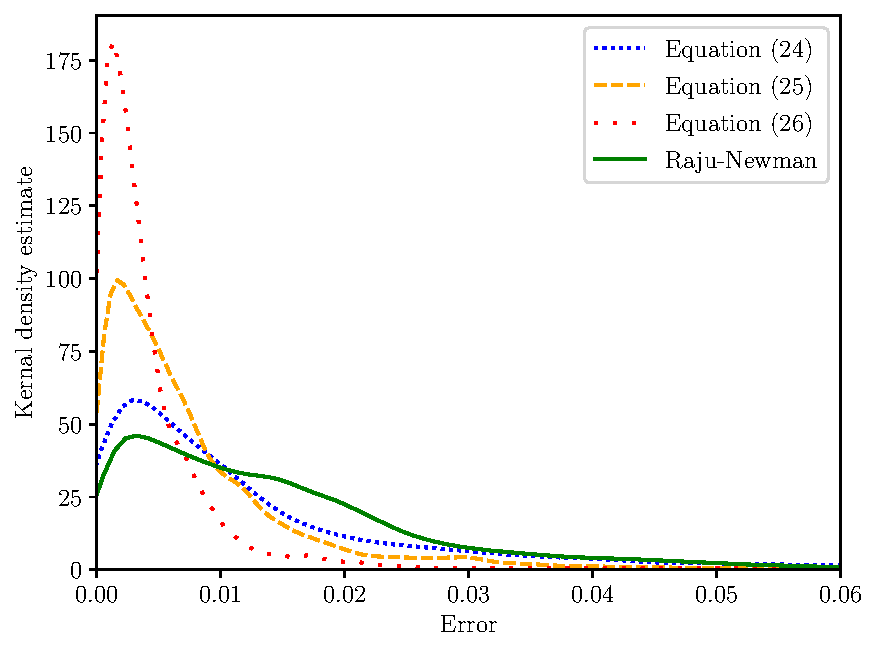
\includegraphics[width=0.45\textwidth]{Figures_pdf/kde_combo.pdf} }}%
    \qquad
    \subfloat[\centering Parity plots]{{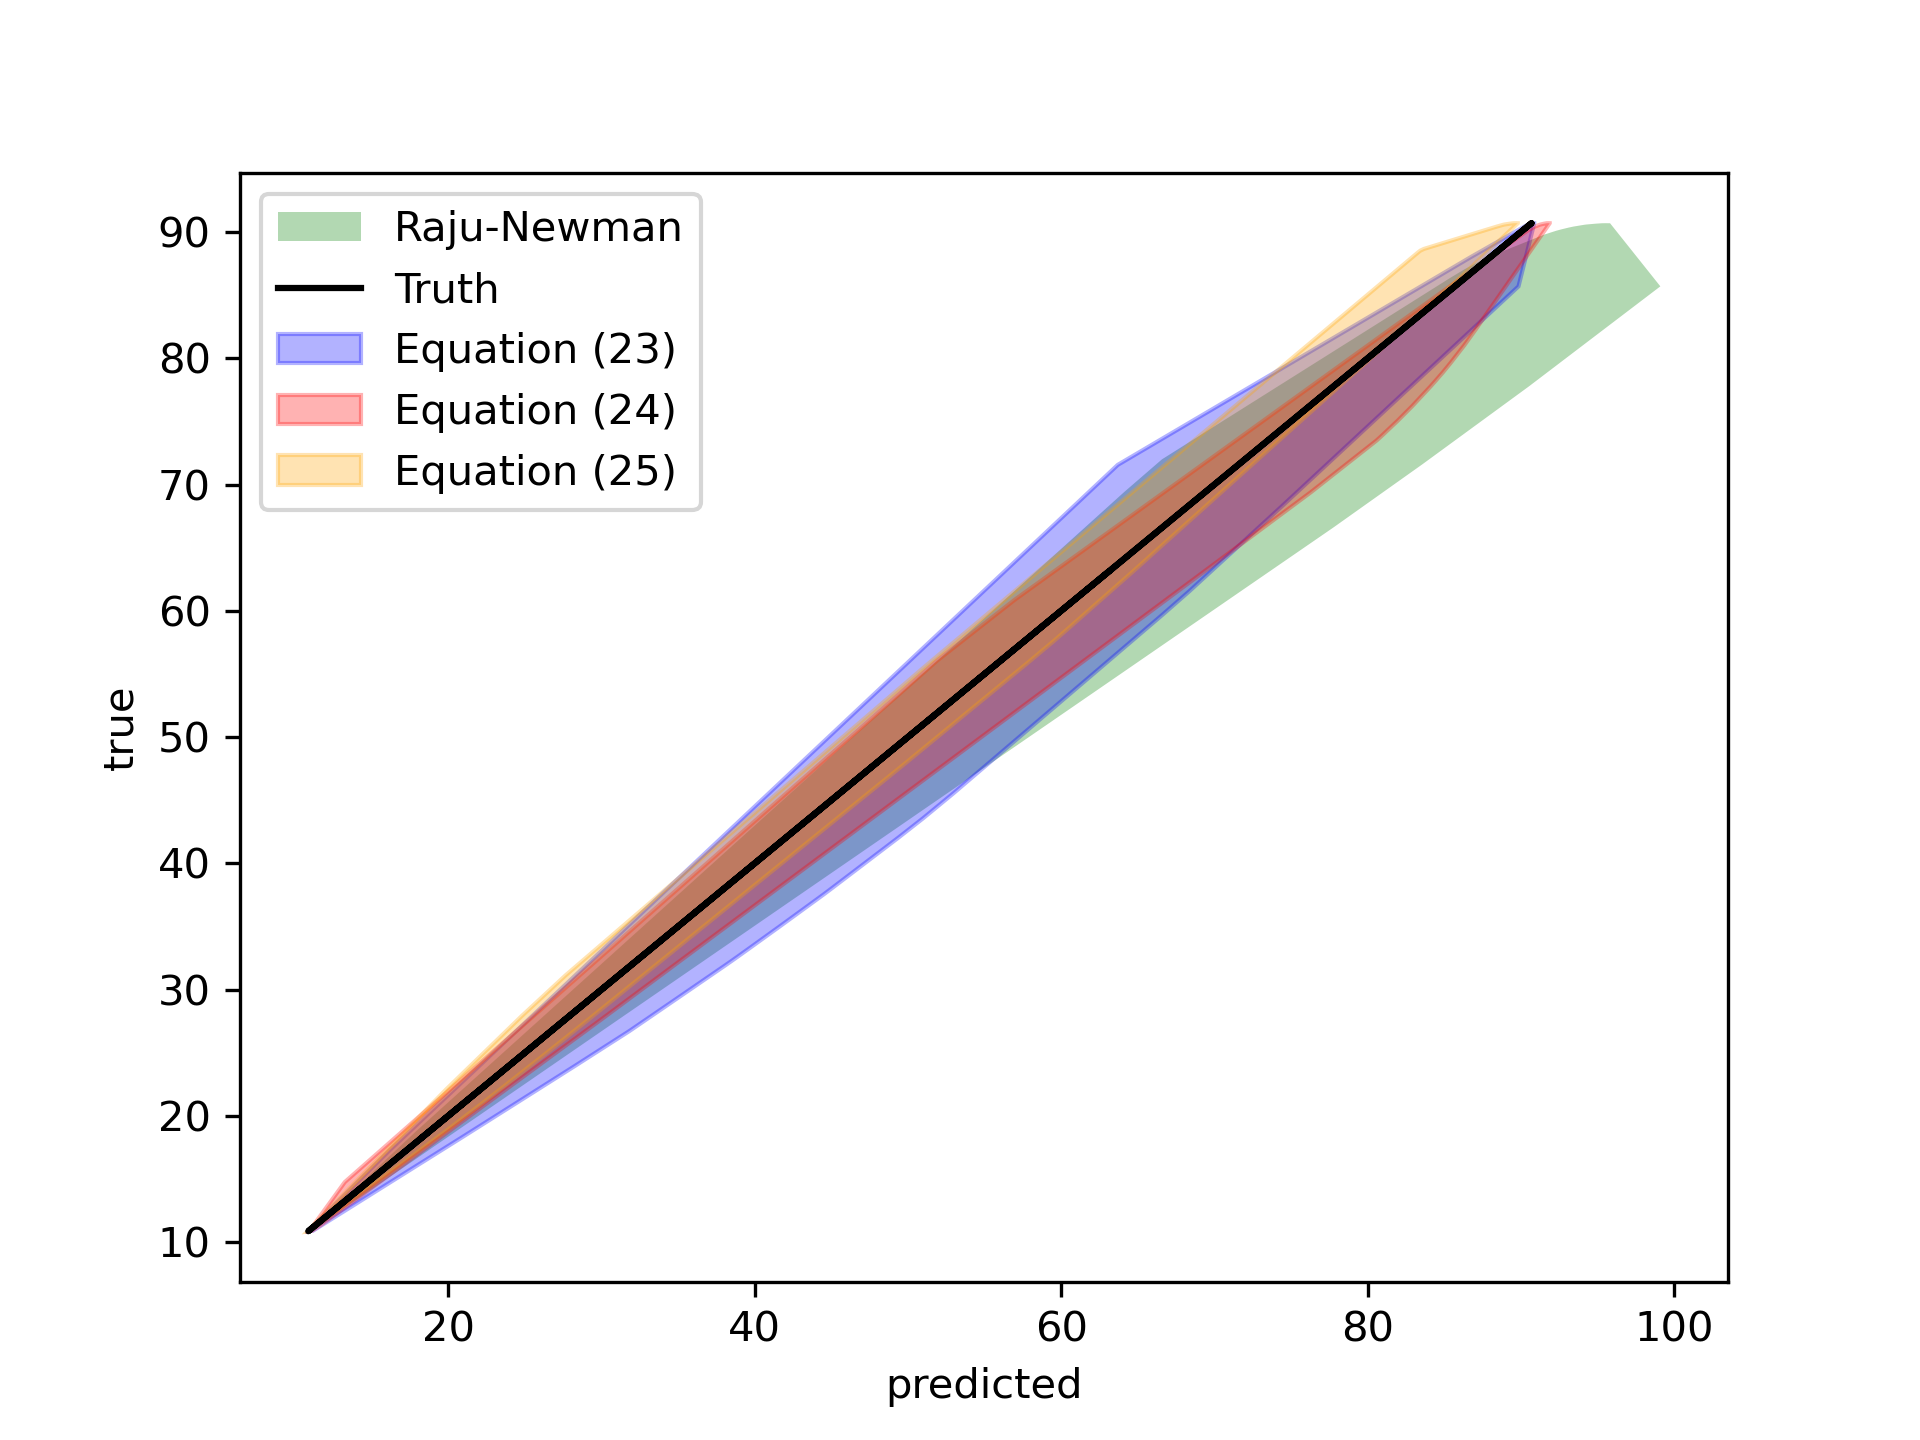
\includegraphics[width=0.45\textwidth]{Figures/parity_plot_everything.png} }}%
    \caption{(a) Density plot for the errors of each of the equations from the combined selection. (b) Parity plot with each of the different equations from the combined selection.}%
    \label{fig:combo_error_plots}%
\end{figure}


The Pareto front for the model selection using the Pareto front generated using all possible combinations of the models $f_w$, $M$, and $g$ can be seen in figure \ref{fig:perato_front_everything}. Equations [\ref{eqn:Bingo_matching_error_combo}-\ref{eqn:Bingo_optimal_combo}] are the equations gathered from the Pareto front of all possible equations. The error distributions and parity plots for these models can be seen in figure \ref{fig:combo_error_plots}.

\begin{equation} \label{eqn:Bingo_matching_error_combo}
    \begin{cases}
        f_w = 0.13 \frac{c}{b} + 0.13 \frac{a}{t} + 1.0
        \\
        M = - 0.223 \frac{a}{t} + 1 + \frac{0.223 \frac{a}{t}}{\frac{a}{c}}
        \\
        g = 0.554 \frac{a}{t} \left(1 - \sin^{0.491^{\frac{a}{c}}}{\left(\phi \right)}\right)
    \end{cases}
\end{equation}

\begin{equation} \label{eqn:Bingo_matching_complexity_combo}
    \begin{cases}
        f_w = \frac{- 63.94 \frac{c}{b} + 51.875 \frac{a}{t} + 38.855}{- 63.94 \frac{c}{b} + 43.336 \frac{a}{t} + 38.855}
        \\
        M = \frac{- 0.028 \frac{a}{c}^{3} + \frac{a}{c}^{2} \left(\frac{a}{c} + 0.028\right) - 0.644 \frac{a}{c} \frac{a}{t} \left(\frac{a}{c} \frac{a}{t} - 0.044\right) \left(- \frac{a}{c} \left(\frac{a}{t} - 1.103\right) + 0.044\right) + 0.644 \frac{a}{t} \left(\frac{a}{c} \frac{a}{t} - 0.044\right) \left(- \frac{a}{c} \left(\frac{a}{t} - 1.103\right) + 0.044\right)}{\frac{a}{c}^{3}}
        \\
        g = - \frac{0.127 \frac{a}{c} \left(\sin^{\frac{a}{t}}{\left(\phi \right)} - 1\right)}{\left(\cos{\left(\frac{c}{b} \right)} - 0.66\right) \left(\frac{a}{c}^{1.811} - 1.066 \frac{a}{t} + 0.992\right)}
    \end{cases}
\end{equation}

\begin{equation} \label{eqn:Bingo_optimal_combo}
    \begin{cases}
        f_w = - \frac{a}{t} \left(\left(1.216 \frac{c}{b}^{2} + 0.11\right) \left(\frac{a}{t} - \sqrt{- \frac{c}{b}^{2} - 0.751}\right) - 0.119\right) + 1.0
        \\
        M = \frac{a}{c}^{\frac{- 0.037 \frac{a}{c} - 0.046 \frac{a}{t} \left(\frac{a}{c}^{2} - 15.413\right) \left(\frac{a}{t} - 1.114\right) \left(1.919 \frac{a}{t} - 0.489\right) - 0.06}{\frac{a}{c} + 0.599}}
        \\
        g = - \frac{1.232 \left(\frac{a}{c} \left(\frac{a}{c} + 0.06\right) \left(0.103 \left(1 - \sin{\left(\phi \right)}\right)^{\frac{3}{2}} + 0.017\right) - 0.36 \left(\frac{a}{t} - 0.187\right) \left(\frac{a}{c} \left(\left(\frac{a}{c} + 0.06\right) \left(0.017 \frac{a}{c} + 0.033 \frac{a}{t} - 0.409 \frac{c}{b}^{2} \right) - 0.646\right) \left(\frac{a}{c} + 2 \frac{a}{t} \right) + 2.501 \frac{a}{c} + 0.1501\right)\right) \left(\sin{\left(\phi \right)} - 1\right)}{\frac{a}{c} \left(\frac{a}{c} + 0.06\right)}
    \end{cases}
\end{equation}


\begin{figure}
    \centering
    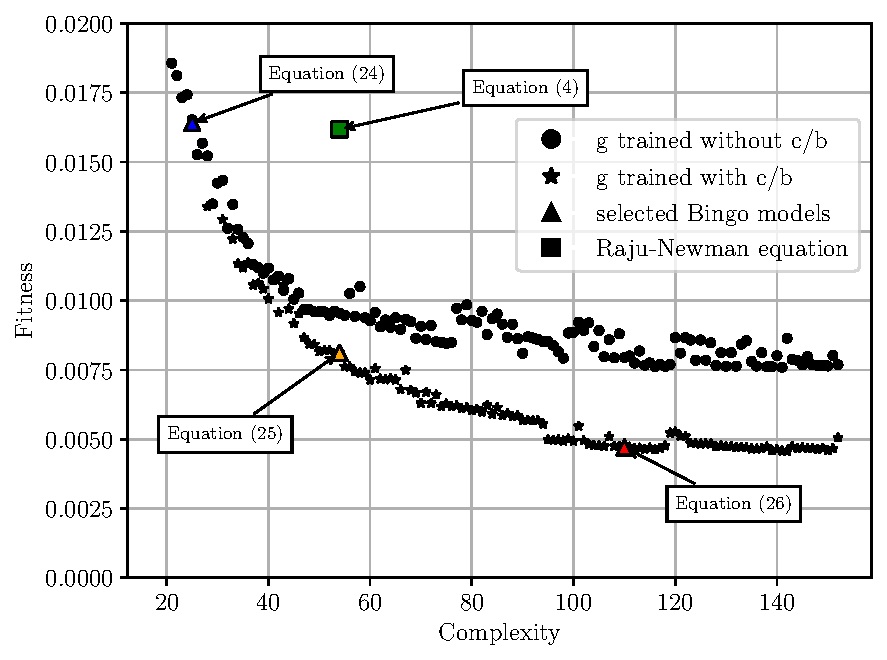
\includegraphics[width=\textwidth]{Figures_pdf/Pareto_fronts_combo.pdf}
    \label{fig:perato_front_everything}
    \caption{Pareto front for the models selected using all possible combinations.}
\end{figure}


Finally figure \ref{fig:perato_front_everything} shows all eight models on the same Pareto front. 

\begin{figure}
    \centering
    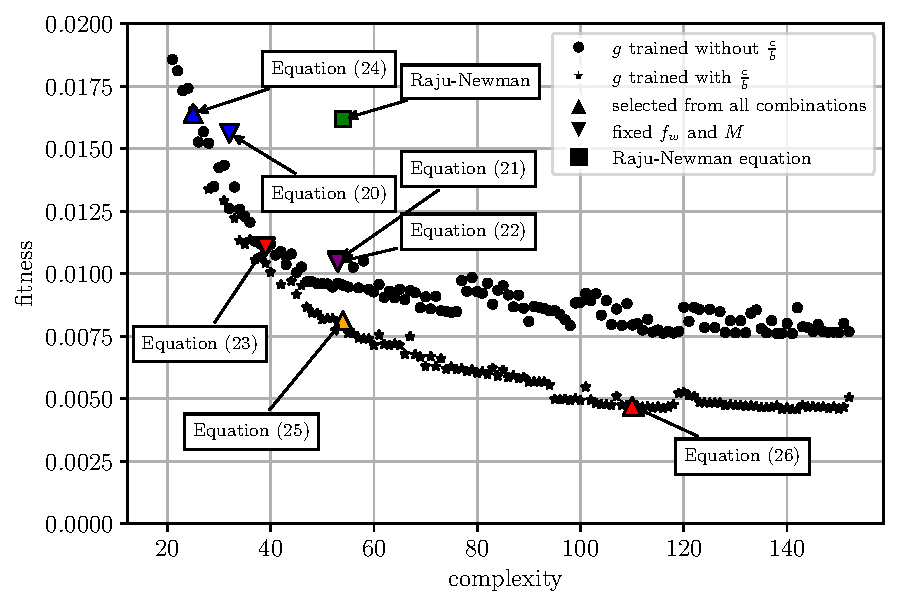
\includegraphics[width=\textwidth]{Figures_pdf/Pareto_fronts_everything.pdf}
    \label{fig:perato_front_everythin}
    \caption{Pareto front with all models the triangle markers correspond to the models that were individually selected and the square markers are the models selected using all possible combinations.}
\end{figure}

\begin{figure}
    \centering
    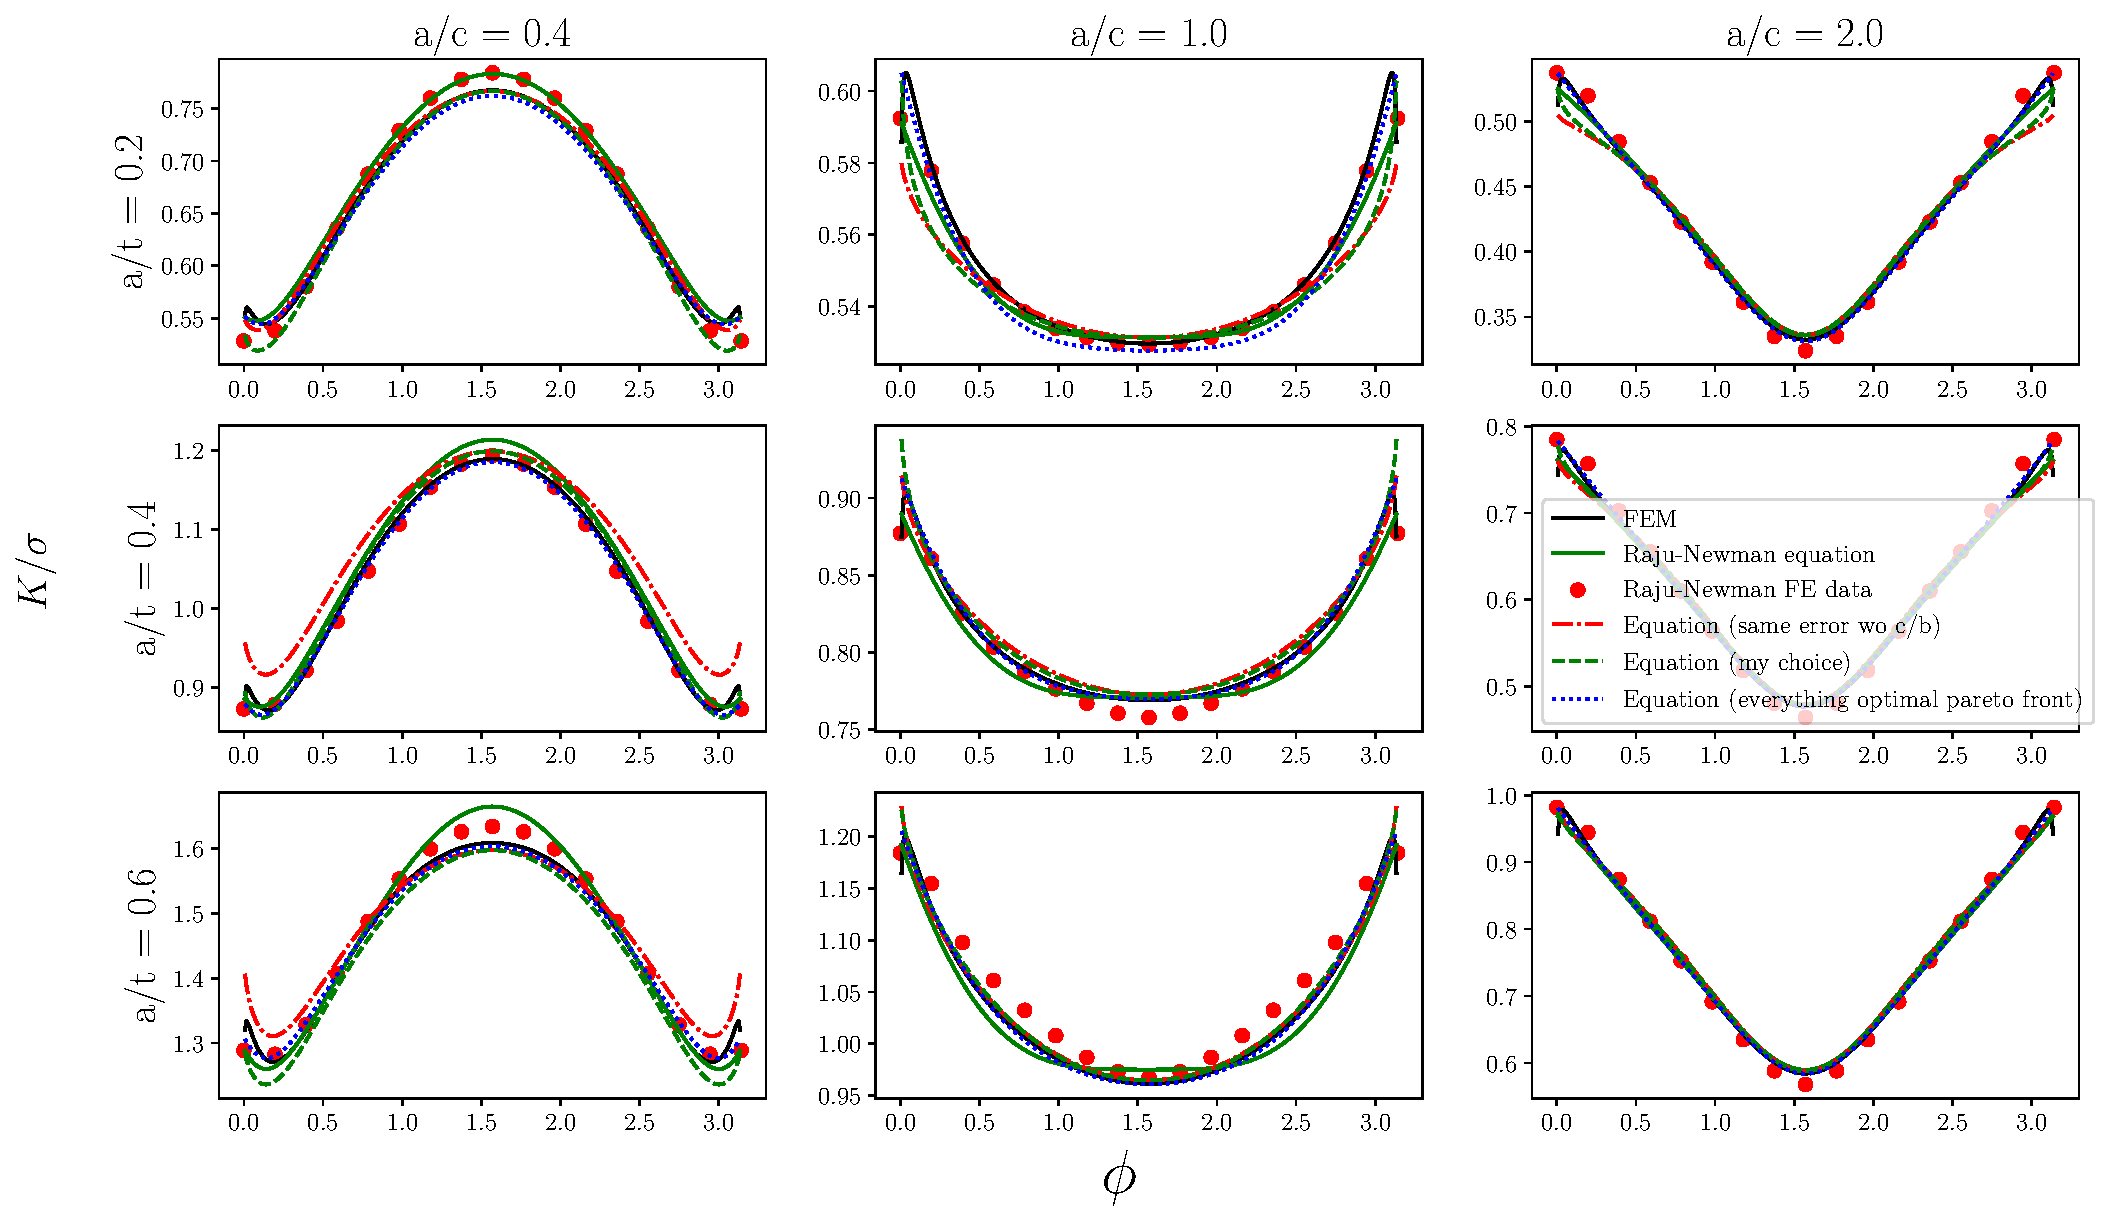
\includegraphics[width=\textwidth]{Figures_pdf/K_data_with_bingo.pdf}
    \label{fig:K_data_with_bingo}
    \caption{A sample of models comparing the SIFs collected from FRANC3D with the bingo equation, the Raju-Newman equation, and the Raju-Newman FE data.}
\end{figure}
\section{Discussion}
% Interpretetabiliyt vs error and how we approach the high accuracy models






GPSR offers the advantage of generating a population of equations, providing users with the flexibility to choose the equation that best suits their specific needs. Typically, the optimal equation strikes a balance between simplicity and accuracy. However, certain scenarios may necessitate either maximum accuracy or very simple equations. This study presents various models with varying levels of accuracy and complexity. The SIF equation was derived using two methods from the $f_w$, $m$, and $g$ equations. The first method involved using fixed $f_w$ and $m$ equations, as the $g$ equation has the most significant impact on overall SIF accuracy. The equations obtained through this method are illustrated in Figure \ref{fig:perato_front}. The second method employed every possible combination of the $f_w$, $m$, and $g$ equations generated by Bingo, with the extracted equations depicted in Figure \ref{fig:perato_front_everything}. To facilitate comparison with the Raju and Newman equation, models were selected based on similar errors and complexities, as shown in Figure \ref{fig:perato_front_everything_ant_more}. The comparison revealed that Bingo outperforms the Raju and Newman equation in both complexity and error. Models with similar complexity demonstrated lower errors, while models with similar errors exhibited considerably lower complexities.

When applying the same approach as Raju and Newman to decompose $K$ using $f_w$, $M$, and $g$, the influence of $c/b$ is not entirely captured. The finite width of the model is considered only in the function $f_w$, which is not dependent on $\phi$. Consequently, there is no coupling between $\phi$ and $c/b$. This is evident in Figure \ref{fig:perato_front_everything}, where models allowing $c/b$ in $g$ outperform those that do not, particularly beyond a complexity of approximately 40. This discrepancy is observed specifically in models derived from every combination of $f_w$, $M$, and $g$. However, in the case of fixed $f_w$ and $M$ functions, whether or not $c/b$ is utilized in $g$ does not seem to alter the results, as shown in Figure \ref{fig:perato_front}. This is attributed to the specific $f_w$ equation chosen not being influenced by $c/b$ in $g$. Neglecting the interaction between $\phi$ and $c/b$ allows for the rapid creation of simpler models, significantly reducing the number of FE models required for training. Nonetheless, if a highly accurate model is essential, employing the entire domain for training enables the attainment of higher accuracy.



\subsection{Model limitations}

It was observed that, across all trained Bingo models, the highest errors occurred at the crack surface where $\phi$ is close to $0$ or $\pi$ and when $a/c$ is at its smallest value of $0.2$. At the crack surface where $\phi = \pi, 0$, the SIF values exhibit a sharp decline due to the influence of plane stress vs. plane strain conditions. The Bingo model struggles to fully capture this region because of a lack of data at the surfaces. It might be possible to address these surface effects by introducing an additional correction factor that specifically accounts for the model's surfaces. The reason for the highest errors occurring at $a/c = 0.2$ is that this represents the lower bound of the training data, and there is also a significant change in the SIF data in this region. Without information about SIFs for values smaller than $a/c = 0.2$ in the training data, Bingo fits this region of the data less accurately. Including smaller aspect ratios in the training data could likely reduce the maximum error of the model. However, it's worth noting that $a/c = 0.2$ is already a relatively small aspect ratio, and the rest of the domain with aspect ratios above $a/c = 0.2$ have very low error.


\subsection{Comparison with Black Box methods}



Comparing the results shown here from Bingo with other ML methods such as the ones used in \cite{Tushar}. Figure \ref{fig:bingo_ml_comp} shows Bingo and the Raju-Newman equation compared with two commonly used ML methods for a data-set of this size, support vector machine regression (SVM) and random forest regression (RFR). Using the optimal hyper-parameters from \cite{Tushar} and training directly on $K$ results in the square markers on the plot. Training the models again using the mechanics bases approach used in this research, results in the circle points. From this figure, the error of the RFR is reduced by using the mechanics based approach, while the SVM produces worse error when using the mechanics based approach. One possible reason that the SVM produces a worse model when using the mechanics based approach, is that it cannot fit to the smaller data-sets, while Bingo and RFR are easily able to fit to fewer data-points. It is shown in \cite{tushar} that as the data-points decrease to 100 that SVM performs worse. Being able to produce accurate models with fewer data-points is a strength as having many training examples is rarely feasible. Comparing the evaluation times of each of the ML models shown in \ref{fig:bingo_ml_comp} shows that bingo and the Raju-Newman have similar evaluation times, however, the black box models are slower with the random forest taking 3 seconds to evaluate the data-set, and SVM taking 40 seconds. 
\begin{figure}
    \centering
    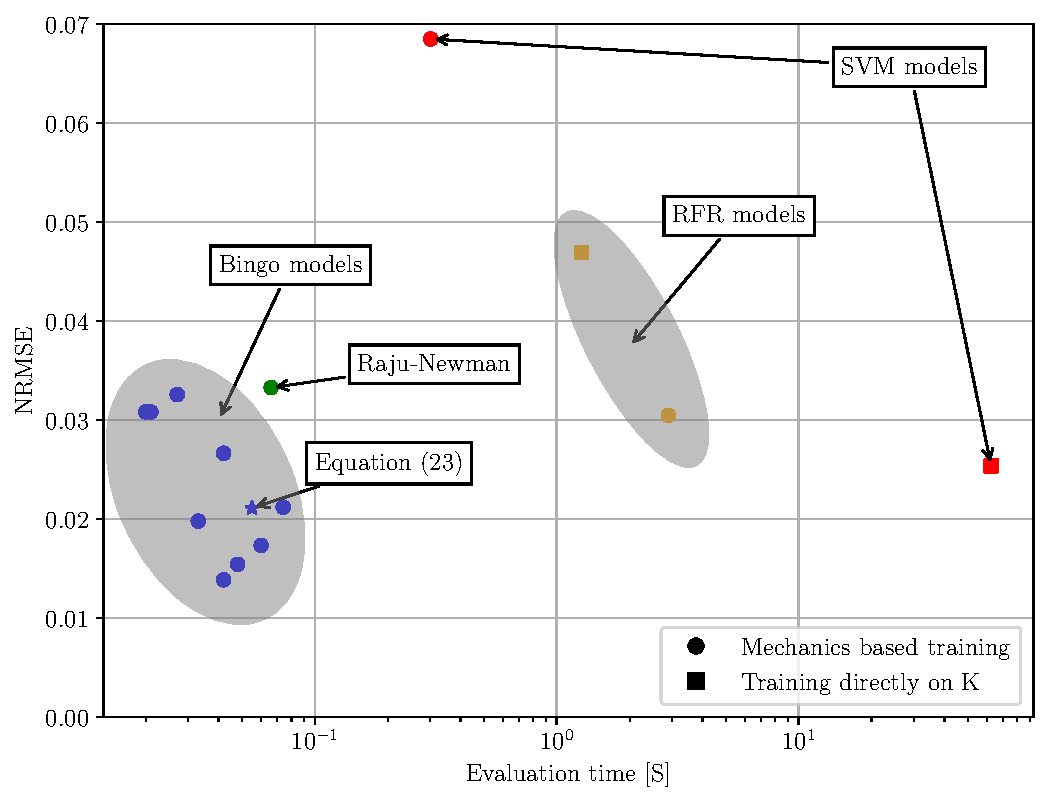
\includegraphics[width=\textwidth]{Figures_pdf/bingo_ml_comp.pdf}
    \label{fig:bingo_ml_comp}
    \caption{Plot comparing training times and errors between Bingo, Raju-Newman equation, RFR, and SVM. The circular markers were all trained using the mechanics based approach presented in this research, the square makers were trained directly on K. The evaluation times were measured on one core of an Intel i7-4790 with 32Gb DDR3 RAM at 1600 MHz on a data-set containing 150k data-points.}
\end{figure}
 

Bingo outperforms SVM and RFR both in evaluation time and error, while also producing an explainable closed form equation. Some of the Bingo models only needed a small subset of the data to be able to predict SIF for the entire domain. Bingo does, however, have a downside in its long training time on the order of hours to days, while SVM and RFR can be trained very quickly on the order of seconds to minutes. Bingo takes more effort than SVM and RFR to create a model for this data-set, however, the final model created by Bingo outperforms SVM, RFR, and the Raju-Newman equation in all metrics. 






\section{Conclusion}
By incorporating knowledge of fracture mechanics into the training process, GPSR is able to create models that can outperform traditional ML methods in both accuracy and explainability. The main limitation of GPSR is its expensive training process. This reduces the number of parameters that can be used making it more difficult to apply to more complex problems. By using the framework proposed here it is possible to create a library of SIF equations for many crack cases that currently have no handbook solutions.


\bibliographystyle{unsrt}
\bibliography{library.bib}
%\printbibliography
\newpage

%\begin{table}[]
\centering
\begin{tabular}{|l|l|l|}
\hline
\textbf{Feature} & \textbf{min} & \textbf{max} \\ \hline
a/c              & 0.2          & 2            \\ \hline
a/t              & 0.2          & 0.85          \\ \hline
c/b              & 0.01         & 0.5          \\ \hline
$\phi$           & 0            & $\pi$        \\ \hline
\end{tabular}
\caption{Max and min values for each of the features used when creating the cracked FE models}
\label{table_feat_range}
\end{table}

\begin{figure}%
    \centering
    \subfloat[\centering Applied boundary conditions]{{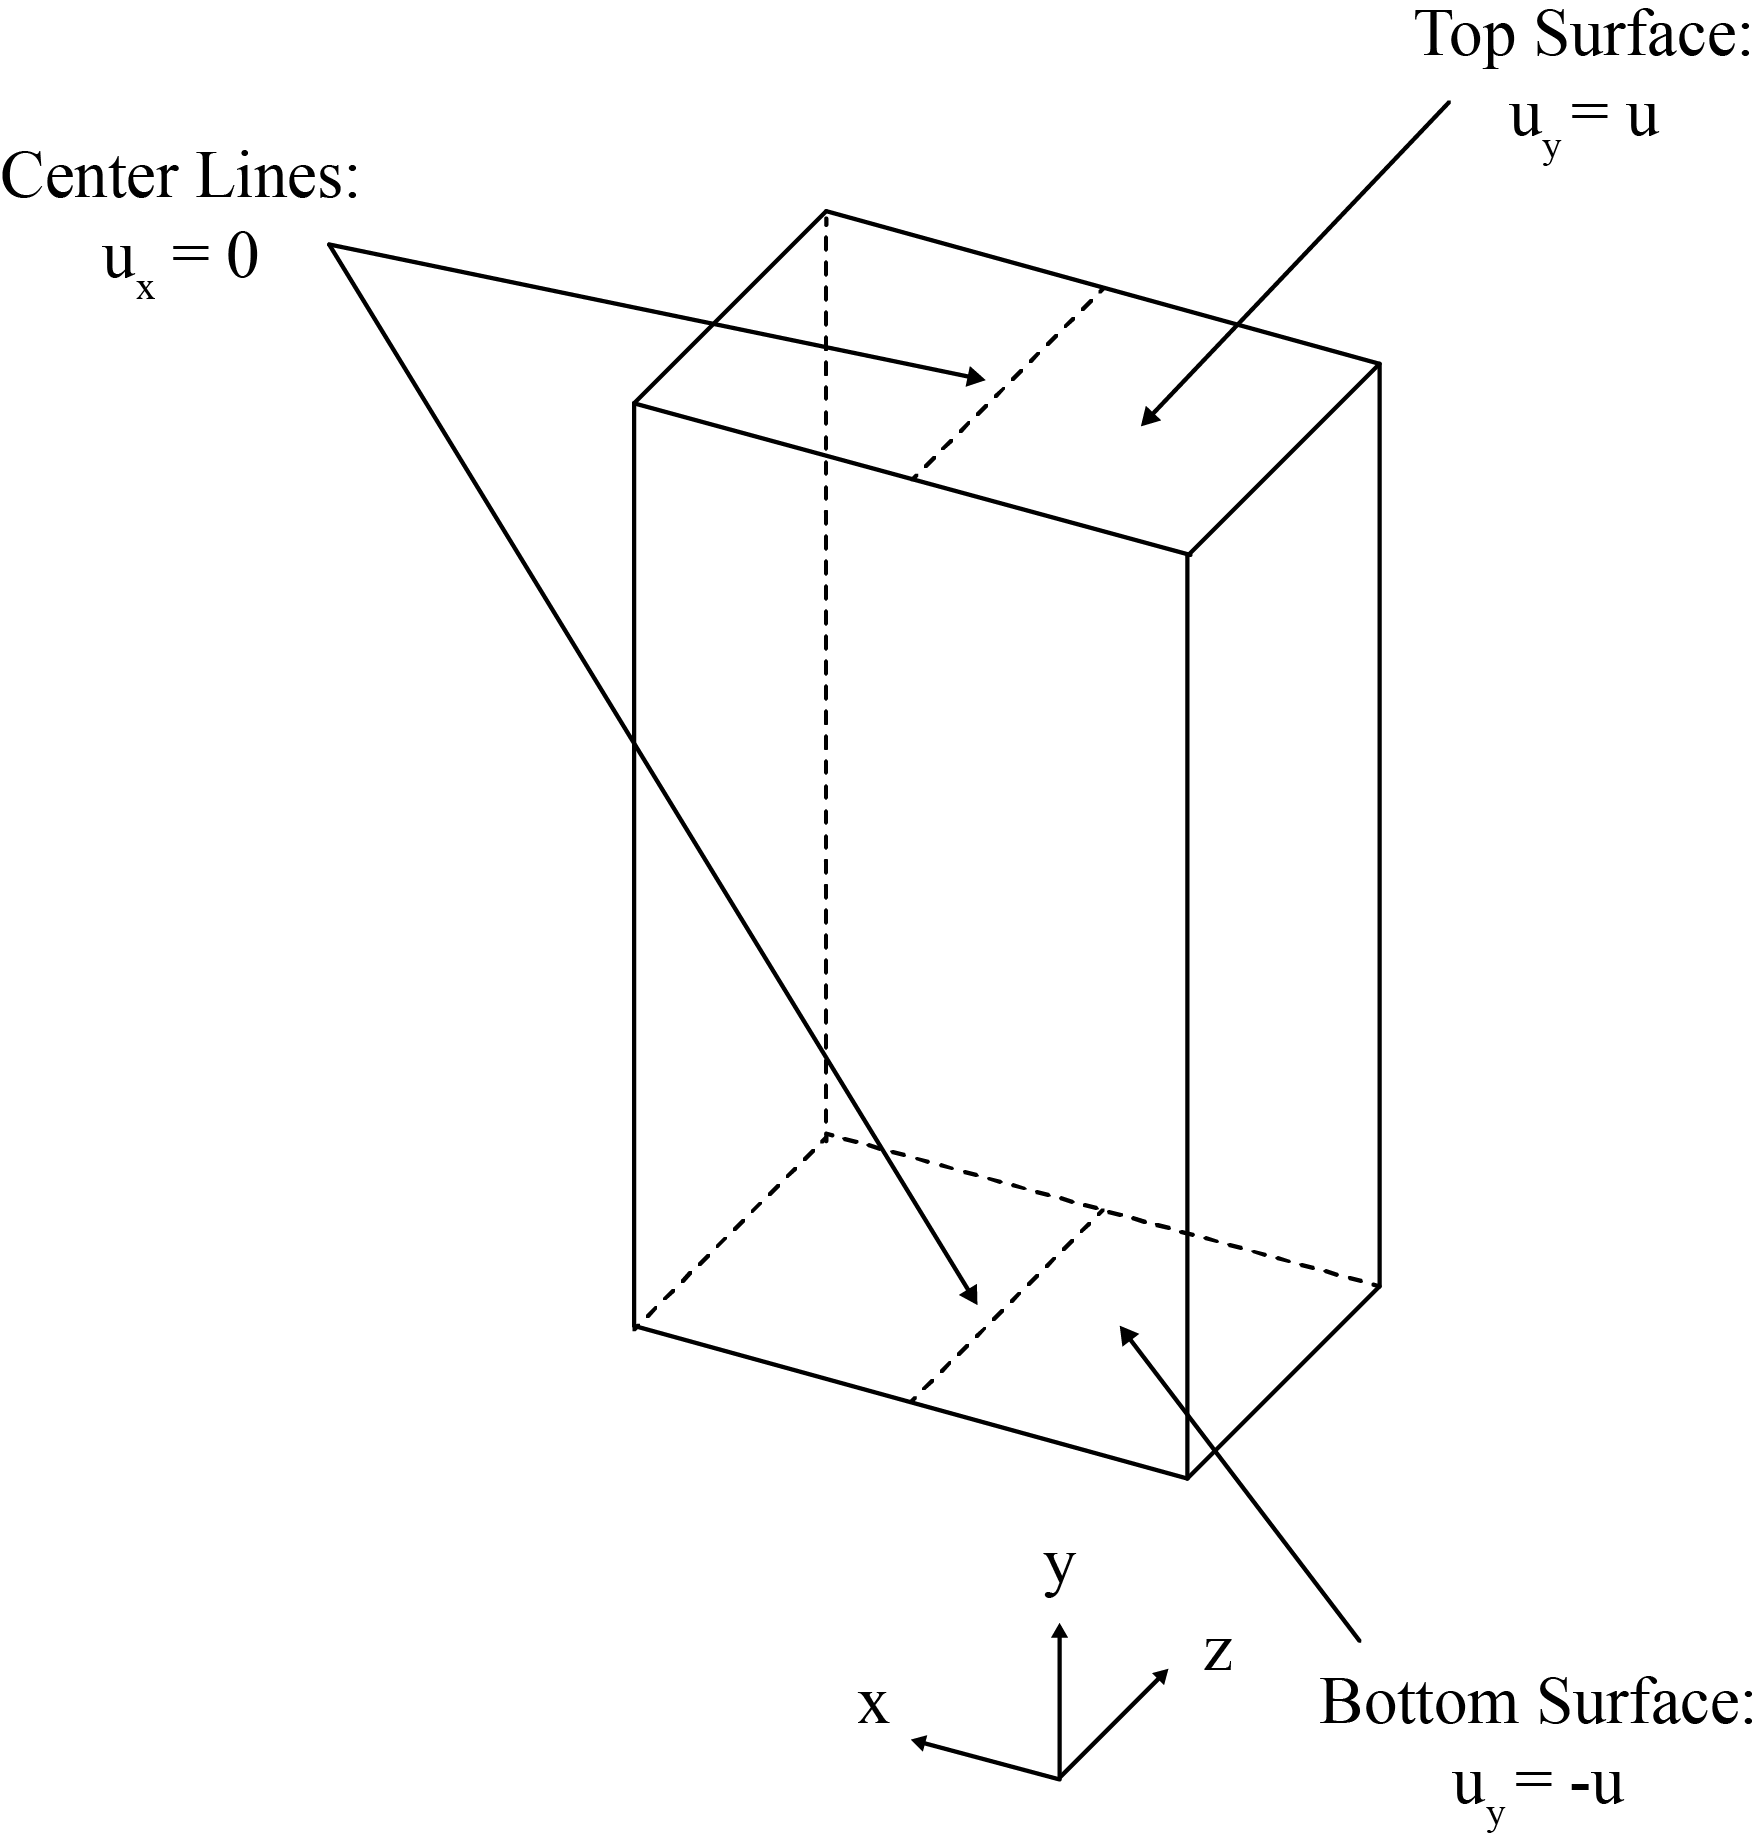
\includegraphics[width=4in]{geometry_figures/BCs.png} }}%
    \qquad
    \subfloat[\centering Model geometry]{{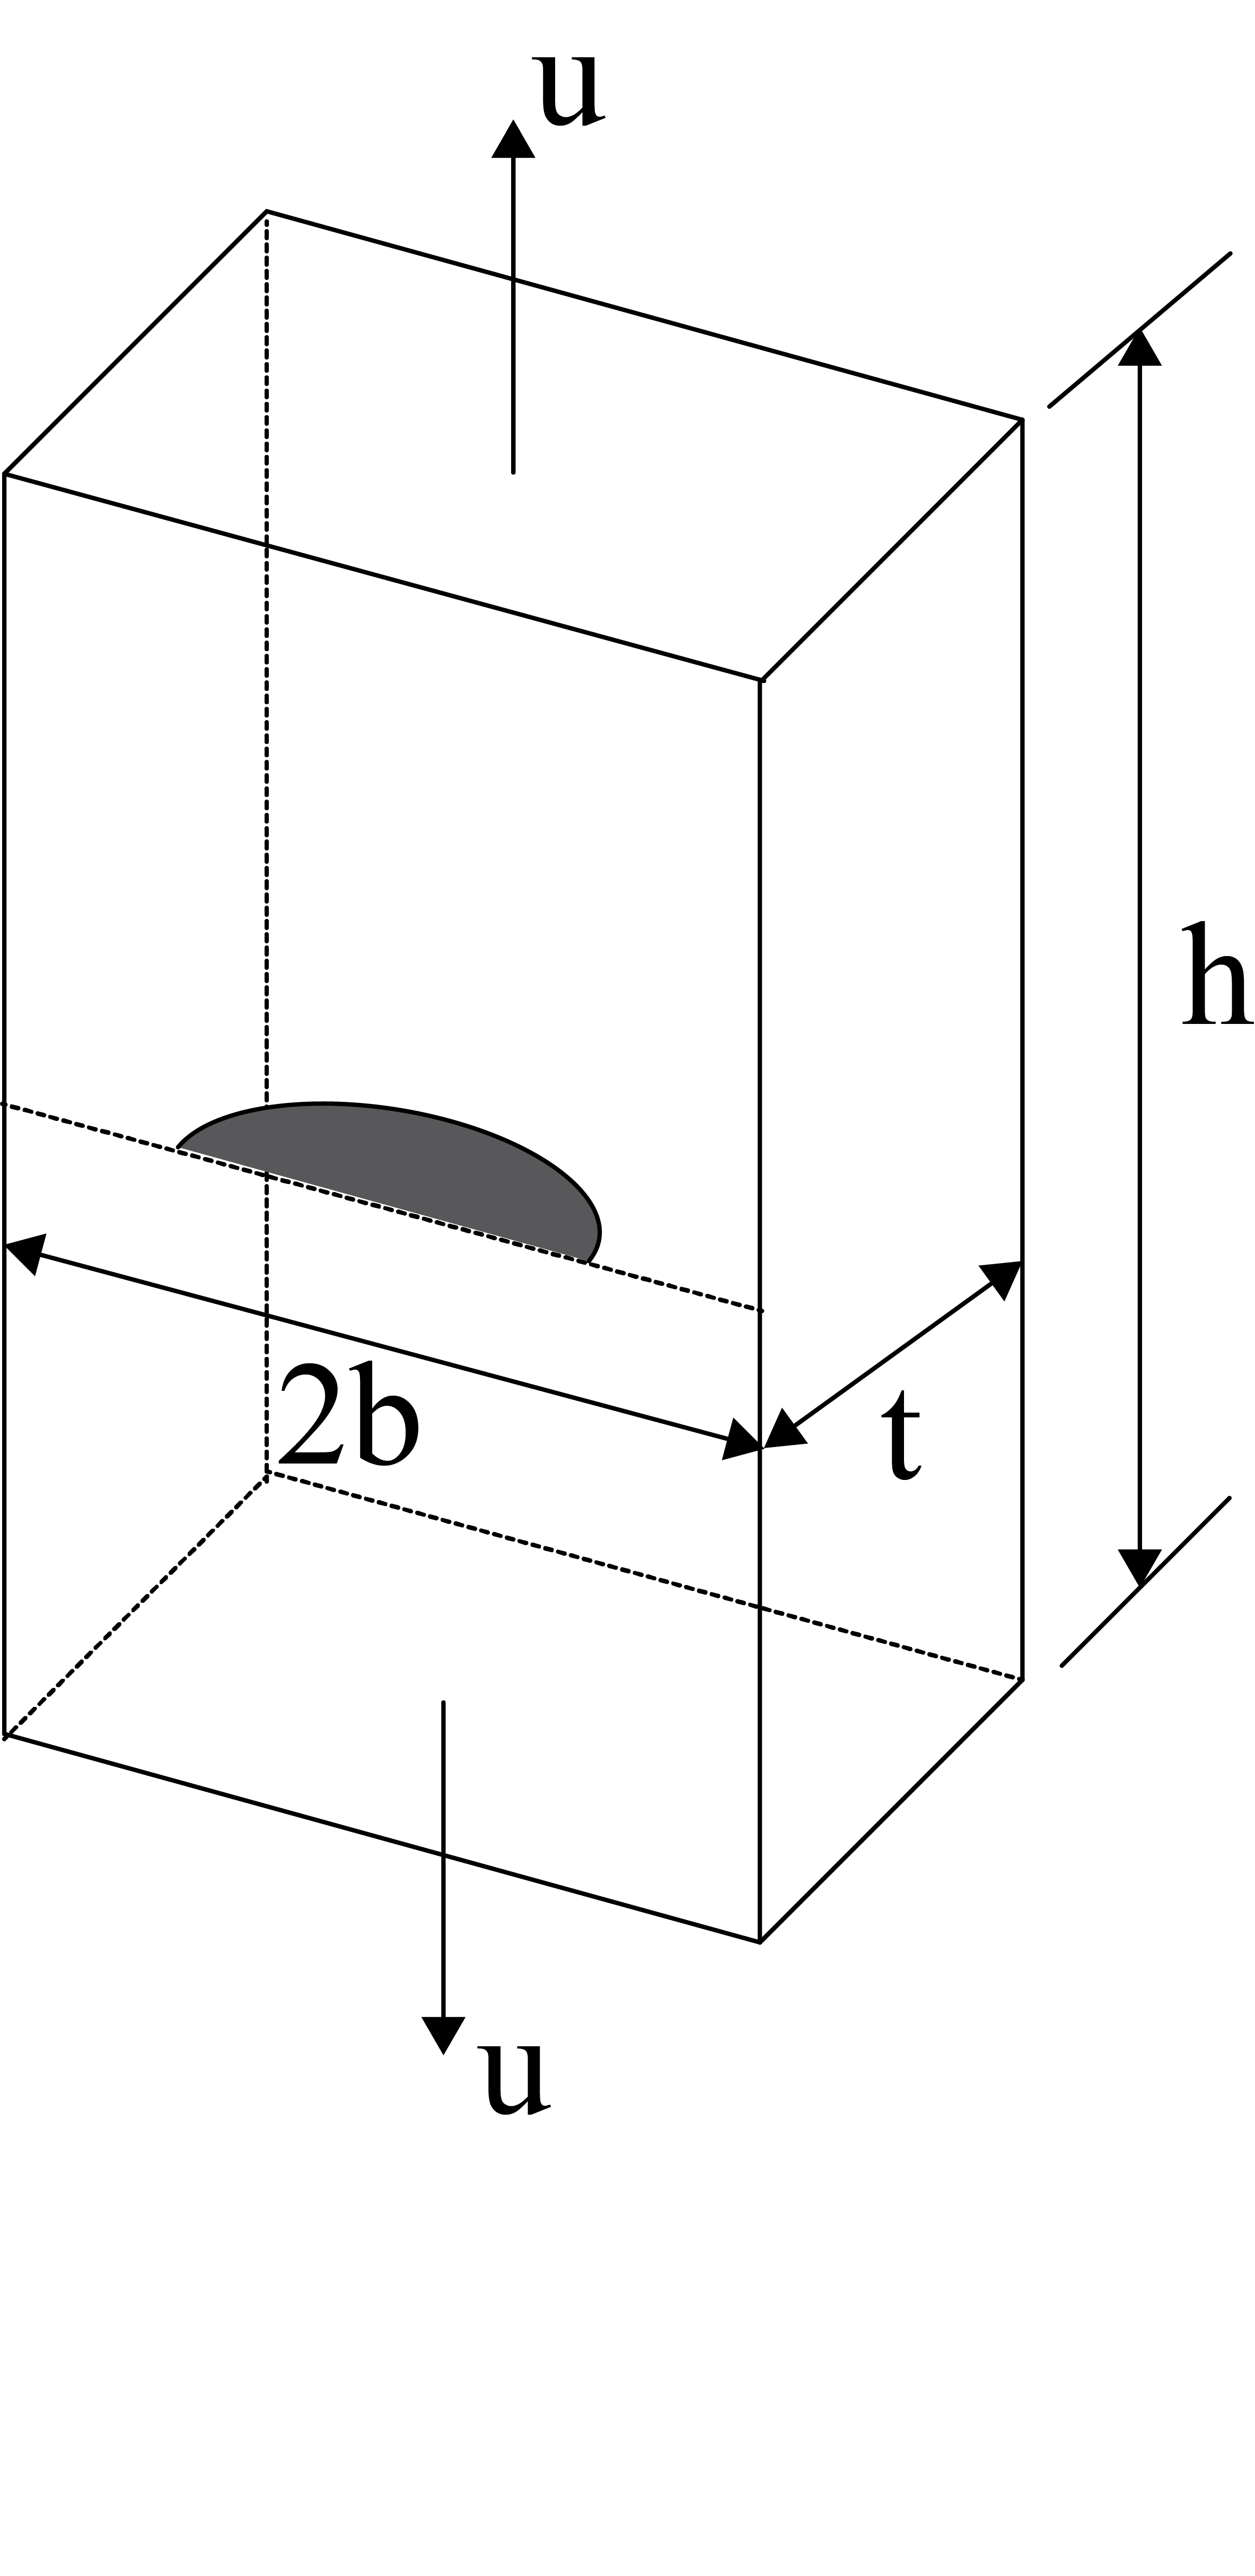
\includegraphics[width=2in]{geometry_figures/Geom.png} }}%
    \caption{(a) Top and bottom surfaces with displacement in $+y$ and $-y$ respectively. The center lines of the top and bottom faces are held $0$ in $x$. (b) Model geometry plate hight: $h$, plate width: $2b$, and plate thickness: $t$.}%
    \label{fig:model_params}%
\end{figure}

\begin{figure}%
    \centering
    \subfloat[\centering Crack dimensions]{{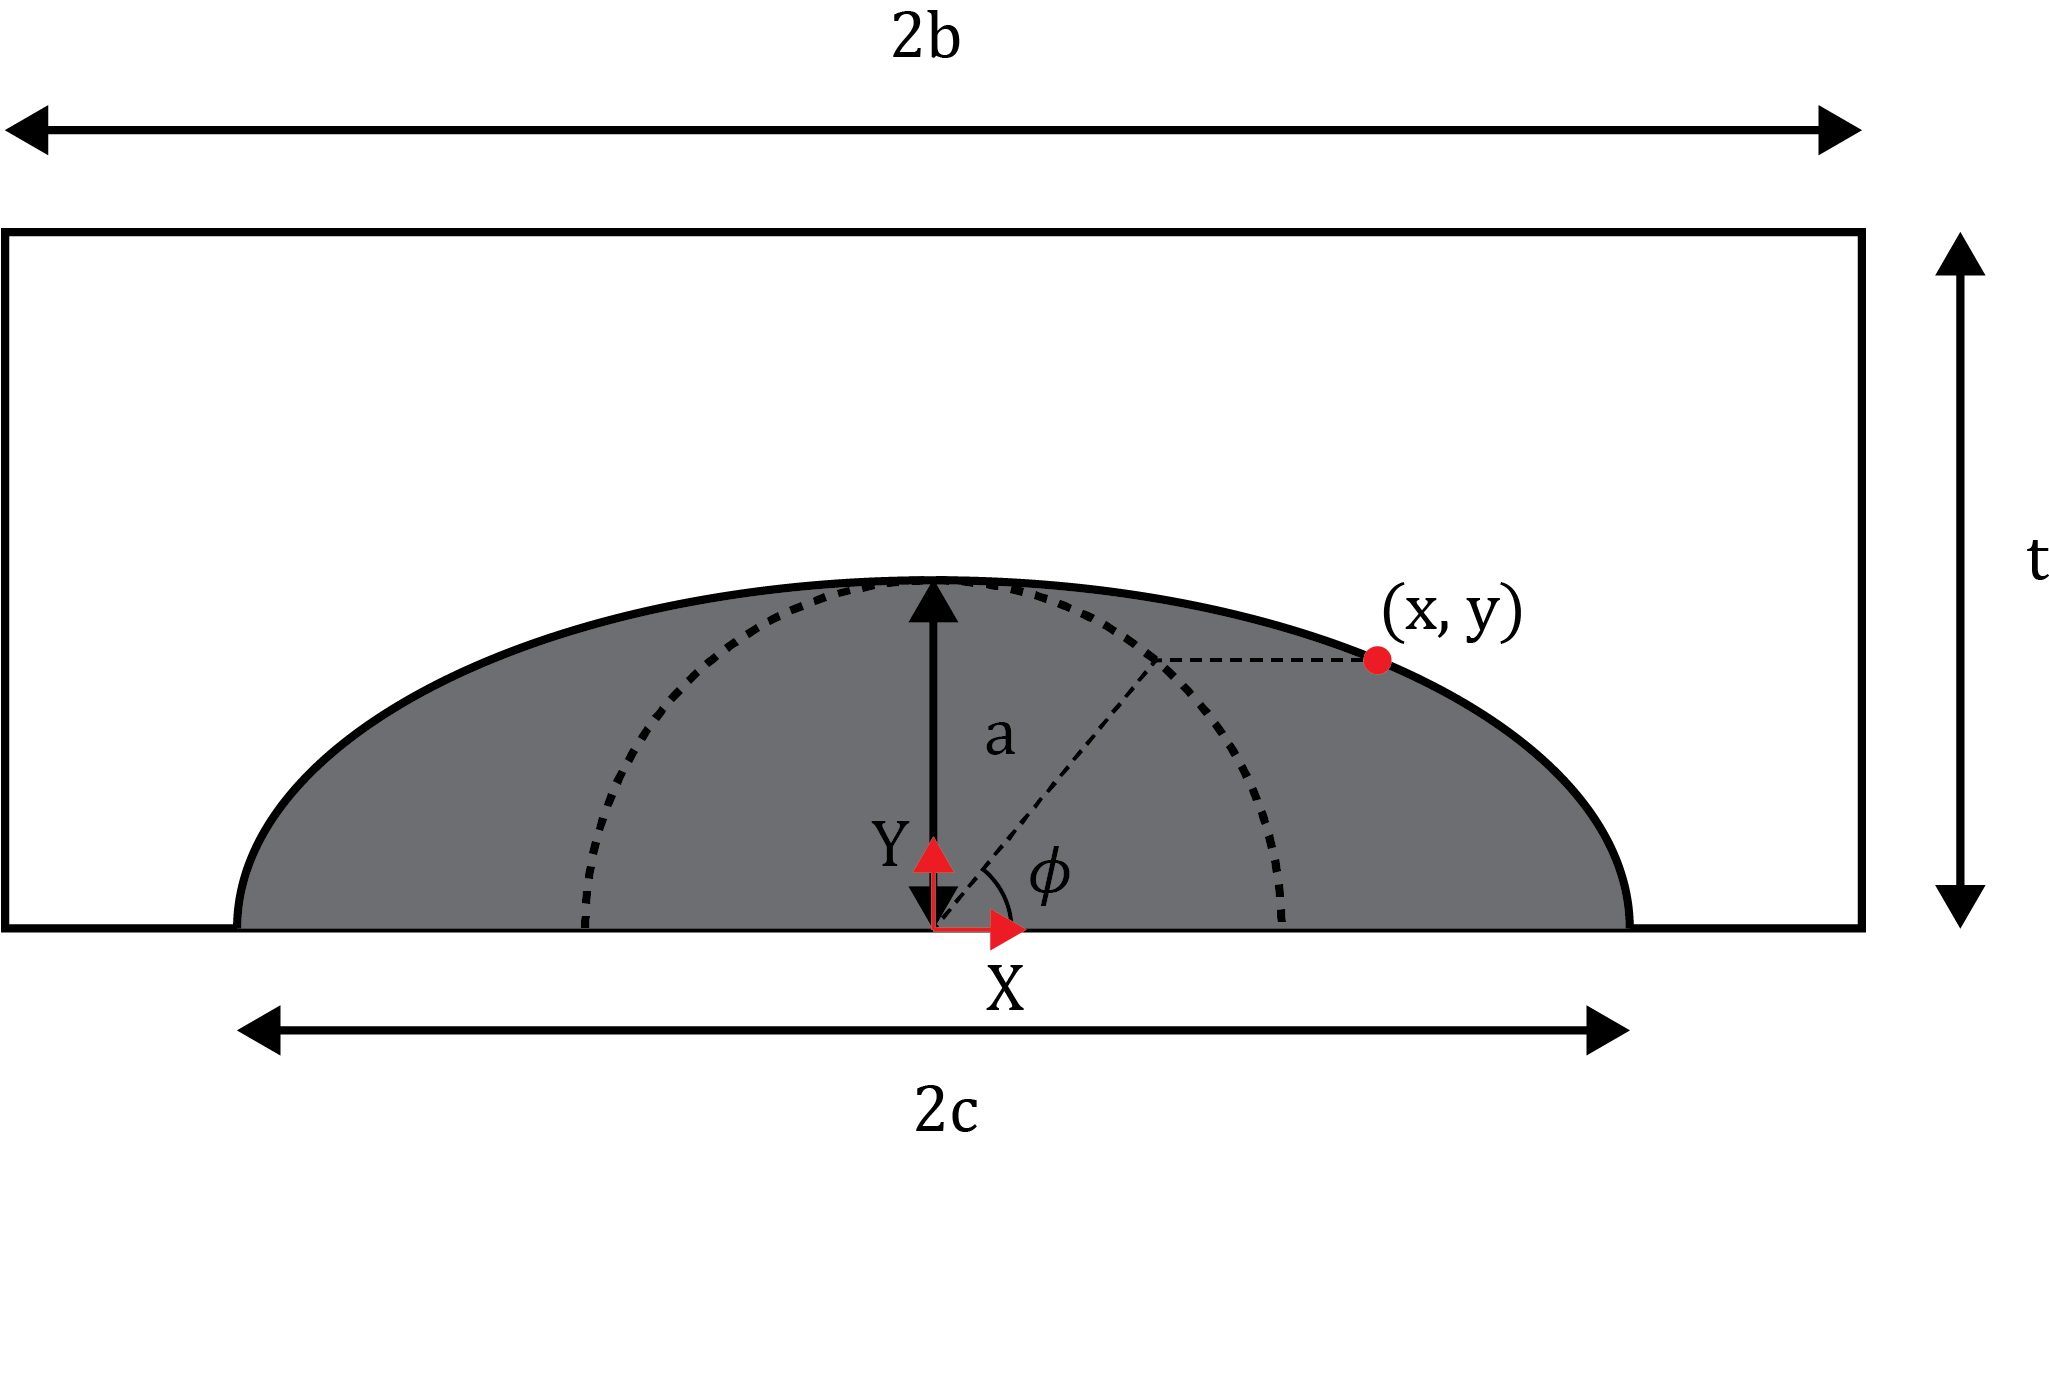
\includegraphics[width=3in]{geometry_figures/params.png} }}%
    \qquad
    \subfloat[\centering Ellipse dimensions]{{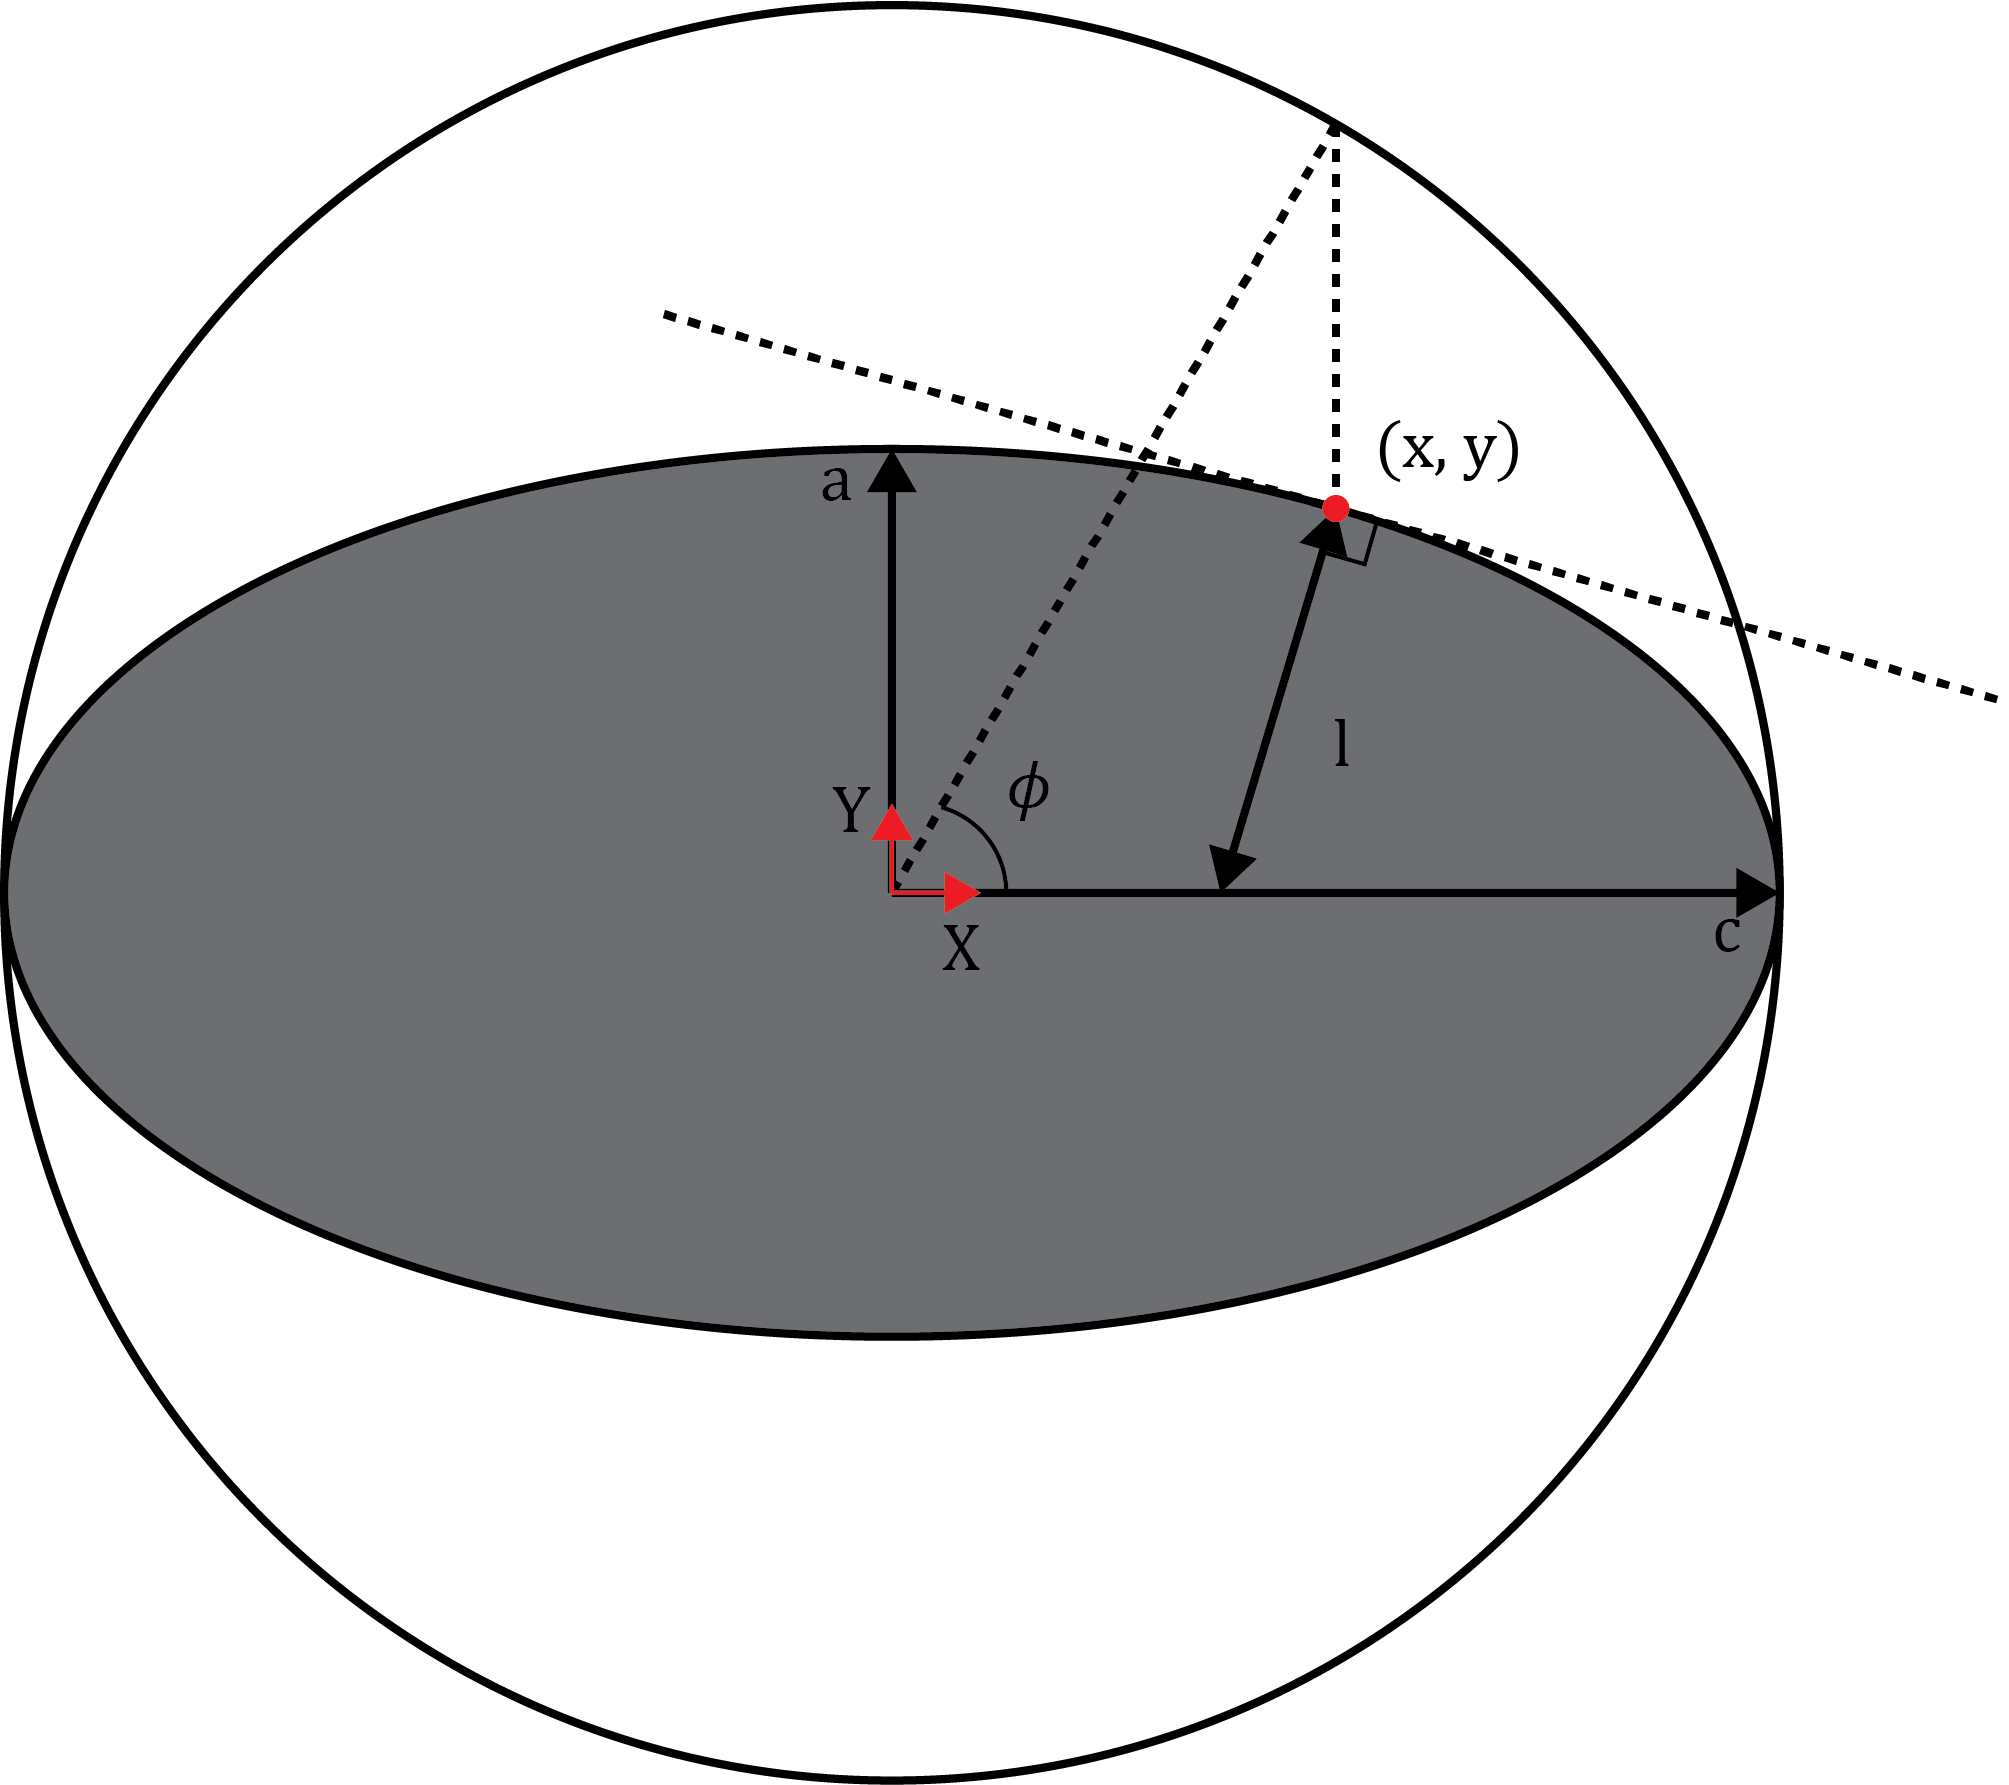
\includegraphics[width=3in]{geometry_figures/Ellipse.png} }}%
    \caption{(a) Crack pameters with $a$ being the crack depth and $2c$ being the surface crack length. (b) $\phi$ is defined by the angle to the enscribed circle projected to the ellipse. $l$ is defined as the distance perpendicular to the tangent line from the point of interest to the nearest axis.}%
    \label{fig:crack_params}%
\end{figure}


\begin{figure}%
    \centering
    \subfloat[\centering Convergence of $h/t$]{{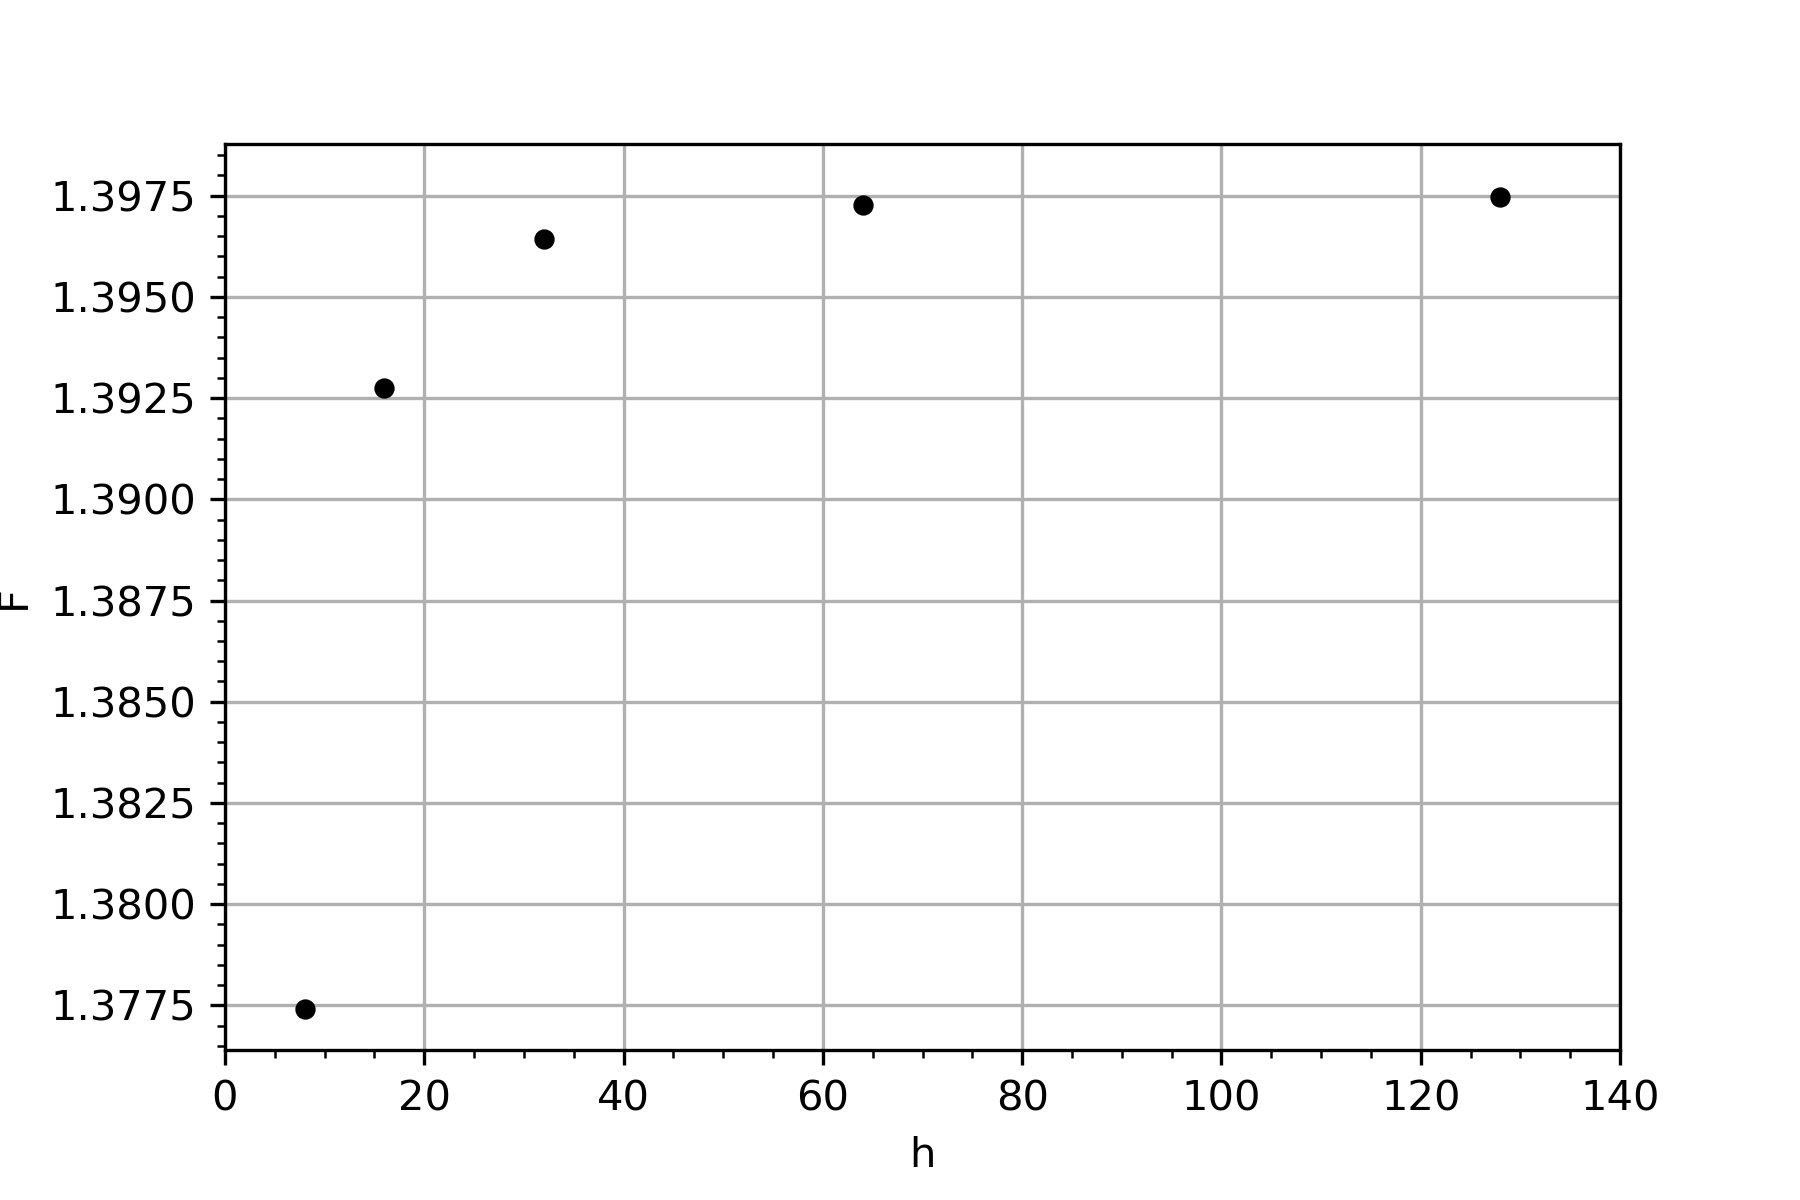
\includegraphics[width=3in]{Figures/h_convergence.png} }}%
    \qquad
    \subfloat[\centering convergence of $c/b$]{{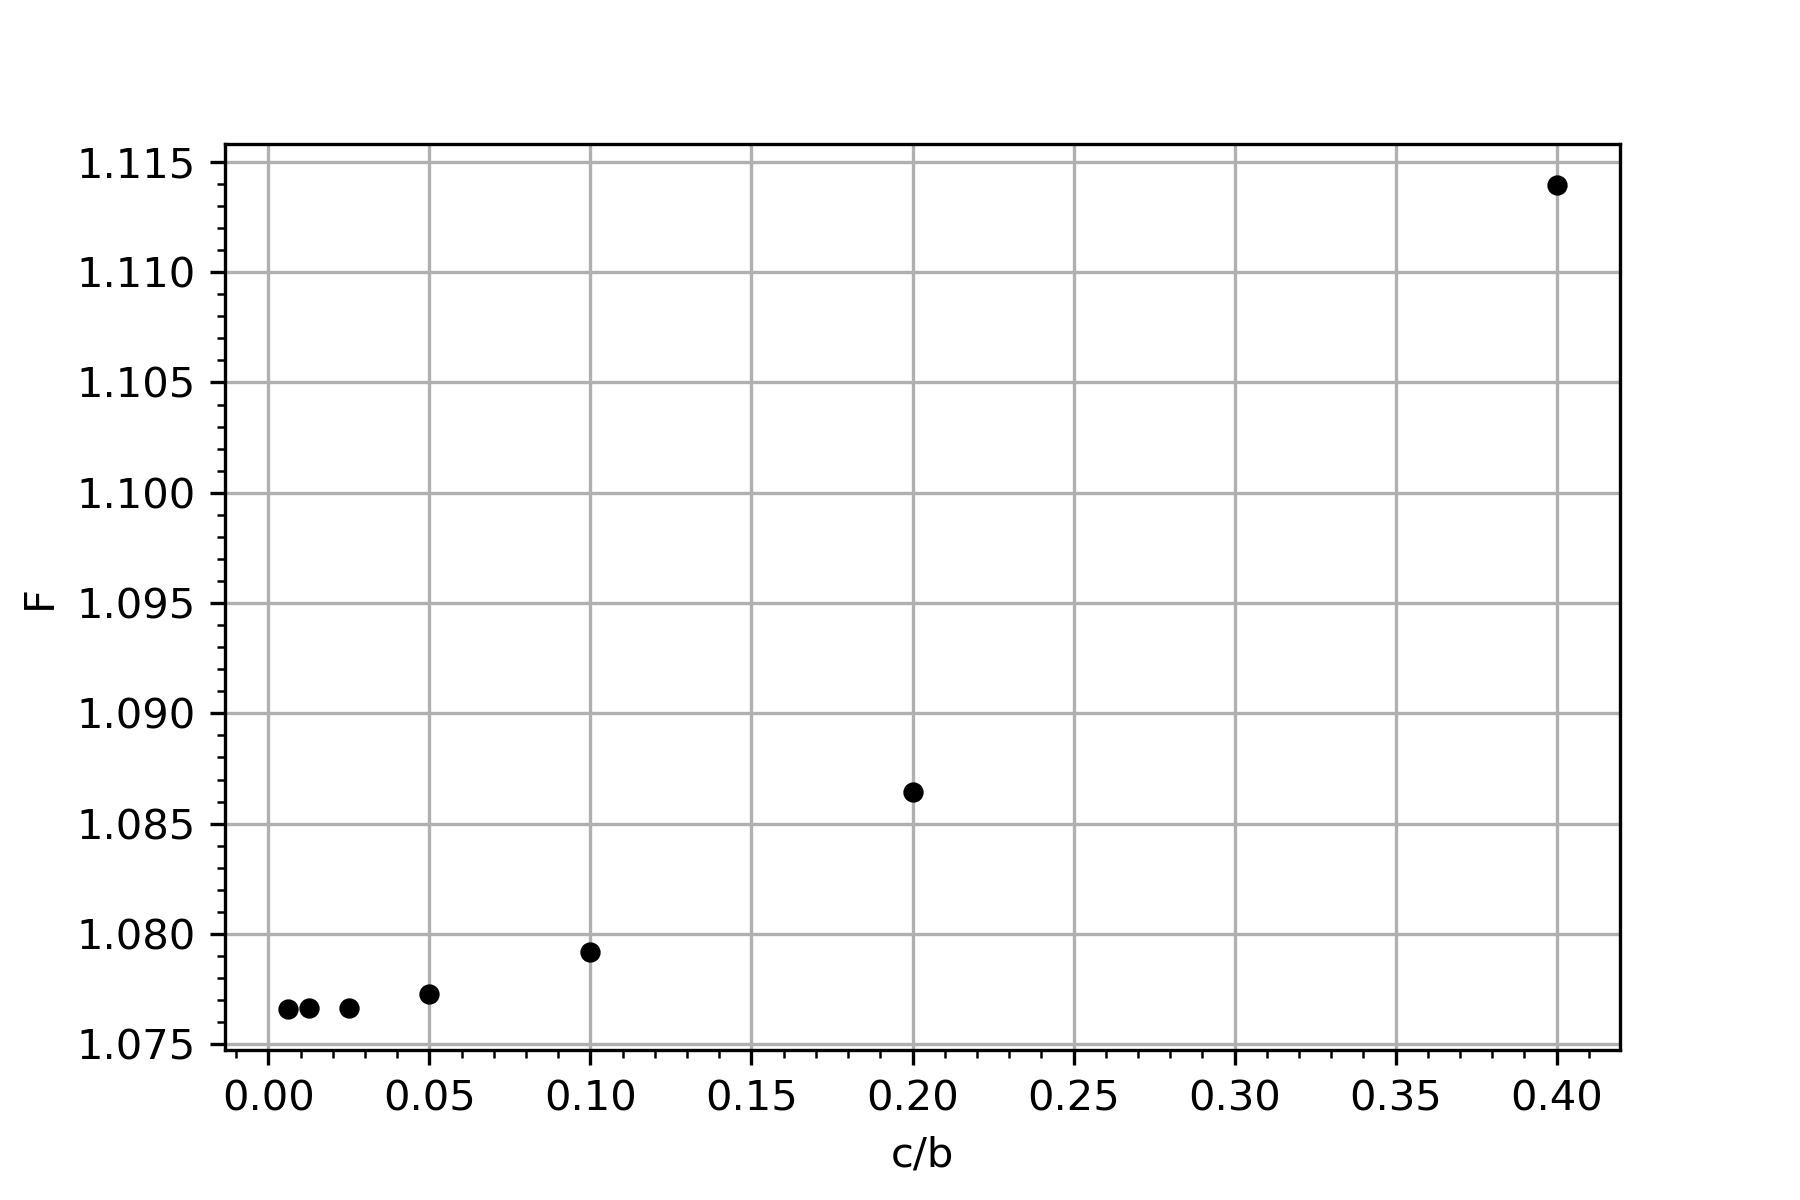
\includegraphics[width=3in]{Figures/cb_convergence.png} }}%
    \caption{(a) the convergence of $h/t$ is plotted using the mean boundary correction factor (b) The convergence of $c/b$ is plotted using the mean boundary correction factor.}%
    \label{fig:convergence_plots}%
\end{figure}


\begin{figure}
    \centering
    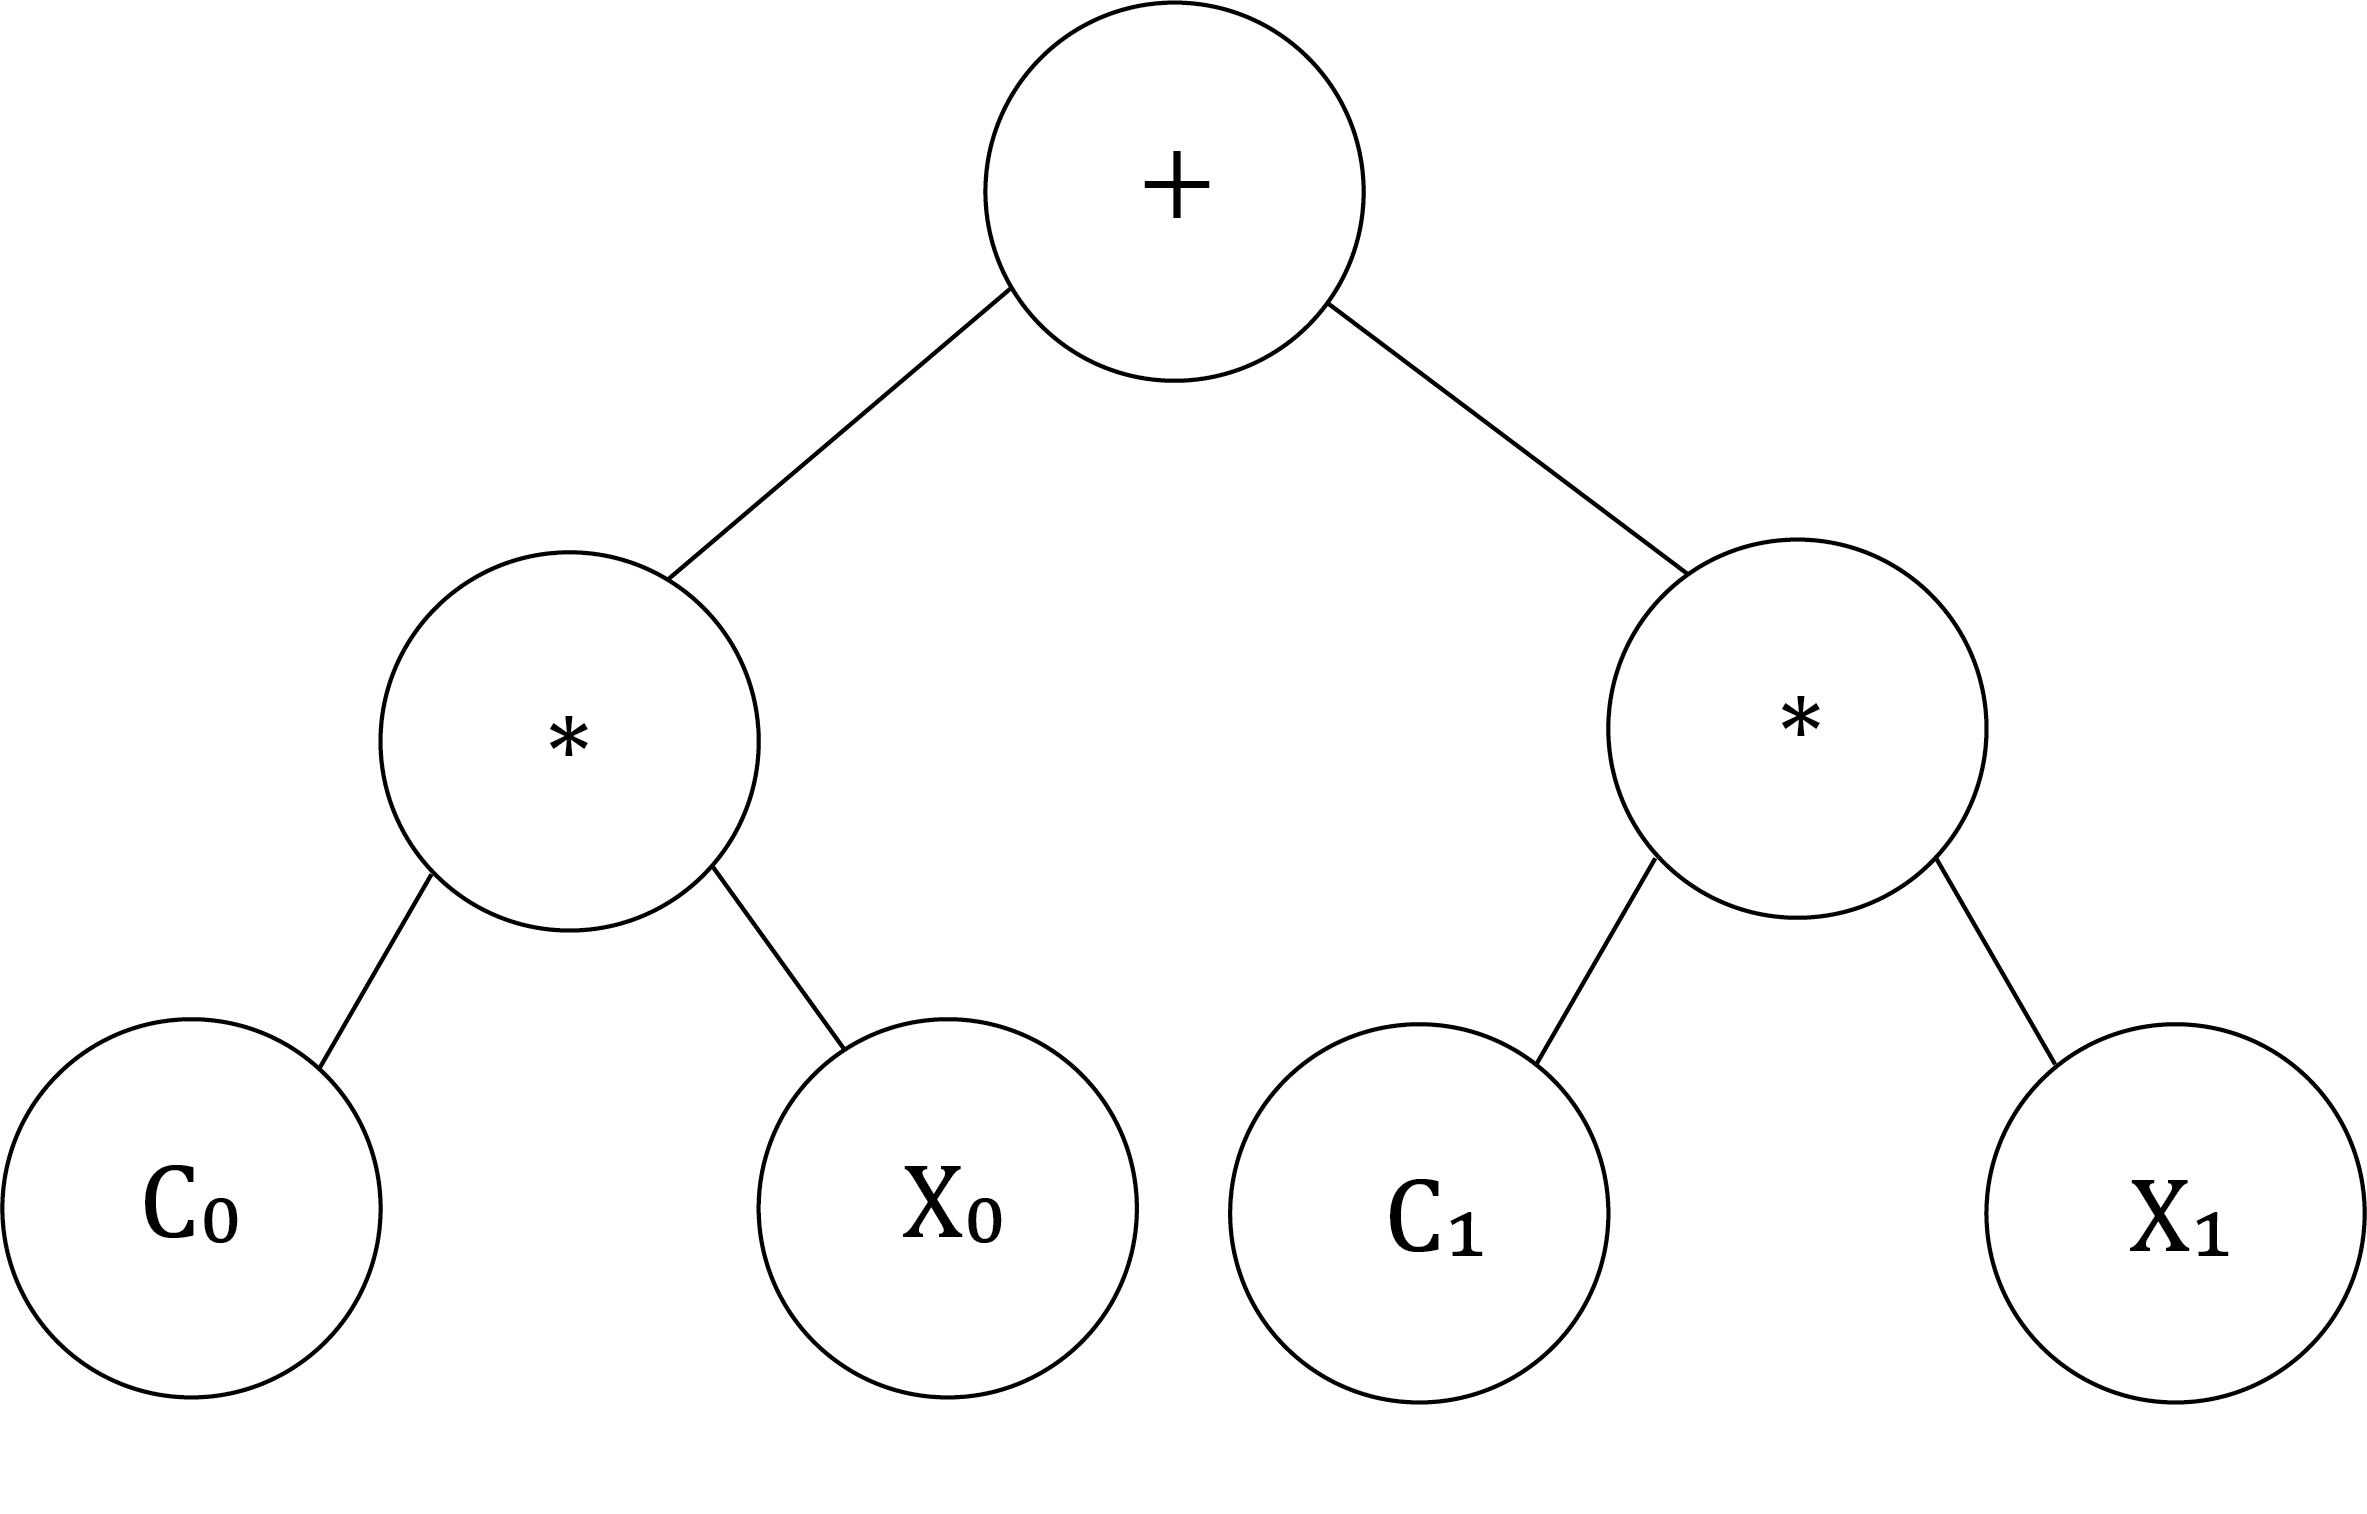
\includegraphics[width=4in]{geometry_figures/agraph.png}
    \label{fig:agraph}
    \caption{Example Agraph for for equation; $C_0 X_0 + C_1 X_1$, where the complexity is the sum of the nodes in this case 7.} 
\end{figure}


\begin{figure}%
    \centering
    \subfloat[\centering Distributions of error]{{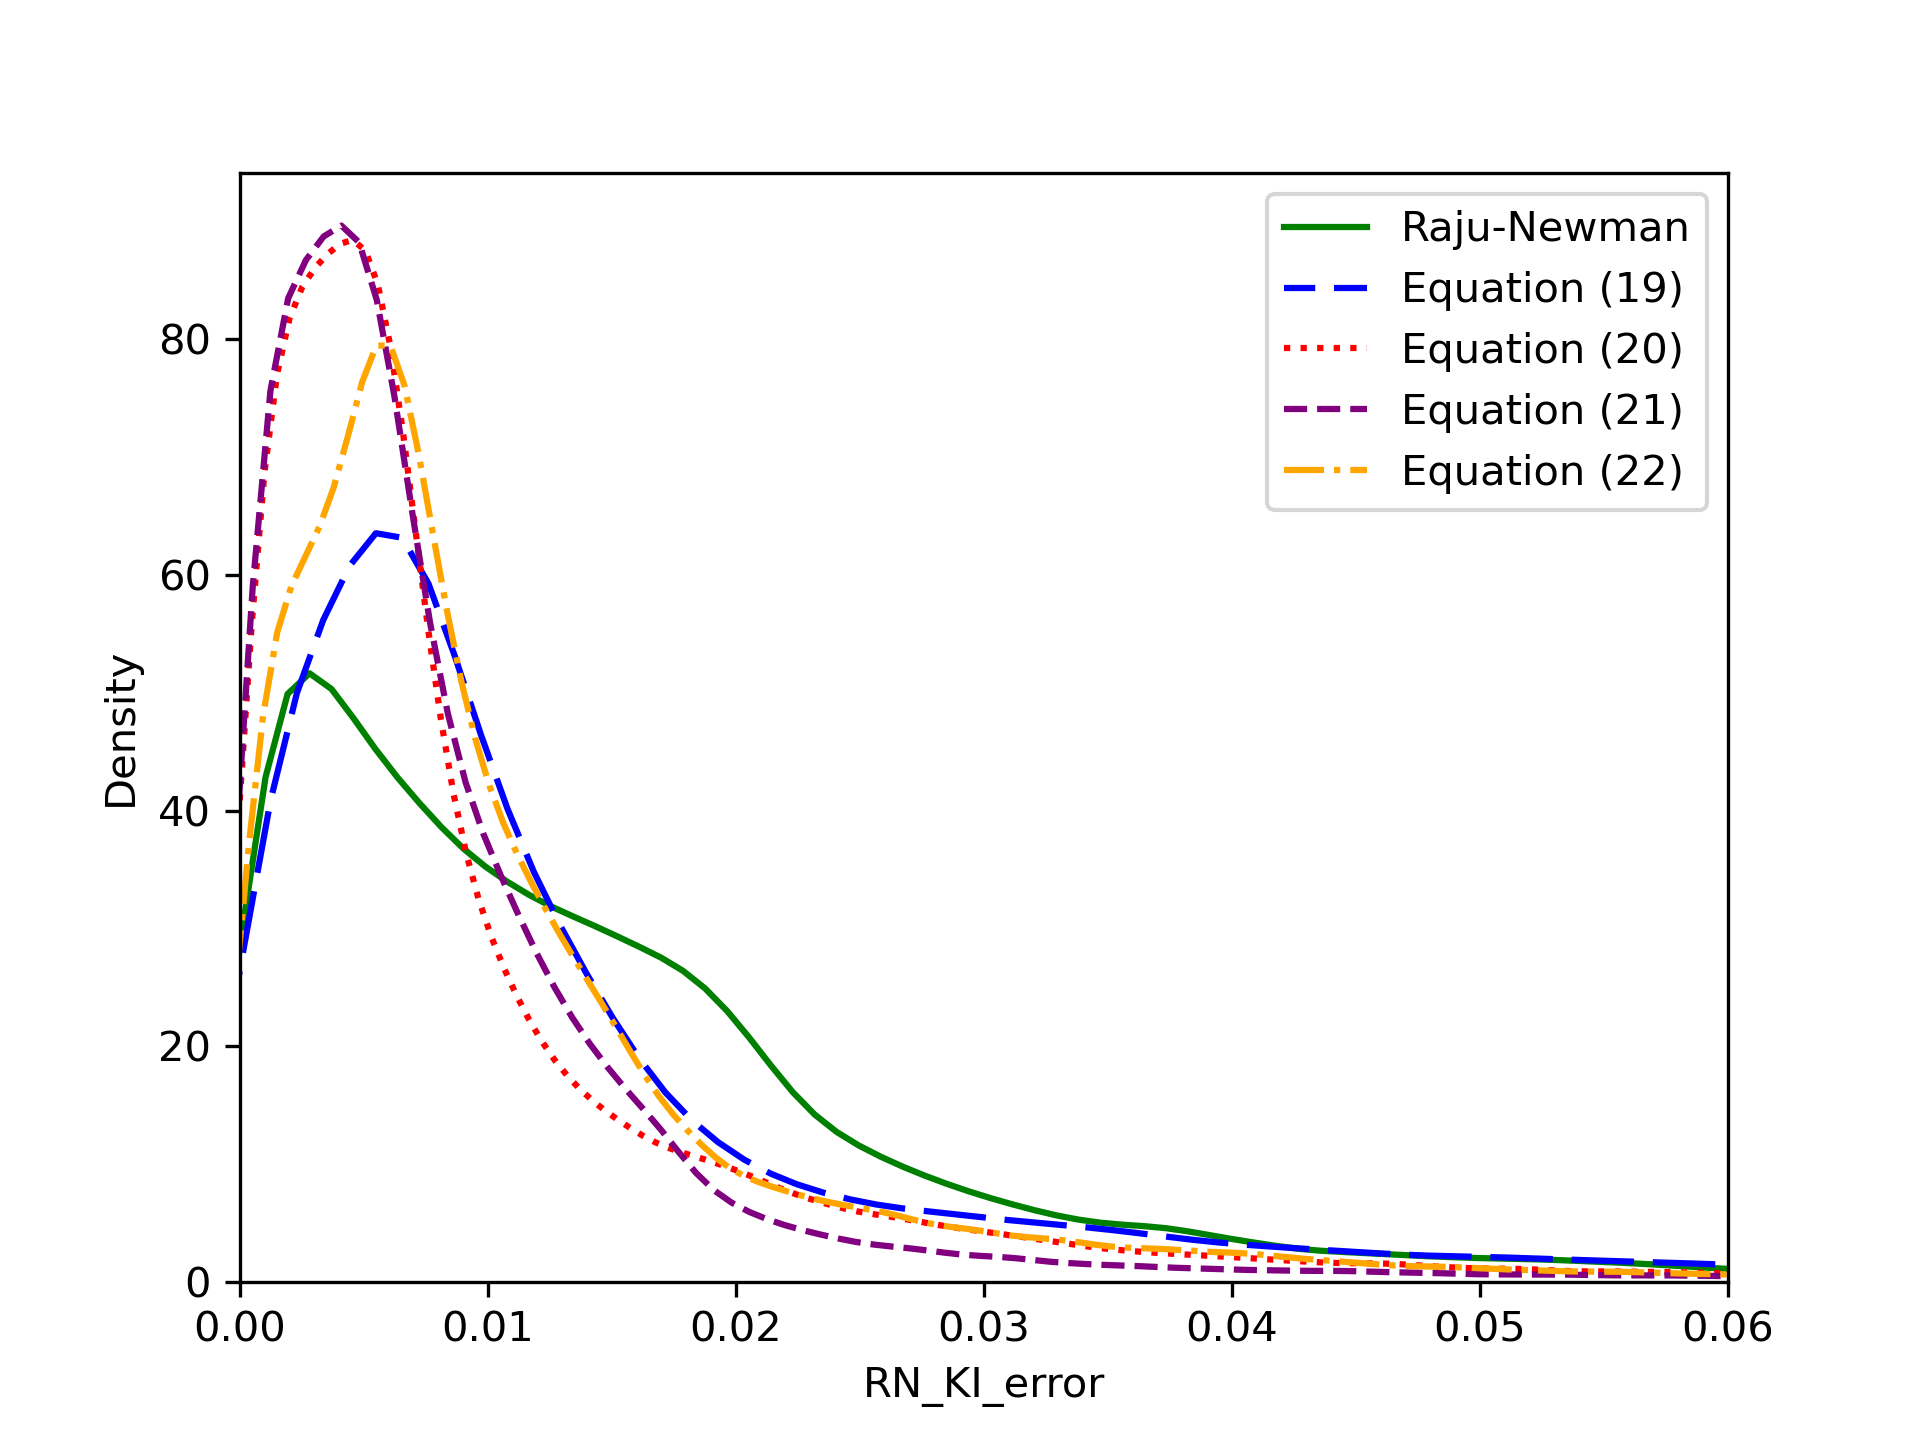
\includegraphics[width=3in]{Figures/kde_plot.png} }}%
    \qquad
    \subfloat[\centering Parity plots]{{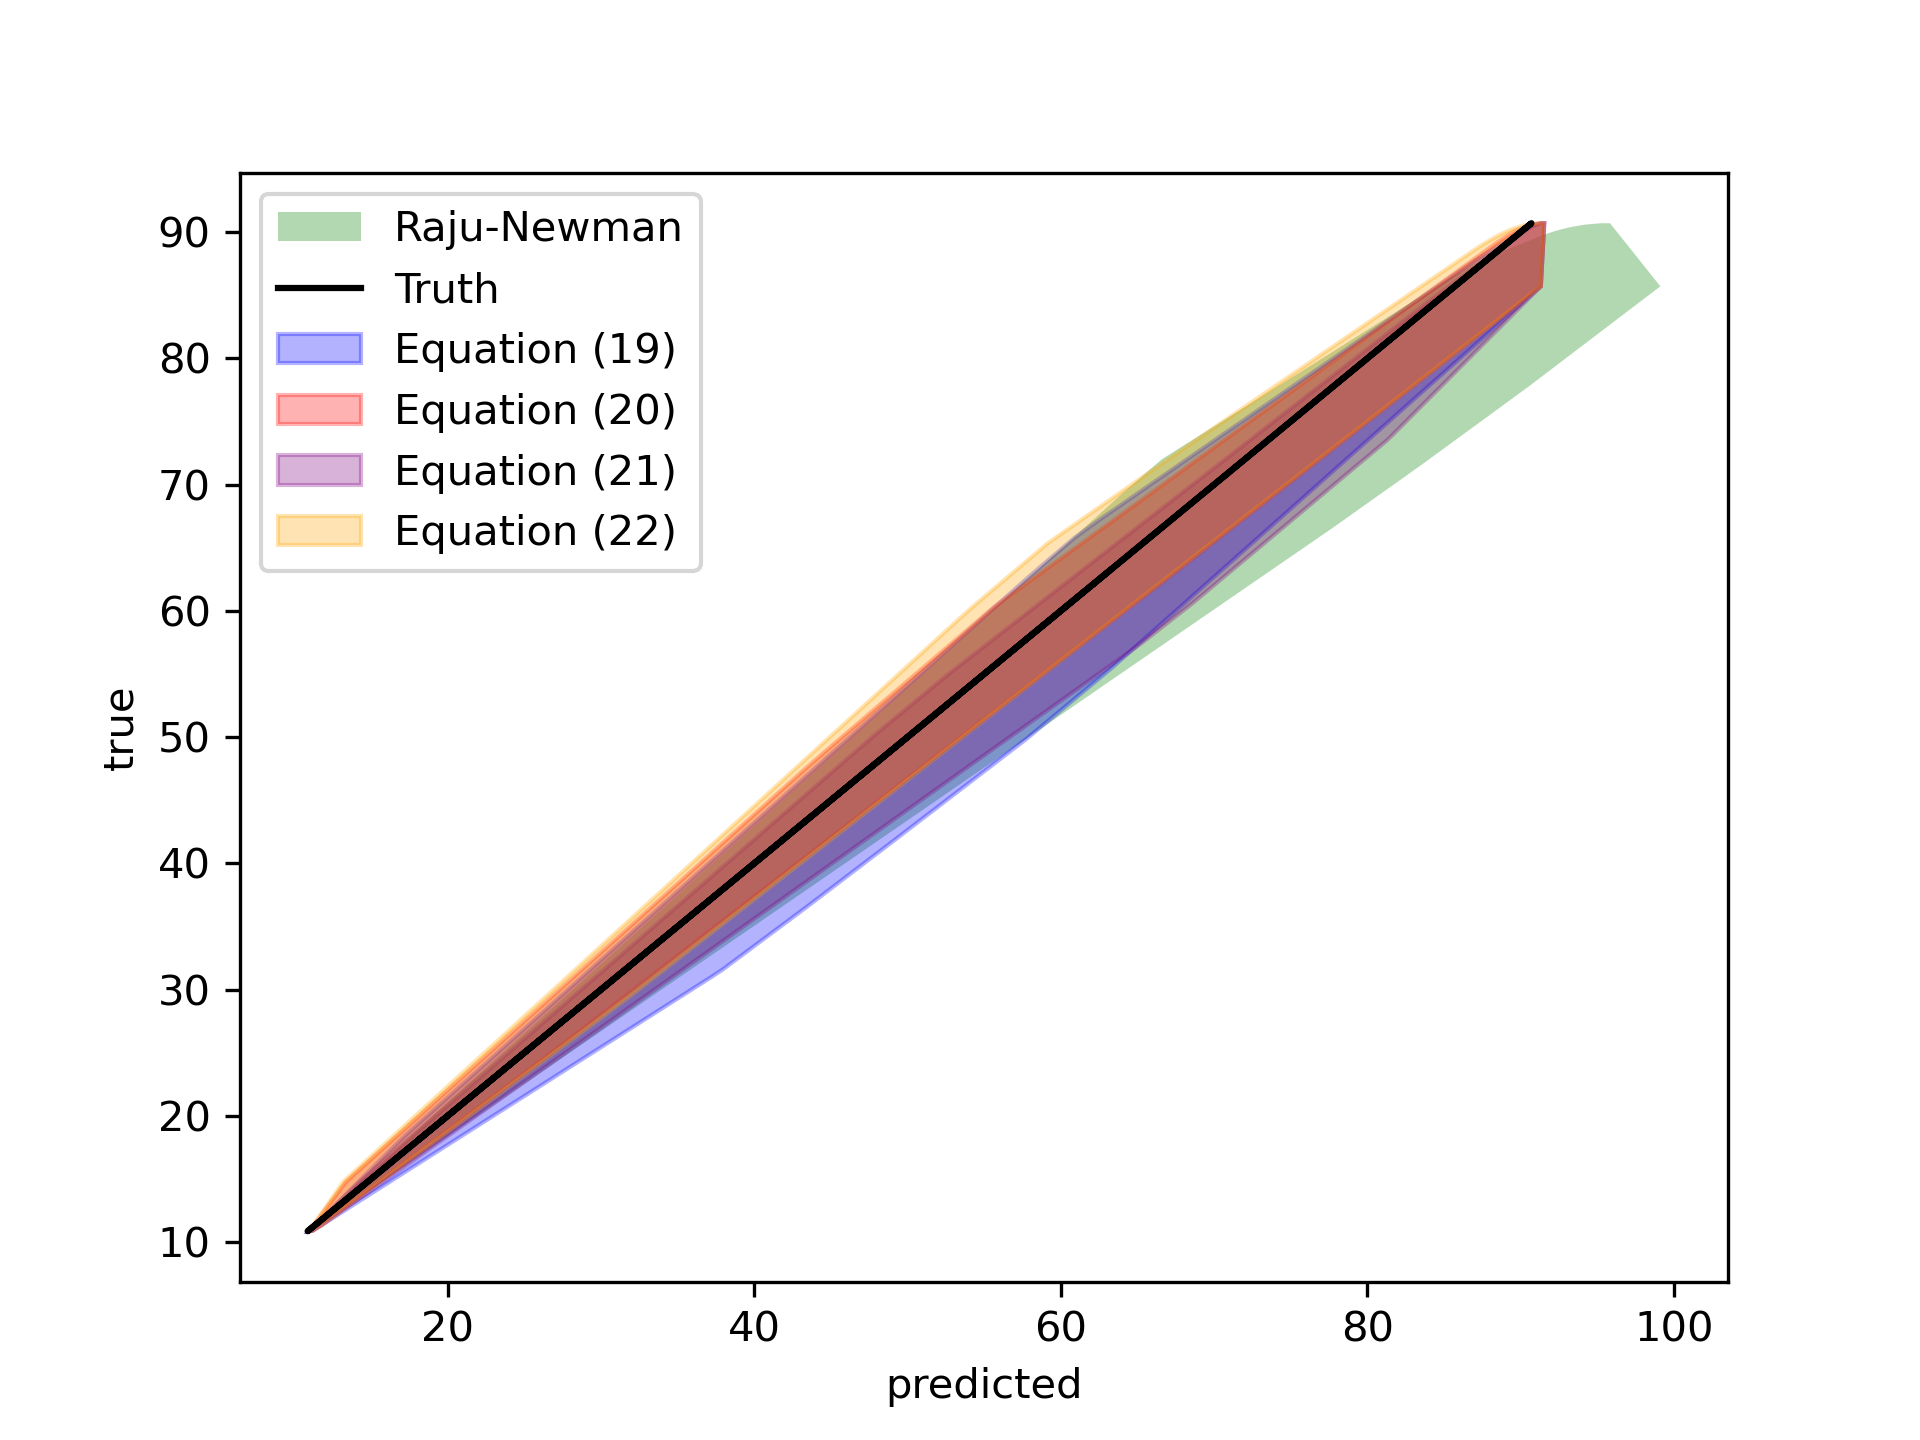
\includegraphics[width=3in]{Figures/parity_plot.png} }}%
    \caption{(a) Density plot for the errors of each of the equations. (b) Parity plot with each of the different equations.}%
    \label{fig:error_plots}%
\end{figure}


\begin{figure}
    \centering
    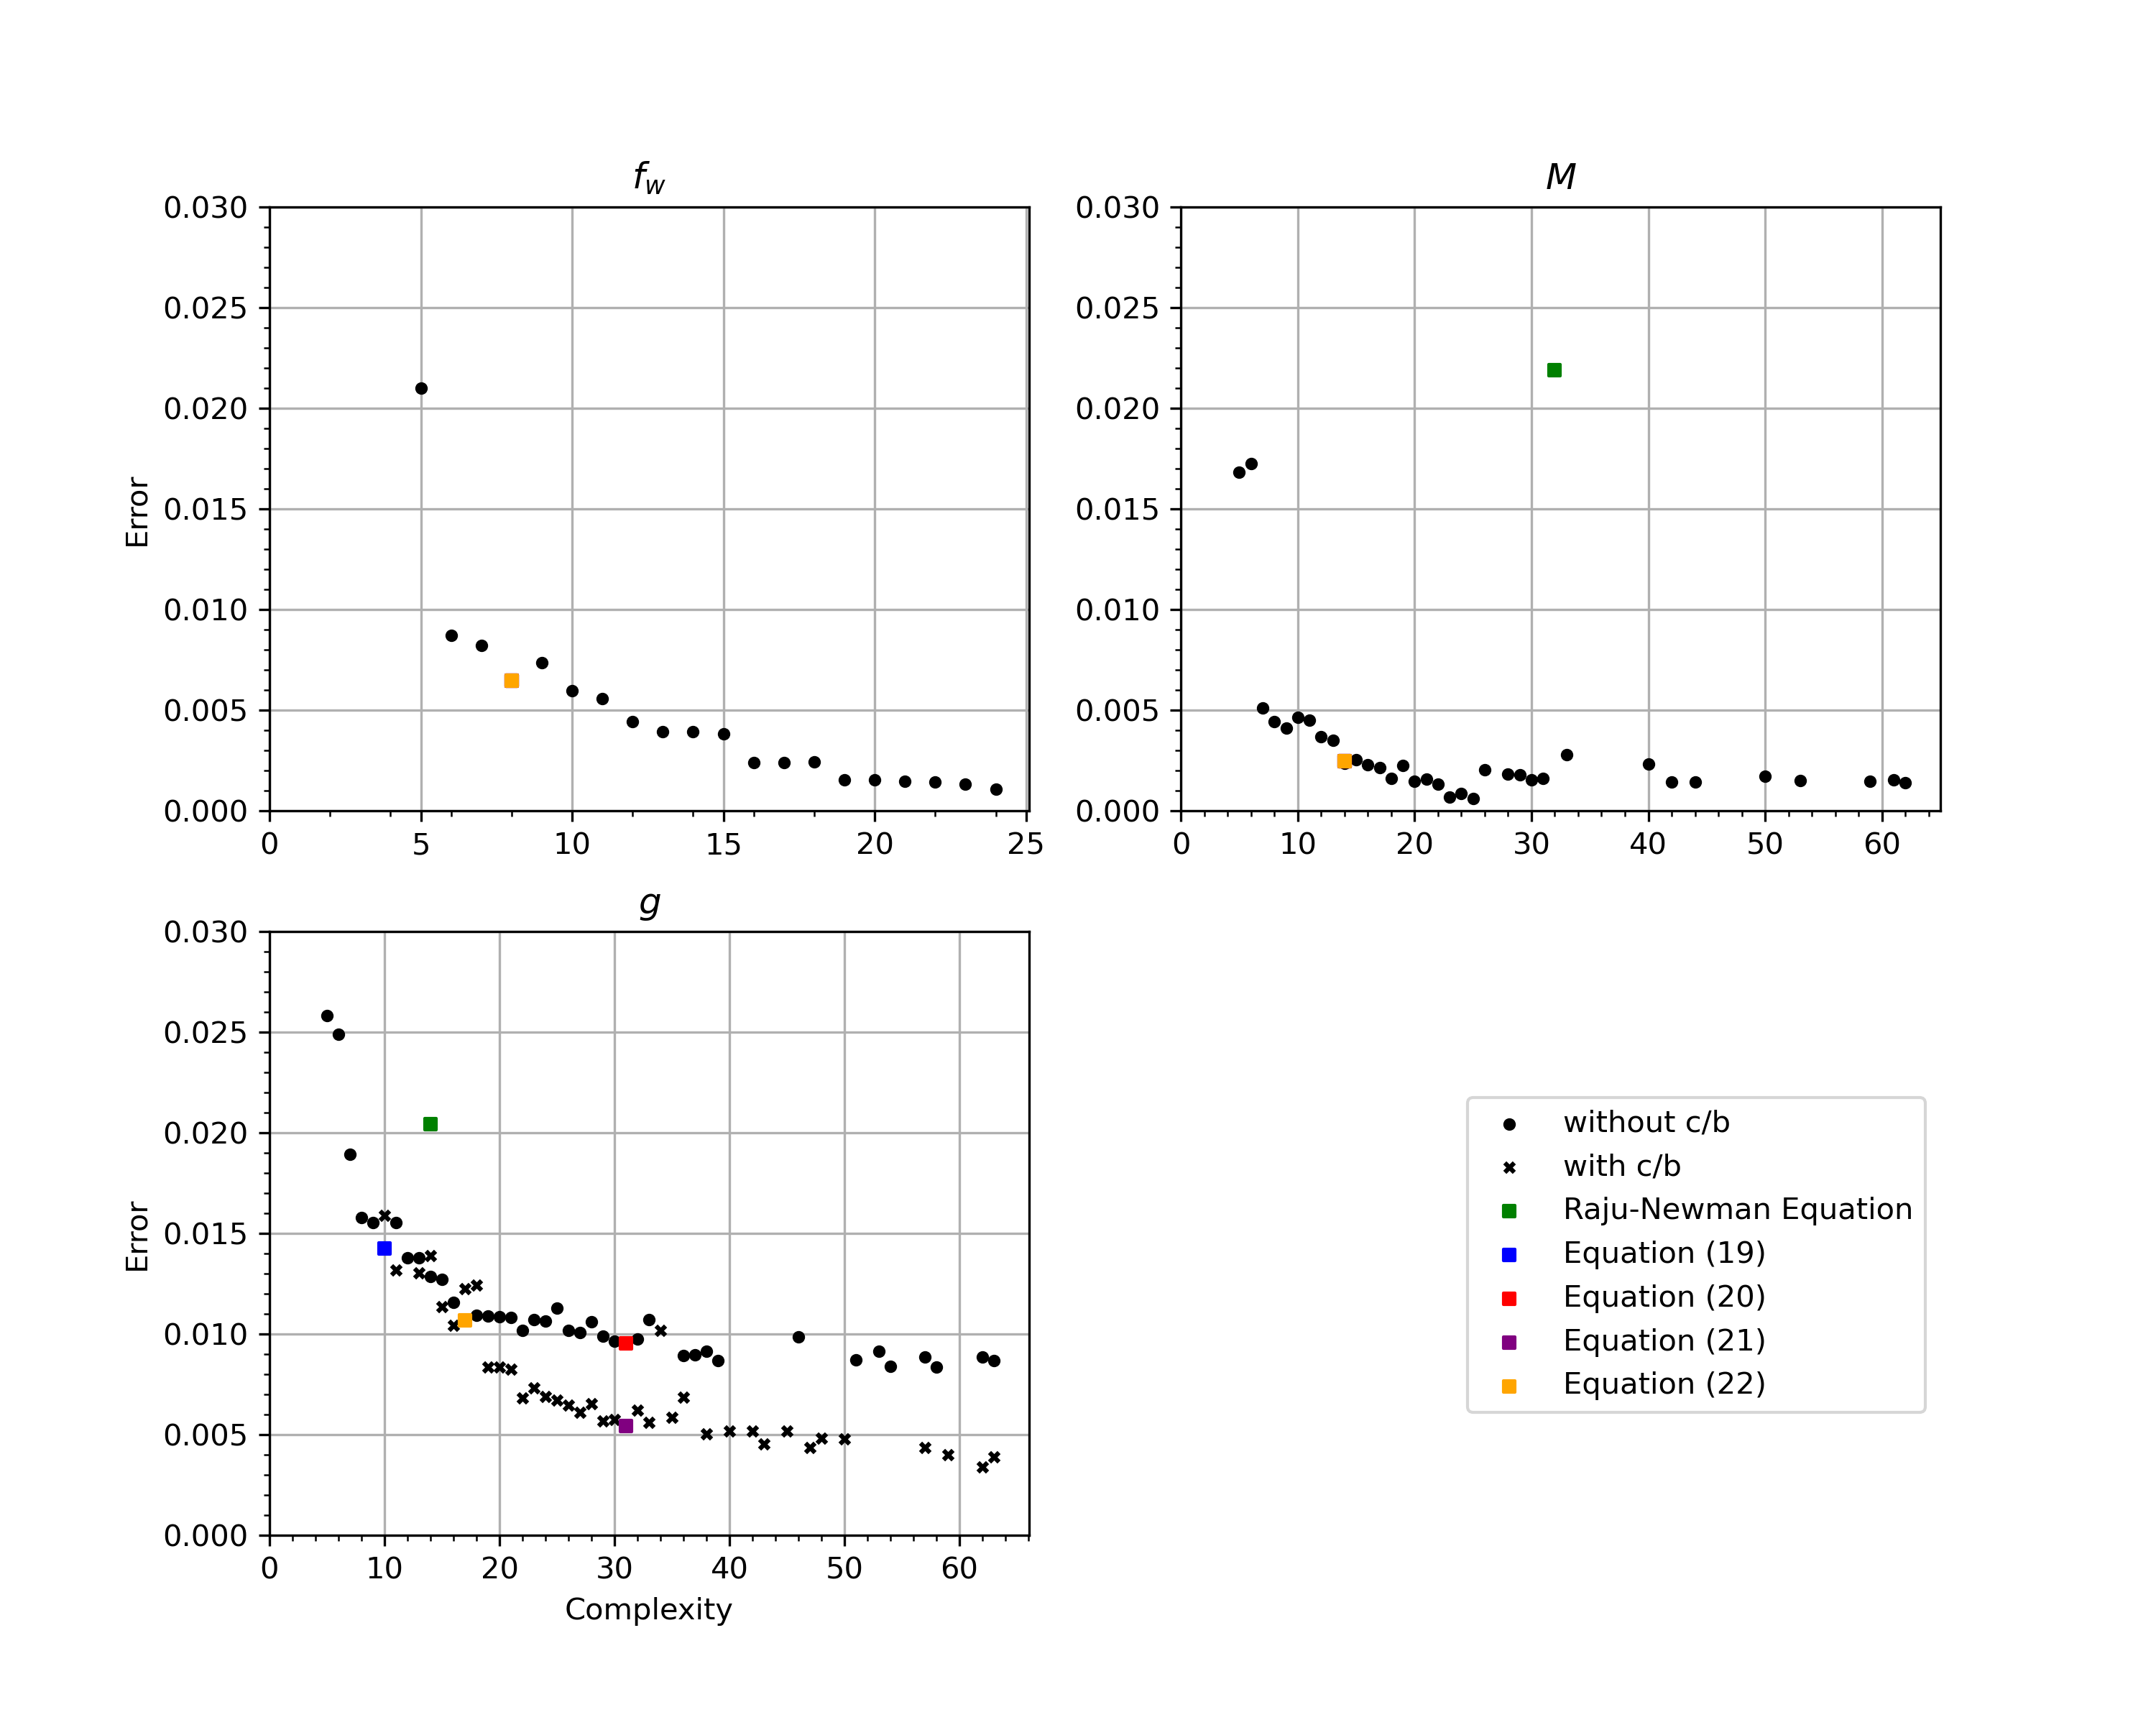
\includegraphics[width=6in]{Figures/perato_front.png}
    \label{fig:perato_front}
    \caption{Perato fronts for $f_w$, $M$, and $g$. $f_w$ and $M$ have the same equation for all four models. Both the perato fronts for $g$ with and without $c/b$ are shown} 
\end{figure}

\begin{figure}%
    \centering
    \subfloat[\centering Distributions of error]{{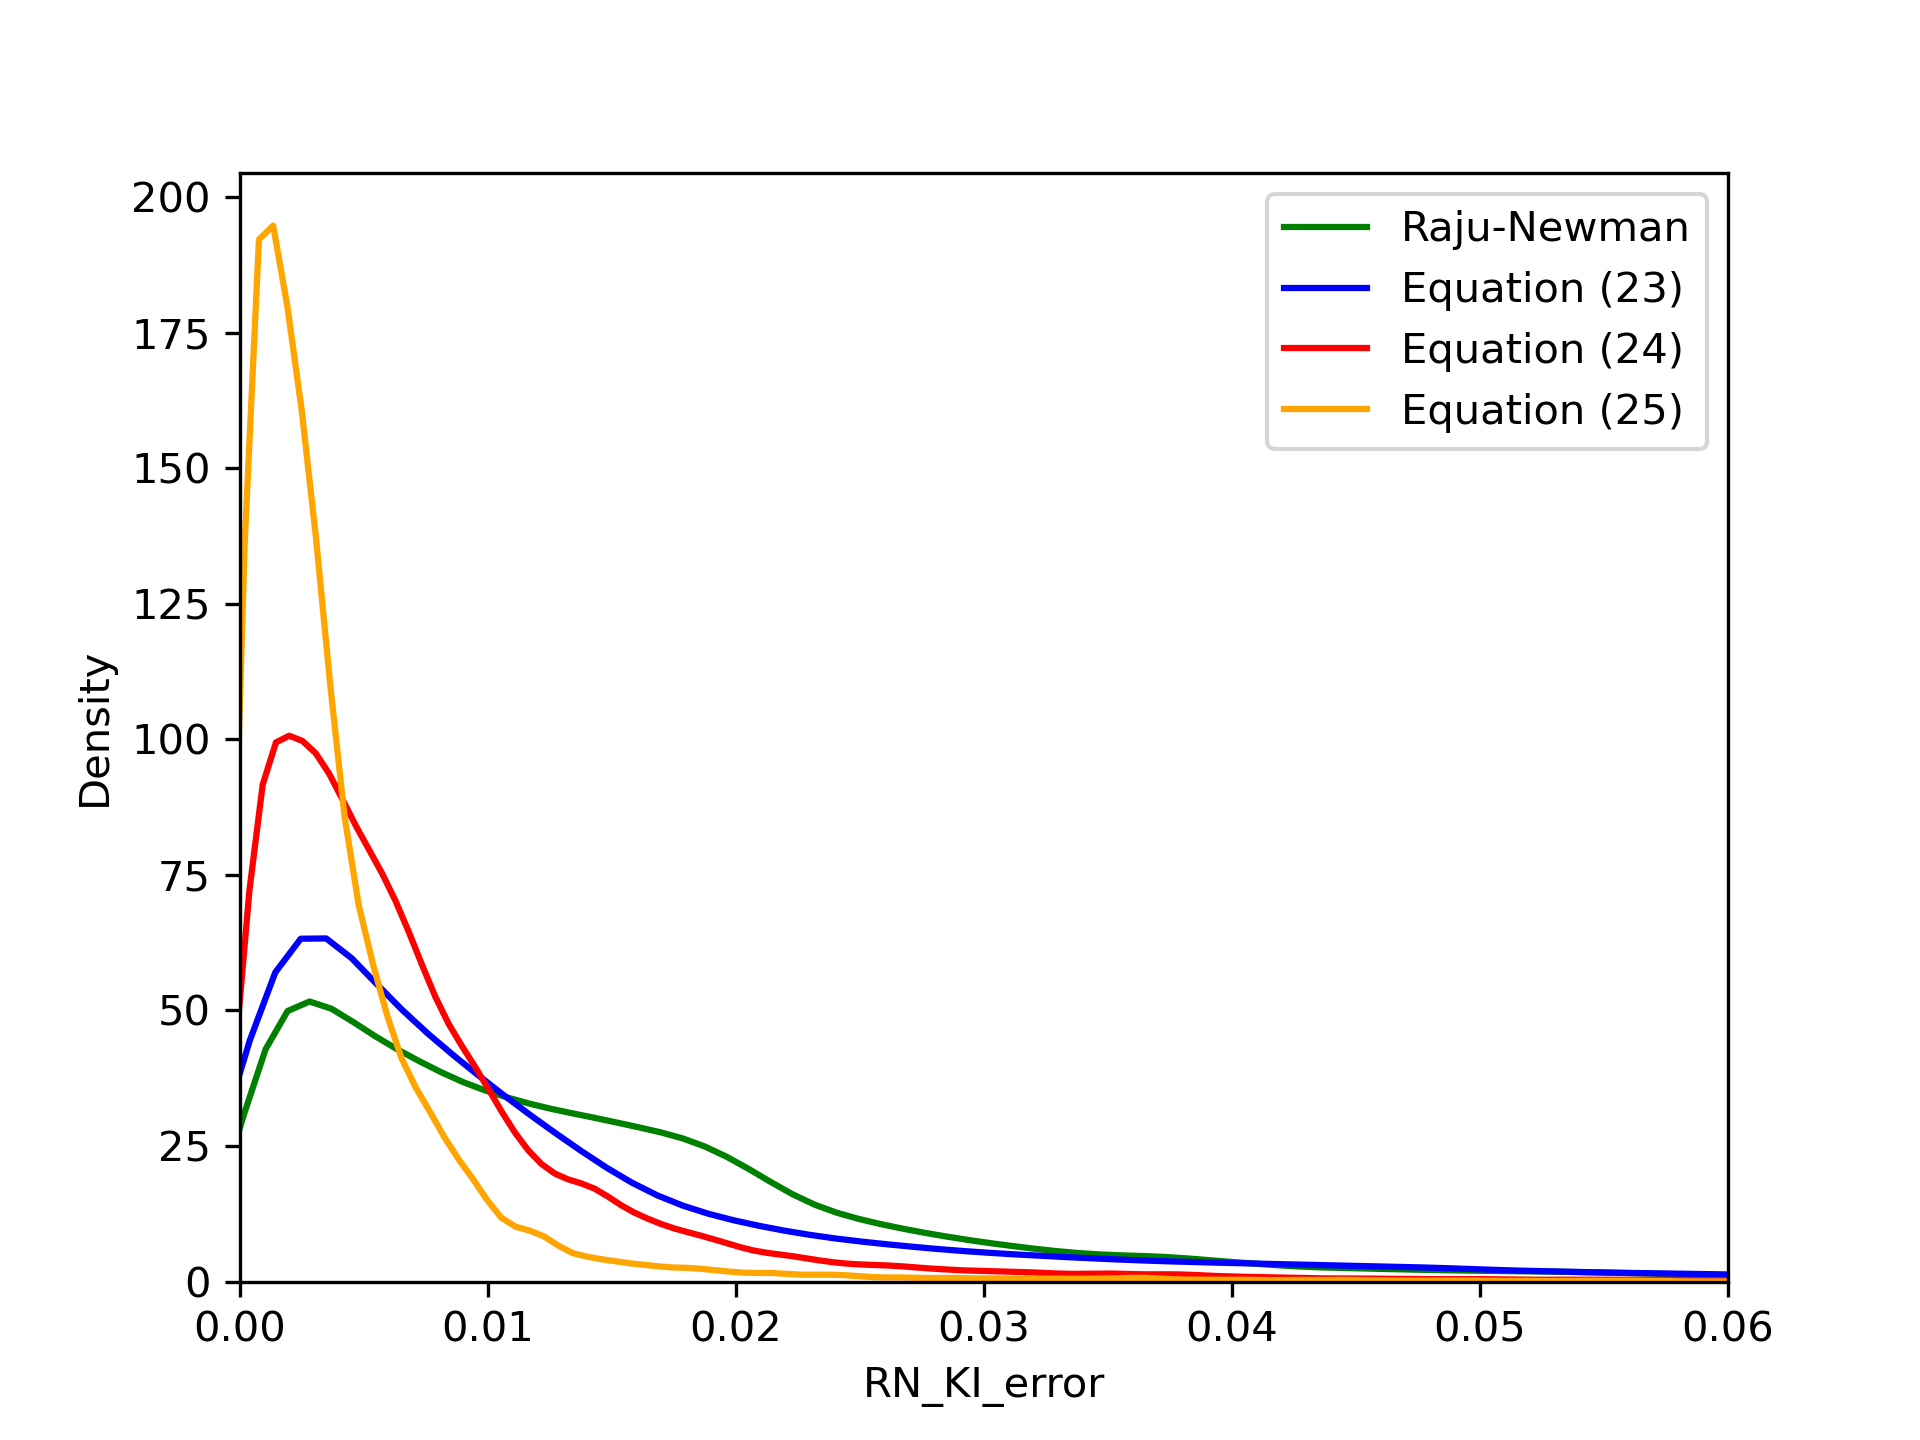
\includegraphics[width=3in]{Figures/kde_plot_everything.png} }}%
    \qquad
    \subfloat[\centering Parity plots]{{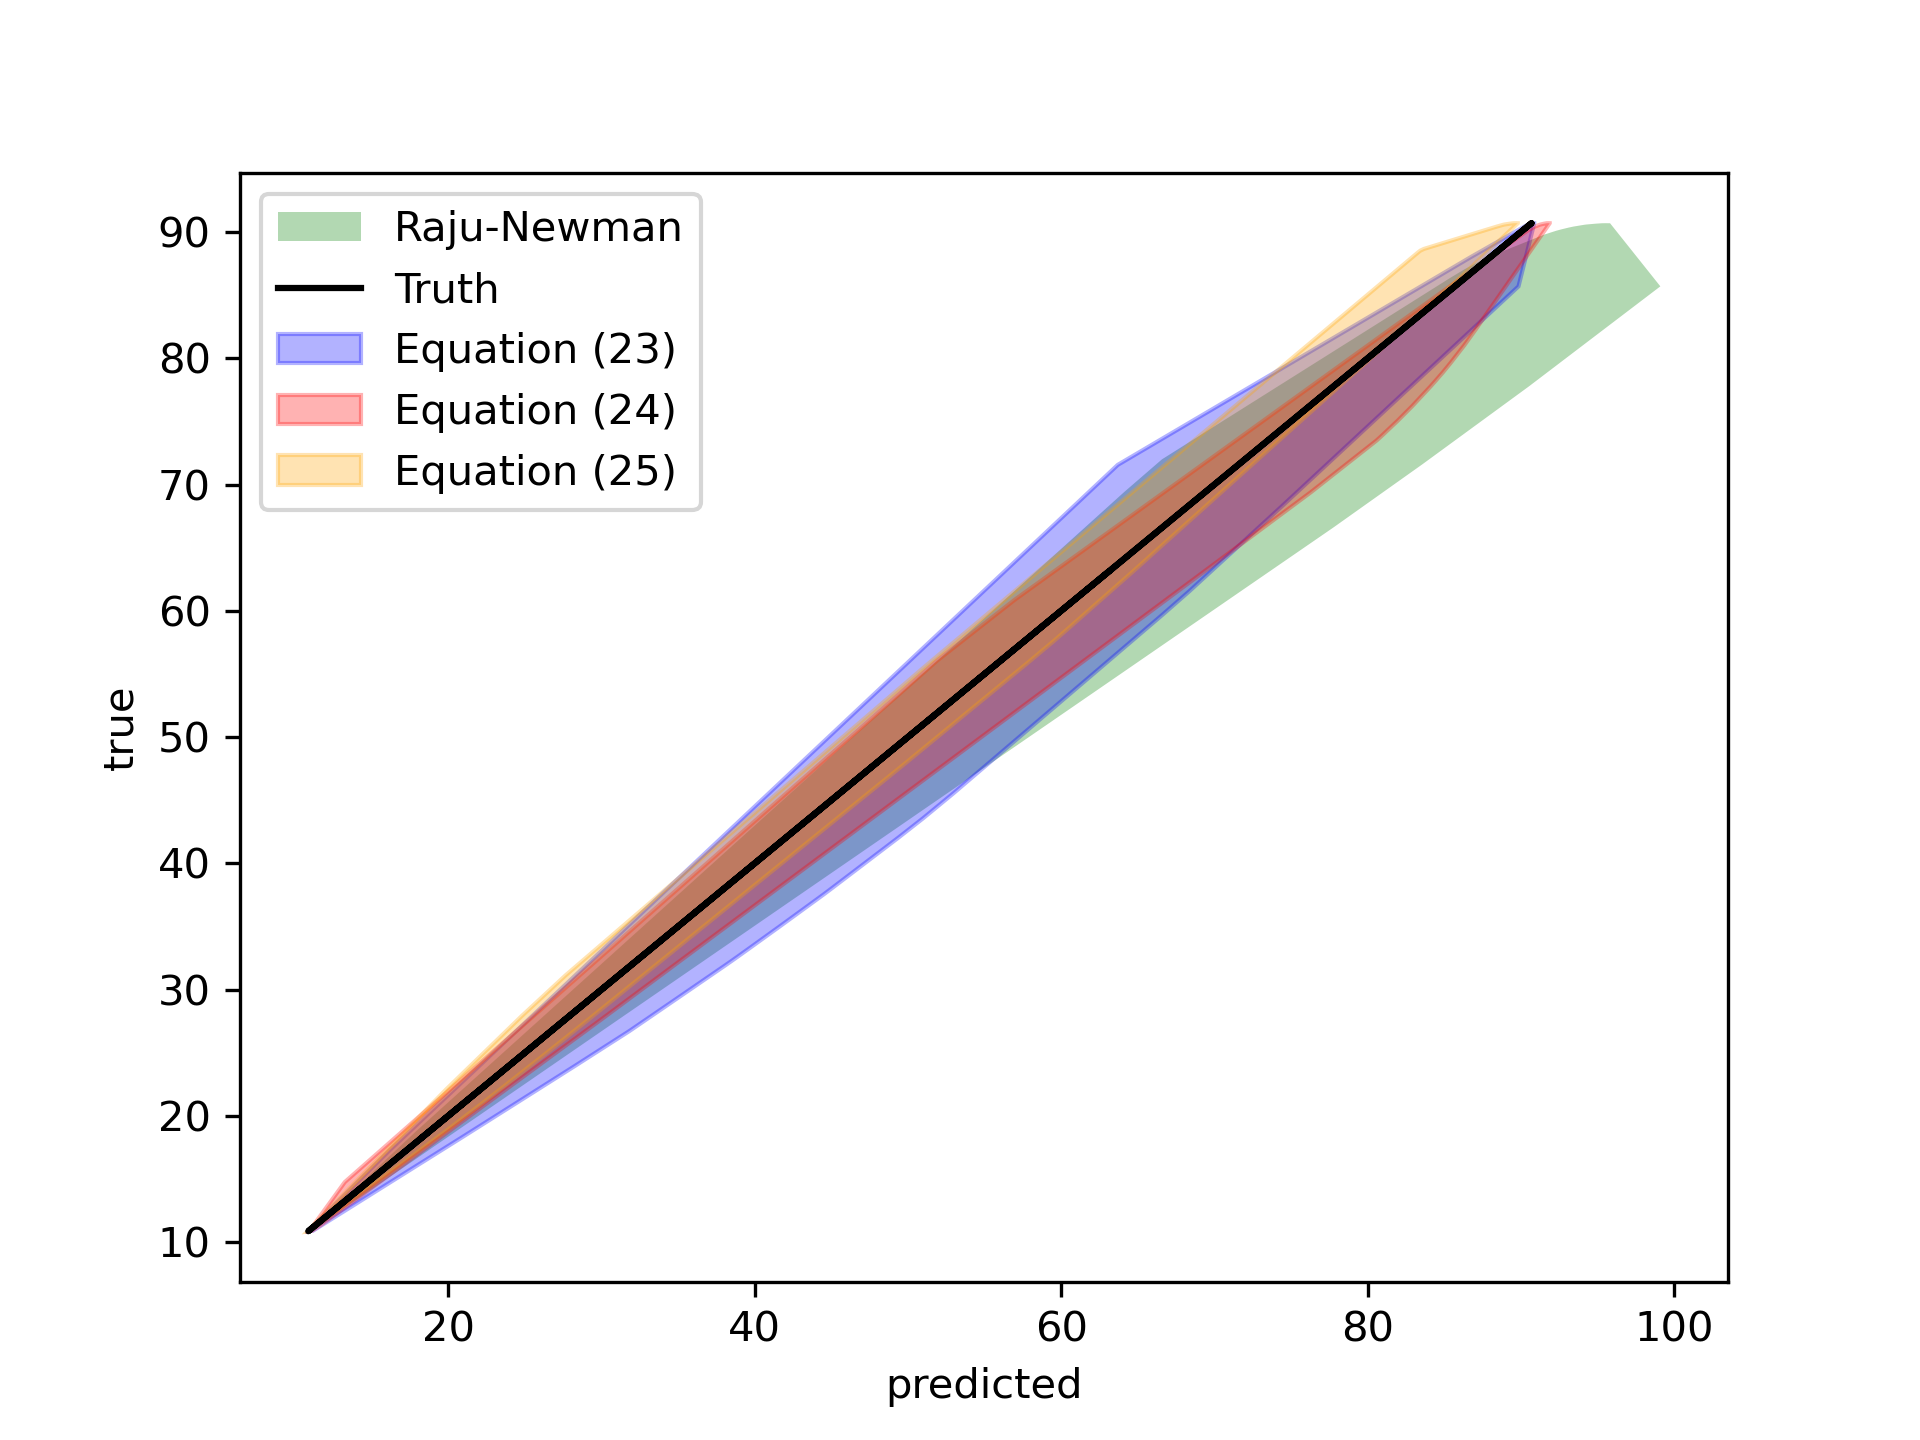
\includegraphics[width=3in]{Figures/parity_plot_everything.png} }}%
    \caption{(a) Density plot for the errors of each of the equations from the combined selection. (b) Parity plot with each of the different equations from the combined selection.}%
    \label{fig:combo_error_plots}%
\end{figure}


\begin{figure}
    \centering
    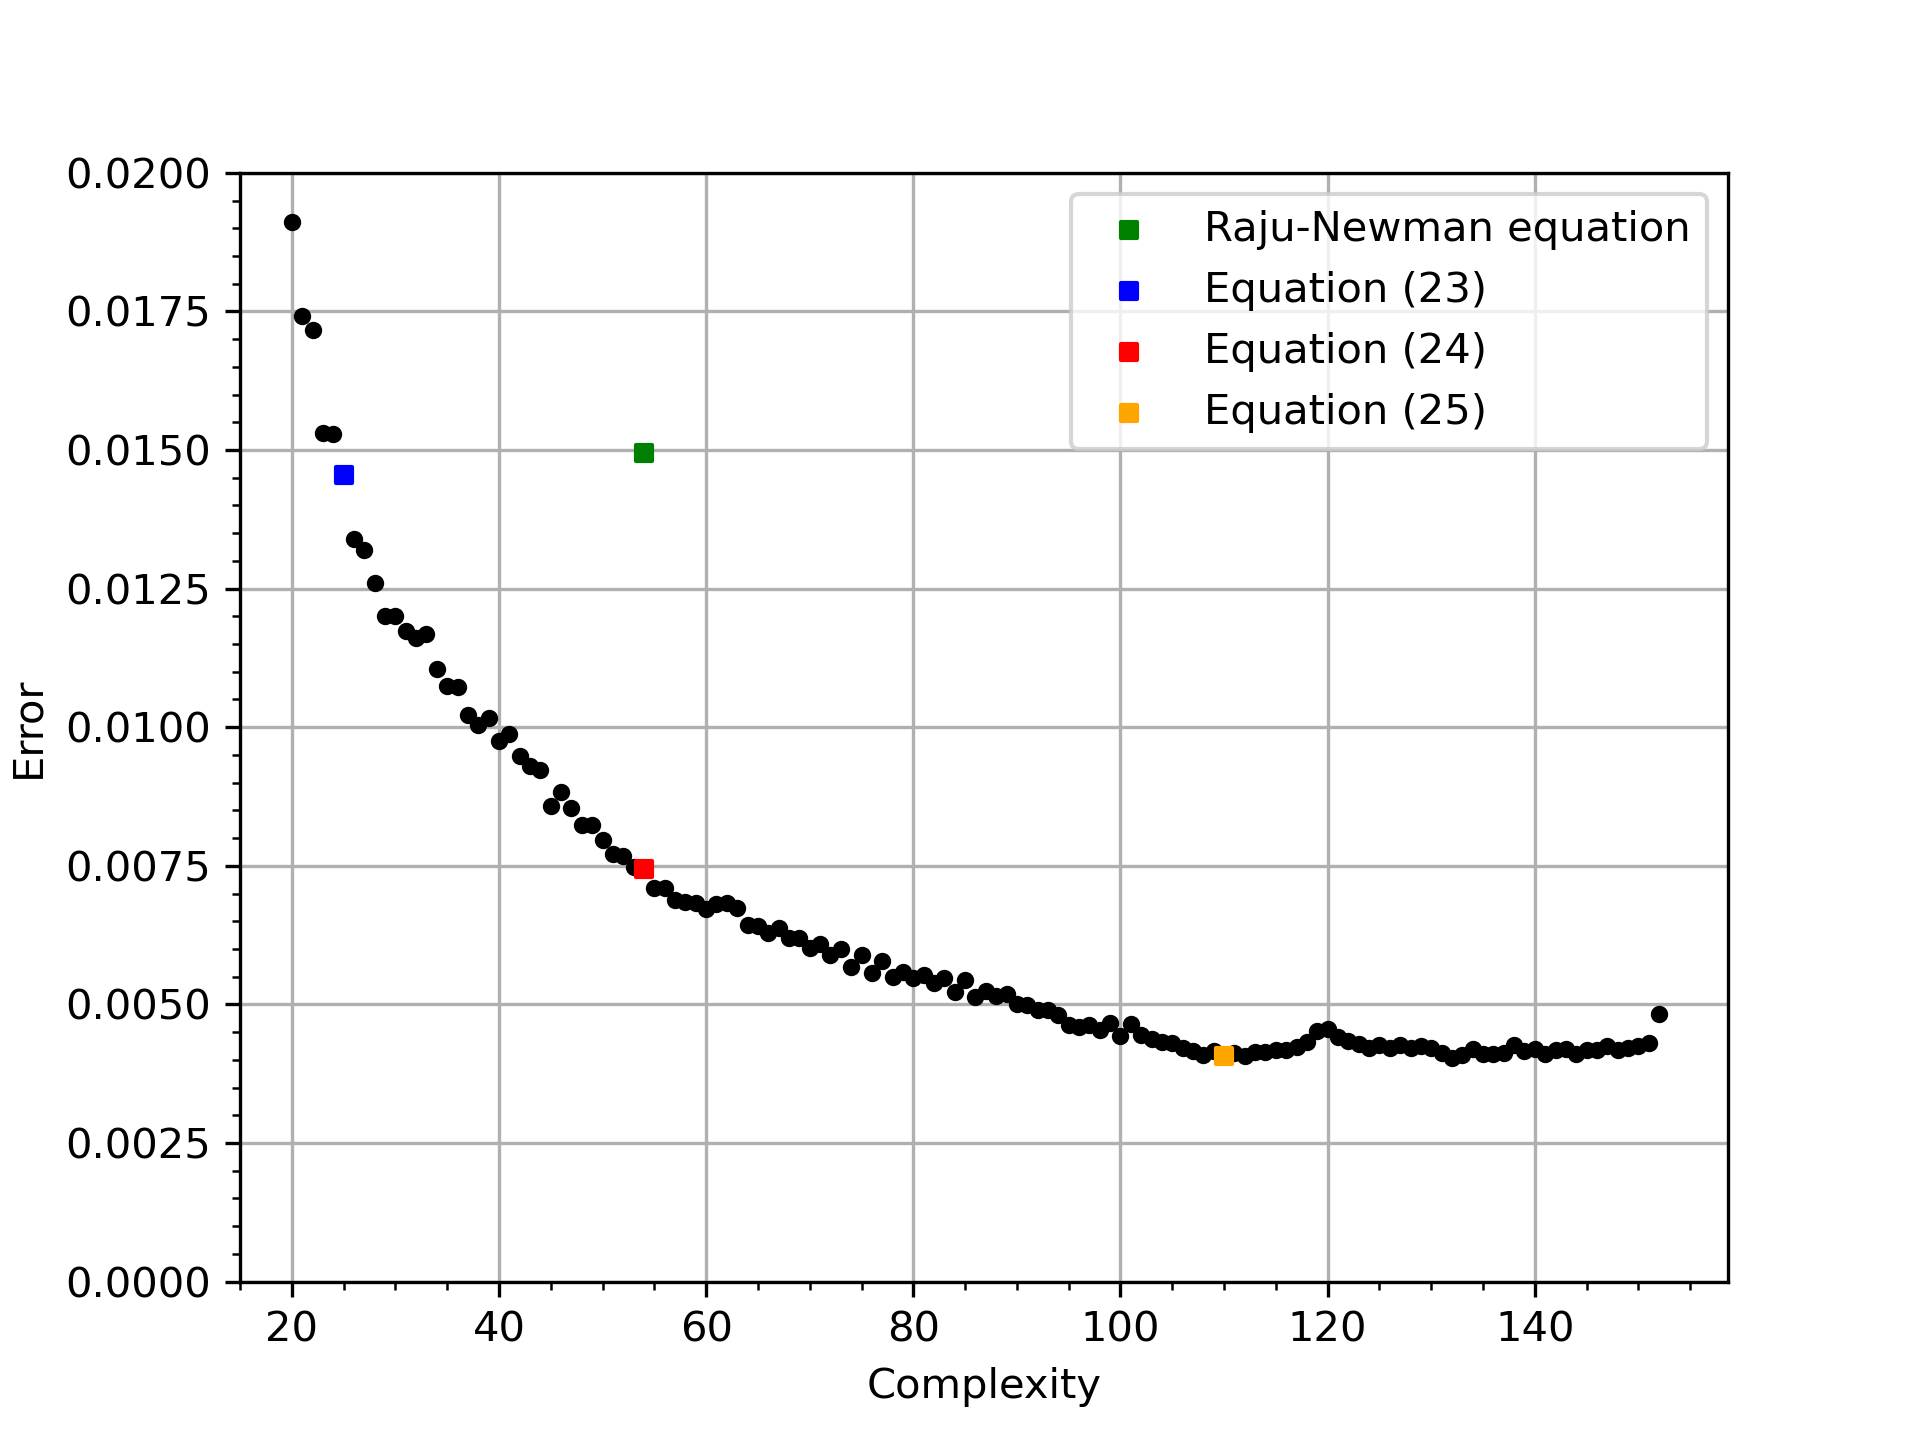
\includegraphics[width=5in]{Figures/perato_front_everything.png}
    \label{fig:perato_front_everything}
    \caption{Perato front for the models selected using all possible combinations.}
\end{figure}

\begin{figure}
    \centering
    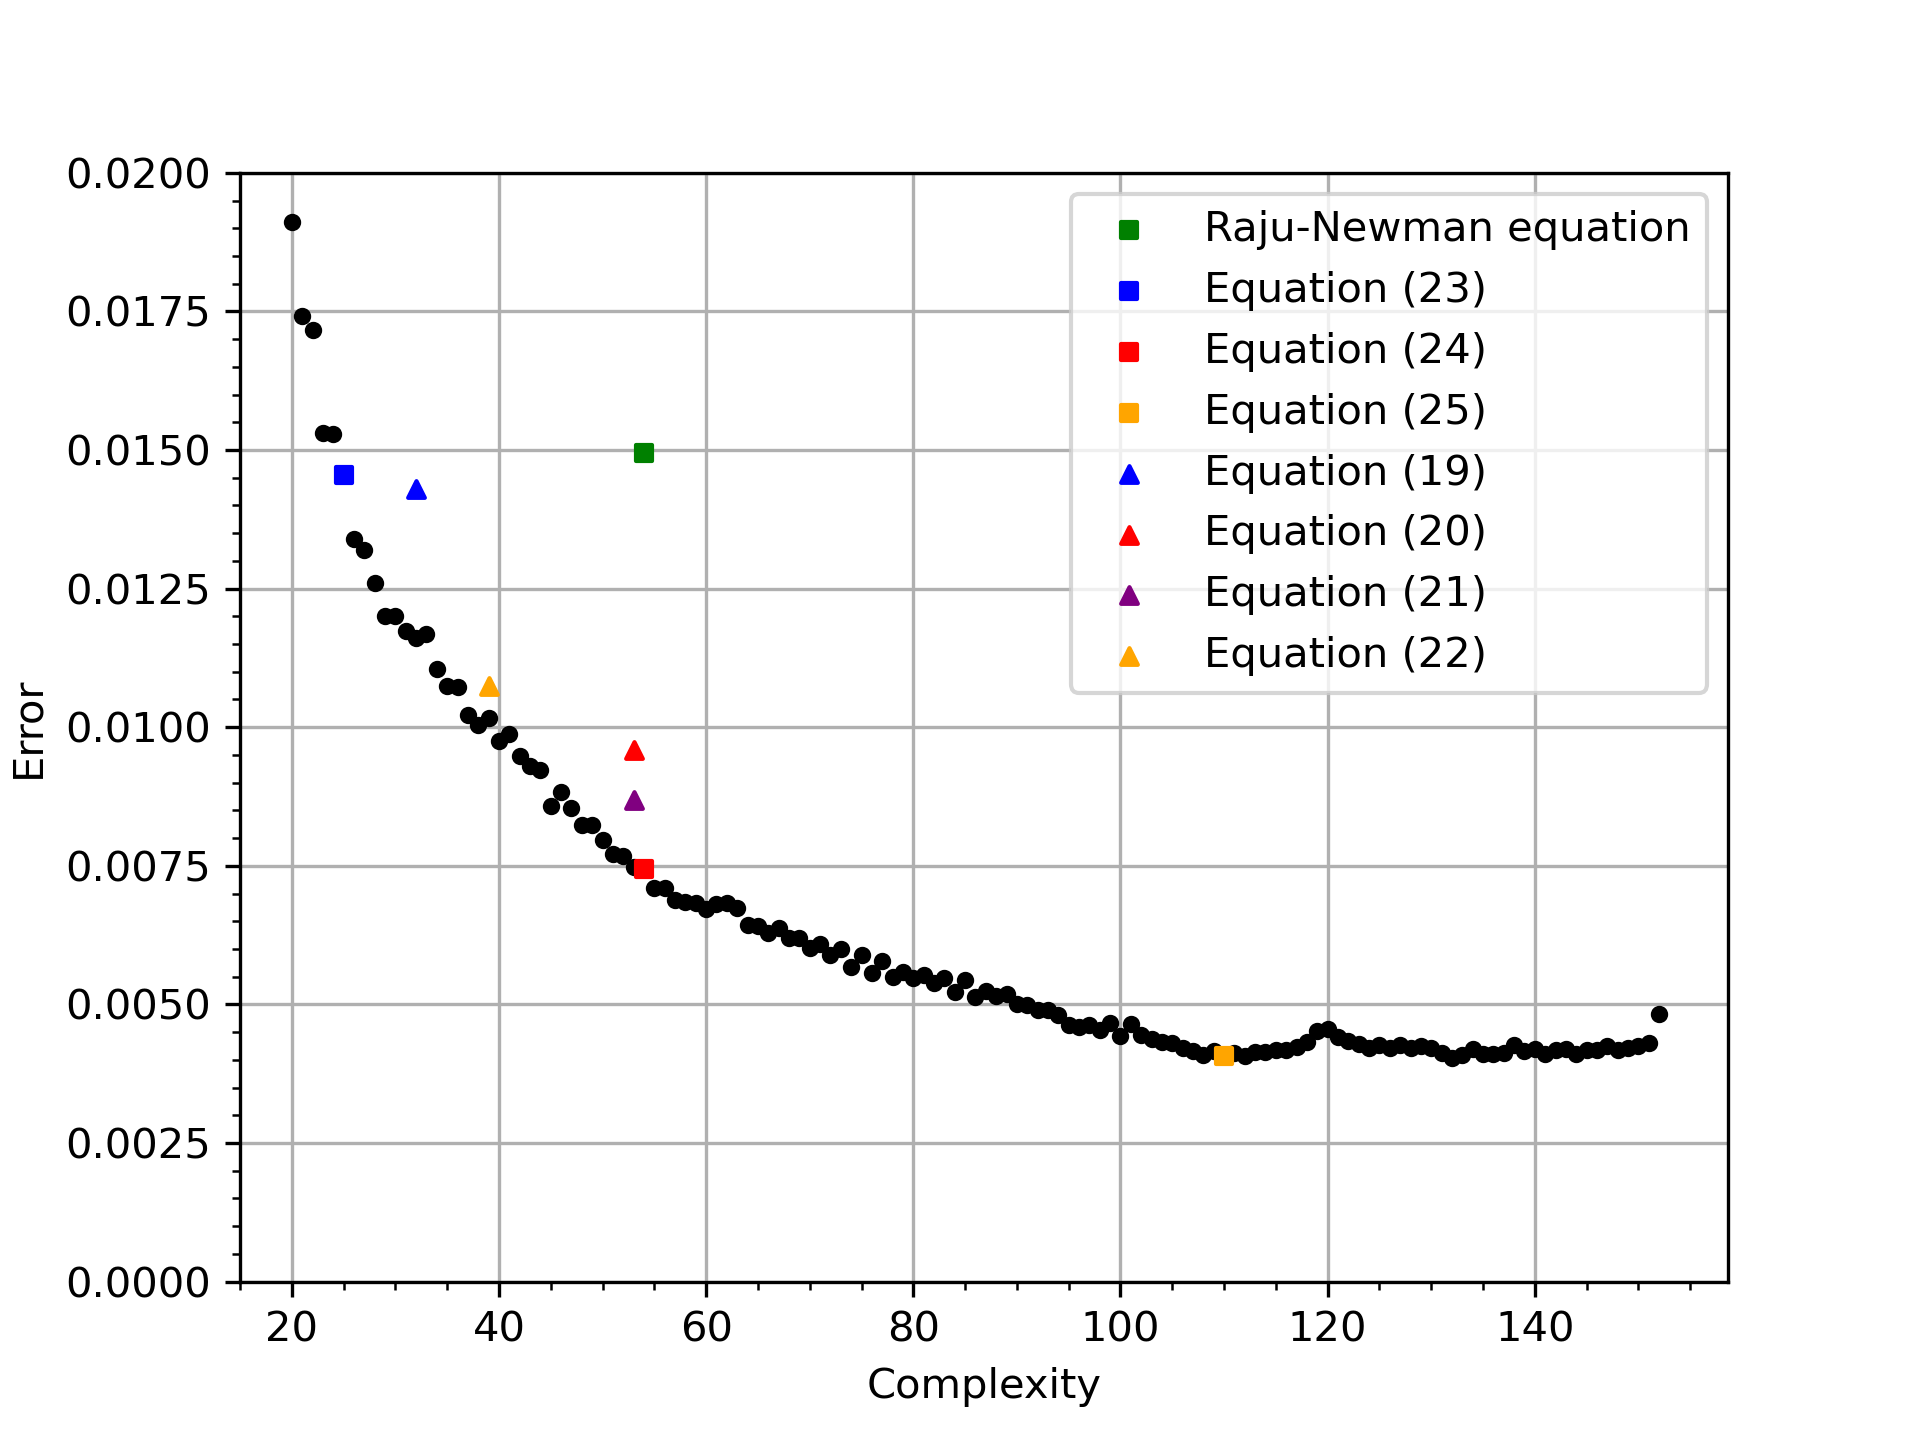
\includegraphics[width=5in]{Figures/perato_front_everything_and_more.png}
    \label{fig:perato_front_everything_ant_more}
    \caption{Perato front with all models the triangle models correspond to the models that were individually selected and the square models are the models selected using all possible combinations.}
\end{figure}





\end{document}


